%# -*- coding: utf-8-unix -*-
%%==================================================
%% thesis.tex
%%==================================================

% 双面打印
% \documentclass[doctor, fontset=adobe, openright, twoside]{sjtuthesis}
% \documentclass[bachelor, fontset=adobe, openany, oneside, submit]{sjtuthesis}
\documentclass[master, fontset=adobe, twoside, openany, submit]{sjtuthesis}
% \documentclass[%
%   bachelor|master|doctor,	% 必选项
%   fontset=adobe|windows,  	% 只测试了adobe
%   oneside|twoside,		% 单面打印,双面打印(奇偶页交换页边距,默认)
%   openany|openright, 		% 可以在奇数或者偶数页开新章|只在奇数页开新章(默认)
%   zihao=-4|5,, 		% 正文字号:小四、五号(默认)
%   review,	 		% 盲审论文,隐去作者姓名、学号、导师姓名、致谢、发表论文和参与的项目
%   submit			% 定稿提交的论文,插入签名扫描版的原创性声明、授权声明
% ]

% 逐个导入参考文献数据库
\addbibresource{bib/thesis.bib}
% \addbibresource{bib/chap2.bib}

\lstdefinestyle{myScalastyle}{
  frame=tb,
  language=scala,
  aboveskip=3mm,
  belowskip=3mm,
  showstringspaces=false,
  columns=flexible,
  basicstyle={\small\ttfamily},
  numbers=none,
  numberstyle=\tiny\color{gray},
  keywordstyle=\color{blue},
  commentstyle=\color{cyan},
  stringstyle=\color{purple},
  frame=single,
  breaklines=true,
  breakatwhitespace=true,
  tabsize=3,
}

\begin{document}

%% 无编号内容:中英文论文封面、授权页
%# -*- coding: utf-8-unix -*-
\title{分布式并行计算框架的shuffle优化}
\author{付周望}
\advisor{戚正伟教授}
% \coadvisor{某某教授}
\defenddate{2018年1月15日}
\school{上海交通大学}
\institute{软件学院}
\studentnumber{115037910032}
\major{软件工程}

\englishtitle{Efficient Shuffle Management with SCache for DAG
Computing Frameworks}
\englishauthor{\textsc{Zhouwang Fu}}
\englishadvisor{Prof. \textsc{Zhengwei Qi}}
% \englishcoadvisor{Prof. \textsc{Uom Uom}}
\englishschool{Shanghai Jiao Tong University}
\englishinstitute{\textsc{School of Software} \\
  \textsc{Shanghai Jiao Tong University} \\
  \textsc{Shanghai, P.R.China}}
\englishmajor{Software Engineering}
\englishdate{Jan, 2018}


\maketitle

\makeenglishtitle

\makeatletter
\ifsjtu@submit\relax
	
\includepdf{pdf/original.pdf}
	\cleardoublepage
	
\includepdf{pdf/authorization.pdf}
	\cleardoublepage
\else
\ifsjtu@review\relax
% exclude the original claim and authorization
\else
	\makeDeclareOriginal
	\makeDeclareAuthorization
\fi
\fi
\makeatother


\frontmatter 	% 使用罗马数字对前言编号

%% 摘要
\pagestyle{main}
%# -*- coding: utf-8-unix -*-
%%==================================================
%% abstract.tex for SJTU Master Thesis
%%==================================================

\begin{abstract}

大数据时代的到来使得分布式计算变得越来越普及。
为了快速地处理大规模的数据,有大量复杂的分布式并行计算框架被设计并使用,比如Hadoop MapReduce\cite{hadoop},Spark\cite{apachespark},Dryad\cite{dryad}, Tez\cite{tez}等。
这些分布式计算框架大多采用将用户计算逻辑用有向无环图(Directed Acyclic Graph, DAG)的方式呈现出来。
在执行DAG的每一个计算阶段时,这些计算框架大多采用了整体同步并行计算模型(Bulk-Synchronous Parallel, BSP)来对大数据进行分布式的并行批处理。

在这些相邻的计算阶段之间,shuffle,或者说跨网络的多对多分块数据的读写满足了计算逻辑对于不同数据的依赖。与此同时,shuffle的过程也带来了大量的网络数据传输。
受限于计算对于数据的依赖以及网络,磁盘等硬件性能,使得依赖于shuffle的这些任务的性能会因为shuffle的开销而受到巨大损失。
尤其是在一些需要大量shuffle数据的情境中,比如两张数据库大表的交集,shuffle的开销甚至会成为整个应用的性能瓶颈。
更重要的是,这个问题在大多数分布式并行计算框架中都普遍存在。

为了提供一种具有普遍意义的shuffle优化方案,本研究抽取了这些系统在shuffle设计中存在的一些共性问题:1)粗粒度的硬件资源管理降低了资源的可复用性, 比如使得计算资源在进行I/O操作时长时间闲置。
2)同步滞后的shuffle读取不仅增加了计算任务执行过程中对shuffle网络传输的显式等待时间,也给网络带来一个瞬时的流量高峰,进一步减慢了网络传输过程。

针对以上问题,本文提出了S(huffle)Cache --- 一个开源的即用型系统来优化DAG计算过程中的shuffle阶段。
通过在计算阶段真正执行前提取表达计算逻辑的DAG以及其中的shuffle依赖关系,SCache可以将shuffle过程从DAG计算过程中解耦合,从而提供更细粒度的硬件资源管理,提高资源利用率和复用率。
与此同时,SCache通过提前异步的shuffle传输来隐藏任务计算过程中显式的网络等待时间,同时也减缓了shuffle给网络带来的压力。
此外,SCache还利用结合应用上下文的内存管理,来实现对shuffle数据的内存缓存,进一步提升shuffle过程的效率。
为了实现以上的优化目标,本研究做出了以下主要贡献:

\begin{enumerate}
    \item 将shuffle过程从计算过程中解耦,使得shuffle过程独立到外部进行管理,从而实现了更细粒度的硬件资源管理。
    \item 结合应用的上下文对shuffle数据进行预取,既避免了同步数据读取给网络带来的压力,又能将大部分网络传输时间隐藏到计算阶段。
    \item 结合应用的上下文对shuffle数据内存管理和内存缓存,进一步提升shuffle过程的效率。
    \item 根据现有的分布式计算框架shuffle的特点设计了相应的接口(API)。通用的接口设计使得优化能被应用到不同的分布式并行计算框架当中。
\end{enumerate}

基于以上阐述,本研究课题实现了SCache,同时修改了Apache Spark对SCache进行适配。
并且通过仿真实验和Amazon AWS EC2集群上大规模数据测试来验证其优化效果。
在不同的数据集和测试程序的测试中,SCache能减少将近89\%的shuffle开销。
在TPC-DS的测试中,SCache的优化能给分布式SQL查询带来平均大约40\%的性能提升。

\keywords{\large 分布式DAG计算框架, Shuffle, 优化}
\end{abstract}

\begin{englishabstract}

Recent years have witnessed the widespread use of distributed computing in the big data area.
Numbers of sophisticated distributed data parallel computing frameworks, such as Hadoop MapReduce\cite{hadoop}, Spark\cite{apachespark}, Dryad\cite{dryad}, and Tez\cite{tez},
have been developed and deployed to accelerate the big data processing.
Most of these frameworks do the computing by transforming the application logic into Directed Acyclic Graph (DAG).
In order to increase the parallelism, each computing stage is usually managed according to the Bulk-Synchronous Parallel (BSP) model during the execution of DAG.

Shuffle, or the cross-network read and aggregation of partitioned data among tasks with data dependencies in the consecutive execution stages, 
usually brings in large network transfer. 
Due to the dependency constrains and the limited performance of disks and networks, execution of those descendant tasks could be delayed by inefficient shuffles. 
This delay can further slow down the whole application process. 
The performance degradation introduced by shuffle can become overwhelming in the shuffle intensive applications such as a join of two big tables.
Moreover, the above deficiencies of shuffle generally exist in most of the DAG data parallel computing frameworks. 
In this paper, we extract the common issues in current shuffle mechanism: 
1) The coarse granularity resource management decreases the utilization and multiplexing of hardware resources. For example, the inefficient management can keep CPU idle while tasks doing I/O operations.
2)The synchronized shuffle read increases the explicit network waiting time during task execution and brings a network burst which further slows down the shuffle read itself.

Based on the above observations, we present S(huffle)Cache --- an open source plug-in system that particularly focuses on shuffle optimization in frameworks defining jobs as DAGs. 
By extracting and analyzing the DAGs and shuffle dependencies prior to the actual task execution, 
SCache can take full advantage of the fine granularity resource management and system memory to accelerate the shuffle process. 
Meanwhile, SCache manages the shuffle data out of the frameworks and transfers data asynchronously, which helps overlap the network transfer time and avoid network burst.
In addition, SCache provides an application-context-aware in-memory shuffle data management scheme to further accelerate the shuffle process.  
In order to achieve the optimizations, we make following contributions:

\begin{enumerate}
    \item Decouple the shuffles and manage them out of the DAG data parallel computing frameworks so that the shuffle data management can become more efficient.
    \item Implement the shuffle data pre-fetch with application context so that the network burst can be avoided and the network transfer time can be overlapped in execution phases.
    \item Implement the application-context-aware in-memory shuffle data management to accelerate the shuffle process.
    \item Design and implement the general APIs for the DAG data parallel computing frameworks so that the optimizations can be applied easily.
\end{enumerate}

We have implemented SCache and customized Spark to use it as the external shuffle service and co-scheduler. 
The performance of SCache is evaluated with both simulations and testbed experiments on a 50-node Amazon EC2 cluster.
Those evaluations have demonstrated that, by incorporating SCache, the shuffle overhead of Spark can be reduced by nearly 89\%, 
and the overall completion time of TPC-DS queries improves 40\% on average.


\englishkeywords{\large Distributed DAG frameworks, Shuffle, Optimization}
\end{englishabstract}



%% 目录、插图目录、表格目录
\tableofcontents
\listoffigures
\addcontentsline{toc}{chapter}{\listfigurename} %将插图目录加入全文目录
\listoftables
\addcontentsline{toc}{chapter}{\listtablename}  %将表格目录加入全文目录
\listofalgorithms
\addcontentsline{toc}{chapter}{算法索引}        %将算法目录加入全文目录

% %# -*- coding: utf-8-unix -*-
\chapter{主要符号对照表}
\label{chap:symb}

\begin{longtable}{rl}
$\epsilon$     & 介电常数 \\
 $\mu$ 		& 磁导率 \\
 $\epsilon$     & 介电常数 \\
 $\mu$ 		& 磁导率 \\
 $\epsilon$     & 介电常数 \\
 $\mu$ 		& 磁导率 \\
 $\epsilon$ 	& 介电常数 \\
 $\mu$ 		& 磁导率 \\
 $\epsilon$     & 介电常数 \\
 $\mu$ 		& 磁导率 \\
 $\epsilon$     & 介电常数 \\
 $\mu$ 		& 磁导率 \\
 $\epsilon$     & 介电常数 \\
 $\mu$ 		& 磁导率 \\
 $\epsilon$ 	& 介电常数 \\
 $\mu$ 		& 磁导率 \\
 $\epsilon$     & 介电常数 \\
 $\mu$ 		& 磁导率 \\
 $\epsilon$     & 介电常数 \\
 $\mu$ 		& 磁导率 \\
 $\epsilon$     & 介电常数 \\
 $\mu$ 		& 磁导率 \\
 $\epsilon$ 	& 介电常数 \\
 $\mu$ 		& 磁导率 \\
 $\epsilon$     & 介电常数 \\
 $\mu$ 		& 磁导率 \\
 $\epsilon$     & 介电常数 \\
 $\mu$ 		& 磁导率 \\
 $\epsilon$     & 介电常数 \\
 $\mu$ 		& 磁导率 \\
 $\epsilon$ 	& 介电常数 \\
 $\mu$ 		& 磁导率 \\
 $\epsilon$     & 介电常数 \\
 $\mu$ 		& 磁导率 \\
 $\epsilon$     & 介电常数 \\
 $\mu$ 		& 磁导率 \\
 $\epsilon$     & 介电常数 \\
 $\mu$ 		& 磁导率 \\
 $\epsilon$ 	& 介电常数 \\
 $\mu$ 		& 磁导率 \\
 $\epsilon$     & 介电常数 \\
 $\mu$ 		& 磁导率 \\
 $\epsilon$     & 介电常数 \\
 $\mu$ 		& 磁导率 \\
 $\epsilon$     & 介电常数 \\
 $\mu$ 		& 磁导率 \\
 $\epsilon$ 	& 介电常数 \\
 $\mu$ 		& 磁导率 \\
 $\epsilon$     & 介电常数 \\
 $\mu$ 		& 磁导率 \\
 $\epsilon$     & 介电常数 \\
 $\mu$ 		& 磁导率 \\
 $\epsilon$     & 介电常数 \\
 $\mu$ 		& 磁导率 \\
\end{longtable}
 % 主要符号、缩略词对照表

\mainmatter	% 使用阿拉伯数字对正文编号

%% 正文内容
\pagestyle{main}
\section{Introduction}
\ifrevision
\reversemarginpar
\marginnote{60D}
\fi
Recent years have witnessed widespread use of sophisticated frameworks, such as Hadoop MapReduce \cite{hadoop}, Dryad \cite{dryad}, Spark \cite{spark}, and Apache Tez \cite{tez}.
\hlyellow{
Most of them define jobs as directed acyclic graphs (DAGs), such as map-reduce pipeline in Hadoop MapReduce, lineage of resilient distributed datasets (RDD) in Spark, vertices and edges in Dryad and Tez, etc.
}
Despite the differences among data-intensive frameworks, their communication is always structured as a shuffle phase,  which takes place between successive computation stages. 
Such shuffle phase places significant burden for both the disk and network I/O, thus heavily affecting the end-to-end application performance. 
For instance, a MapReduce trace analysis from Facebook shows that shuffle accounts for 33\% of the job completion time on average, and up to 70\% in shuffle-heavy jobs \cite{managing}.

Although continued efforts of performance optimization have been made among a variety of computing frameworks \cite{sync, babu, tachyon, pacman, quincy, delay}, 
the shuffle is often poorly optimized in practice.
% take over shuffle
%shuffle characteristic
In particular, we observe that one major deficiency lies in a lack of fine-grained, coordinated management among different system resources.
%In the current practice, the shuffle phase is often split into two parts --- \textit{shuffle read} and \textit{shuffle write}. 
As Figure \ref{fig:workflow} shows, the \textit{shuffle write} is responsible for writing intermediate results to disk, which is attached to the tasks in ancestor stage (i.e., map task).  
And the \textit{shuffle read} fetches intermediate results from remote disks through network, which is commonly integrated as part of the tasks in descendant stage (i.e., reduce task). 
Once scheduled, a fixed bundle of resources (i.e., CPU, memory, disk and network) named \textit{slot} is assigned to each of the computation task, and the resources are released only after the task finishes.
Such task aggregation together with the coarse-grained scheduling effectively simplifies task management.
\hlyellow{
However, since a cluster has a limited number of slots, attaching the I/O intensive shuffle phase to the CPU/memory intensive computation phase results in a poor multiplexing between computational and I/O resources.
}
%The map task in Figure \ref{fig:workflow} well explains such deficiency: the I/O resource allocated to the stage is always idle during the computation time, and the computation/memory resource is totally wasted during the shuffle write attached to it, and vice versa.
\begin{figure}
	\centering
	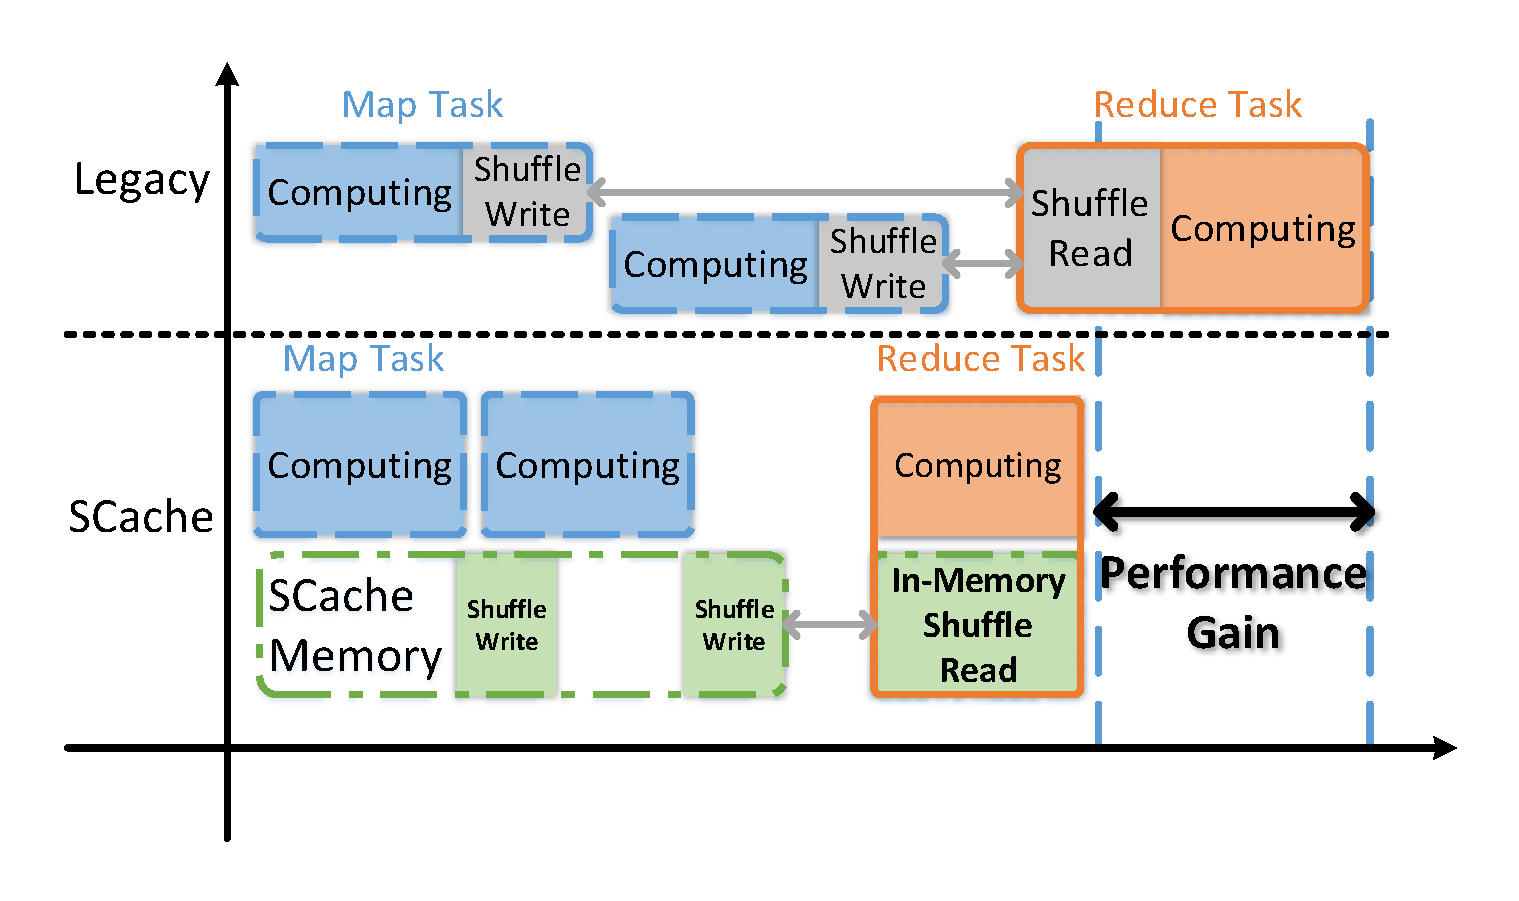
\includegraphics[width=\linewidth]{fig/workflow}
	\caption{Workflow Comparison between Legacy DAG Computing Frameworks and Frameworks with SCache}
	\label{fig:workflow}
	\vspace{-1em}
\end{figure}

Moreover, the shuffle read phase introduces all-to-all communication pattern across the network, and such network I/O procedure is also poorly coordinated.
Note that the shuffle read phase starts fetching data only after the corresponding reduce tasks start.
Meanwhile, the reduce tasks belonging to a same execution phase are scheduled at the same time by default. 
As a result, all the corresponding reduce tasks start fetching shuffle data almost simultaneously.
Such synchronized network communication causes a burst demand for network I/O, which in turn greatly enlarges the shuffle read completion time. 
To desynchronize the network communication, an intuitive way is to launch some tasks in the descendent stage earlier, such as "slow-start" from Hadoop MapReduce\cite{hadoop}. 
However, such early-start is by no means a panacea. 
\hlyellow{
This is because the early-start always introduces an extra early allocation of slot, which slows down the current stage execution.
}
% This is because although the reduce tasks can start fetching data earlier, the computation can only take place after all the data is ready. 

%In one word, existing solutions suffer from either inefficient use of network I/O, or a waste of computational resources (i.e., CPU and memory) caused by task pre-launching.

%For example, Apache Hadoop \cite{hadoop} provides an \emph{early start} mechanism that launches reduce tasks after a certain portion (5\% by default) of map tasks has completed, which is adopted in many of the recent works \cite{ihadoop, ishuffle, dynmr}.
% DAG computing framworks deriving from MapReduce \cite{mapreduce} contains a hard barrier between computing stages. The terminology of this barrier is \textit{shuffle}. Shuffle contains two parts on the connecting stages -- \textit{shuffle write} and \textit{shuffle read}. On the side of ancestor stages, \textit{shuffle write} is resoponsible for writing intermediate results to disk. On the side of descendant stage, \textit{shuffle read} fetches intermediate results from remote disks through network. Although highly optimized in other factors, the shuffle of framework is still primitive.  The coarse design of shuffle introduce a significiant performance overhead.
% % design inconsistent
% For instance, a MapReduce trace analysis from Facebook shows that shuffle accounts for 33\% JCT on average, up to 70\% in shuffle-heavy jobs \cite{managing}.
% shuffle operations
% three resource coordinate 不好
% 计算和I/O couple, why
% why disk, reason!!!, 不重视
% common problems

To make things worse, we note that the above deficiencies generally exist in most of the DAG computing frameworks. 
As a result, even we can effectively resolve the above deficiencies by modifying one framework, updating one application at a time is impractical given the sheer number of computing frameworks available today.

% The main defect of current shuffle design is coarse granularity of resource allocation during the task scheduling.
% Nearly all task scheduling algorithms in DAG frameworks use time slotted model. Specifically, when a task is launched, the framework offers it a bundle of resources (i.e. CPU and memory), which are dedicated to this task during the time in its "slot".
% But for a task, the resources demand changes during different phases. The computing phase is CPU and memory intensive. The shuffle, instead, is I/O intensive.
% As shown in the upper part of Figure \ref{fig:workflow}, this "slot" can be released until the map tasks finish \textit{shuffle write} on disk. And the "slot" is occupied when the reduce tasks begin to read shuffle data from remote nodes through network, which is presented as \textit{shuffle read}. This inconsistency between demands and allocation results in a severe resource underutilization, which slow down the framework.

% Another drawback of current shuffle is the synchronized shuffle read. When all the reduce tasks are scheduled, the shuffle fetch of each task starts almost simultaneously, which may cause congestion of network and delay the shuffle read. The straight forward way to avoid network burst is to start reduce tasks earlier. Apache Hadoop \cite{hadoop} provides a mechanism that schedules reduce tasks when a certain portion of map tasks completed. So that the shuffle delay can be mitigated. Other publications also purpose solutions to pre-schedule reduce tasks \cite{ihadoop, ishuffle, dynmr}. However this early scheduling of reduce tasks occupies new task slots, which degrades system performance. To this end, we proposed a question for this cross-frameworks issue, \textit{can we efficiently optimize shuffle without manually change every DAG framework?}




% 针对性的提出这三个点
% three resource coordinate 不好
% 计算和I/O couple, why
% why disk, reason, 不重视
% common problems
% 总起:普适性工具
% pre-fetch but not pre-execute
% byproduct: more balance
% memory instead of disk

% challenge point by point, inside the problem

Can we efficiently optimize the data shuffling without significantly changing every framework?
In this paper, we answer this question in the affirmative with S(huffle)Cache, an open source plug-in system which provides a shuffle-specific optimization for different DAG computing frameworks.
Specifically, SCache takes over the whole shuffle phase from the underlying framework by providing a cross-framework API for both shuffle write and read.
SCache's effectiveness lies in the following two key ideas.
First, SCache decouples the shuffle write and read from both map and reduce tasks.
Such decoupling effectively enables fine-grained resource management and better multiplexing between the computational and I/O resources.
\hlyellow{
In addition, SCache pre-schedules the reduce tasks \emph{without launching} them and pre-fetches the shuffle data for the reduce tasks.
Such pre-scheduling and pre-fetching effectively overlap the network transfer time, desynchronize the network operations, 
and avoid the extra early allocation of slots.
}
%In this paper, we introduce S(huffle)Cache, an plugin system to remove shuffle latency for DAG frameworks. SCache takes over the management of shuffle and I/O resources to acheive a fine granularity scheduling of tasks. In addition, SCache pre-schedules the reduce tasks without launching them and perform shuffle data pre-fetch to break the synchronization of shuffle fetch. In order to provide a general optimization for different DAG frameworks, SCache decouple the shuffle process from computing and  provide a cross-frameworks API for shuffle write and read.

The workflow of DAG framework with SCache is presented in Figure \ref{fig:workflow}. 
\hlyellow{
SCache hijacks the shuffle data of a map task in memory space. 
The disk operation is skipped and the slot is released after memory copy. 
The in-memory shuffle data is immediately pre-fetched through network after pre-scheduling of reduce tasks. 
The application-context-aware memory management caches the shuffle data in memory before the start of the reduce task.
By applying these optimizations, SCache can help the DAG framework achieve a significant performance gain. 
}

The main challenge to achieve this optimization is \textit{pre-scheduling reduce tasks without launching}. 
% It is not critical for the simple DAG computing such as Hadoop MapReduce \cite{mapreduce}. 
\hlyellow{
Firstly, the complexity of DAG can amplify the defects of na\"{i}ve scheduling schemes. 
In particular, randomly assigning reduce tasks might result in a collision of two heavy tasks on one node. 
This collision can aggravate data skew, thus hurting the performance. 
Secondly, pre-scheduling without launching violates the design of most frameworks that launch a task after scheduling.
To address the challenges, we propose a heuristic task pre-scheduling scheme with shuffle data prediction and a task co-scheduler} (Section \ref{opt}).

Another challenge is the \textit{in-memory data management}. 
To prevent shuffle data touching the disk, SCache leverages extra memory to store the shuffle data. 
However, the memory is a precious resource for DAG computing. 
To minimize the reserved memory while maximizing the performance gain, we propose two constraints: all-or-nothing and context-aware (Section \ref{memorymanage}).
%The memory management scheme follows these two contraints to switch shuffle data blocks on and off reserved memory.

We have implemented SCache and a customized Apache Spark \cite{apachespark}. 
The performance of SCache is evaluated with both simulations and testbed experiments on a 50-node Amazon EC2 cluster. 
We conduct basic test GroupByTest. 
We also evaluate Terasort \cite{spark-tera} benchmark and standard workloads like TPC-DS \cite{tpcds} for multi-tenant modeling. 
In a nutshell, SCache can eliminate explicit shuffle process by at most $89\%$ in varied application scenarios. 
More impressively, SCache reduces $~40\%$ of overall completion time of TPC-DS queries on average.


%# -*- coding: utf-8-unix -*-
%%==================================================
%% chapter02.tex for SJTU Master Thesis
%%==================================================

\chapter{Shuffle特性分析}
\label{chap:observations}

本章首先分析了shuffle在目前分布式DAG计算框架中的特性,然后通过对其特征的研究,结合分布式DAG计算框架的特性,探索其优化的方向。

\section{Shuffle特性}
在分布式DAG计算框架中,shuffle被用来实现一个在计算过程中任务的多对多的部分数据依赖。
同时也代表了一次计算集群内部节点多对多的网络数据传输。
为了便于理解,本文用map阶段来代表产生shuffle数据的DAG计算阶段,用reduce阶段代表获取shuffle数据作为输入的计算阶段。

在图\ref{fig:workflow}中,我们呈现了一个shuffle在现有分布式DAG框架中局部的工作流程, 该流程由两个map任务和一个reduce任务组成。
如图\ref{fig:workflow}所示,其中的“shuffle write”表示一个map任务将计算产生的中间结果写入到本地磁盘的过程。
这个过程会在map任务完成对所有输入数据的计算之后开始。
在每一个map任务内部,计算框架会根据用户定义的计算方法和现阶段的数据,对于其中一个数据分区(partition)进行计算。
计算完成之后,map任务就会根据用户定义的分区函数(比如哈希分区或者排序分区),将计算产生的中间结果(键值对)进行分块存储。
其中存储这些代表中间结果的键值对的数据块的数目等同于下一个计算阶段(reduce)的任务数目。
这些分块的数据即在shuffle阶段通过网络传输的数据。这些数据块往往会在分块结束之后被写入本地磁盘。

在reduce阶段开始真正的计算之前,首先要通过网络从远程的节点的磁盘上拉取map阶段产生的属于该任务输入的部分shuffle数据块,即图\ref{fig:workflow}中的“shuffle read”部分。

可以看到在传统的分布式DAG计算框架中,受限于粗粒度的资源调度机制,无论是“shuffle write”还是“shuffle read”,这些I/O密集型操作都是由计算任务(task)来执行的。
而计算任务在分布式DAG计算框架的调度中,是按照集群中计算资源的负载进行均衡调度的。
也就是说在分配计算任务时,分布式DAG计算框架的调度器默认其为计算密集型任务,因此会根据各个节点计算资源(比如CPU的空闲核数)来申请资源并调度任务。
但是任务被调度之后,却没有充分利用计算资源,反而在占用计算资源的情况下进行大量的I/O操作。
正因为这种粗粒度的调度和集成在计算任务中的I/O操作,使得硬件资源的利用率和复用率严重受损,进而损害了计算框架本身的性能。
有相关研究表明,Yahoo!公司中60\%的MapReduce工作和Facebook公司中20\%的MapReduce工作中存在大量的shuffle数据\cite{shufflewatcher}。
对于这些存在大量shuffle的工作中,shuffle传输所带来的延迟甚至会成为整个工作完成时间的瓶颈。
比如在一份Facebook公司公开的MapReduce任务日志中,shuffle过程的平均占用了整个工作完成时间的33\%。
对于那些存在大量shuffle的工作,shuffle的开销甚至最多占用了整个工作完成时间的70\%\cite{managing}。

\begin{figure}[!htp]
	\centering
	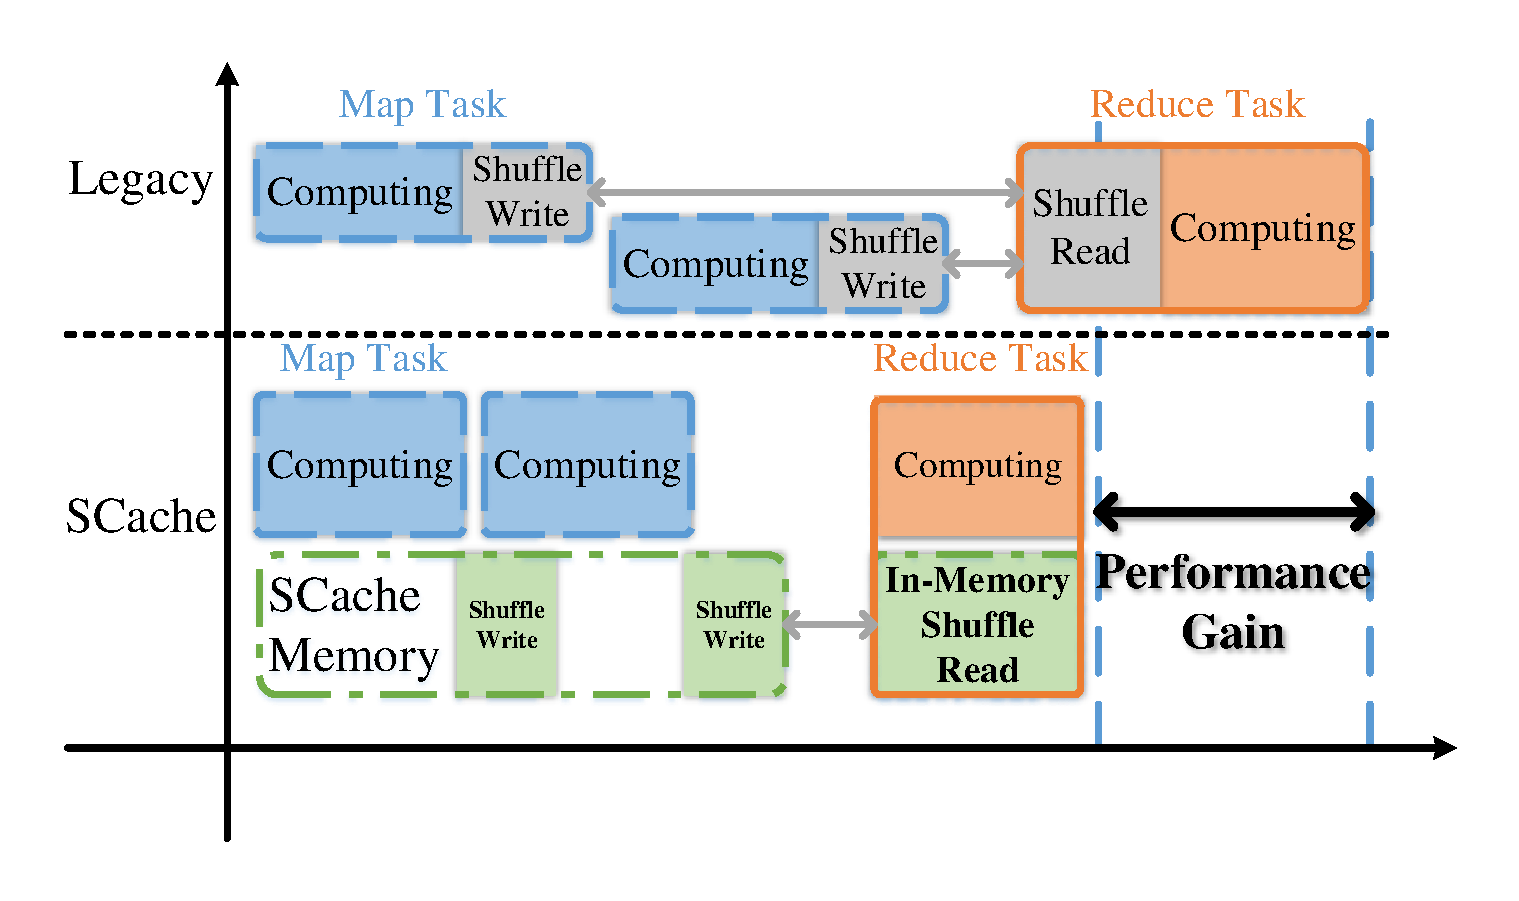
\includegraphics[width=\textwidth]{../../PPoPP-2018/fig/workflow.pdf}
	\bicaption[fig:workflow]{传统分布式DAG计算框架工作流程与在SCache协同下工作流程的比较}{传统分布式DAG计算框架工作流程与在SCache协同下工作流程的比较}{Fig}{Workflow Comparison between Legacy DAG Computing
	Frameworks and Frameworks with SCache}
\end{figure}

\section{基于shuffle特性的分析}

为了满足计算逻辑中的部分依赖,shuffle这个过程在分布式DAG的计算过程中是无法避免的。
但是我们能否通过改进shuffle的过程来减少其对计算框架性能的影响呢?
为了探索对其优化的可能性,我们在一个由5个Amazon AWS EC2 m4.xlarge\cite{aws}节点组成的集群中运行了一些具有代表性的Spark应用。
在运行这些应用的同时,我们测量了每个节点的CPU利用率,磁盘和网络的吞吐率,并且收集了每个应用的执行信息。
在图\ref{fig:util}中,我们展示了在运行一个Spark GroupByTest应用时一个节点上的硬件资源利用率随时间变化的结果。
Spark GroupByTest是一个包含两轮计算阶段,中间通过一次shuffle连接的简单应用。
图中的“execution”部分表示了从第一个计算任务启动到最后一个计算任务结束的时间,
“shuffle write”阶段表示从第一个任务shuffle数据块被写入开始到最后一个任务的最后一个数据块写入结束的时间,
“shuffle read and execution”则表示从第一个reduce任务开始获取shuffle数据并执行到所有reduce任务执行结束的时间。

从单节点的硬件资源率用率和任务执行的时间分布,结合剩余节点采集的数据,我们发现以下一些问题。

\begin{figure}[!htp]
	\centering
	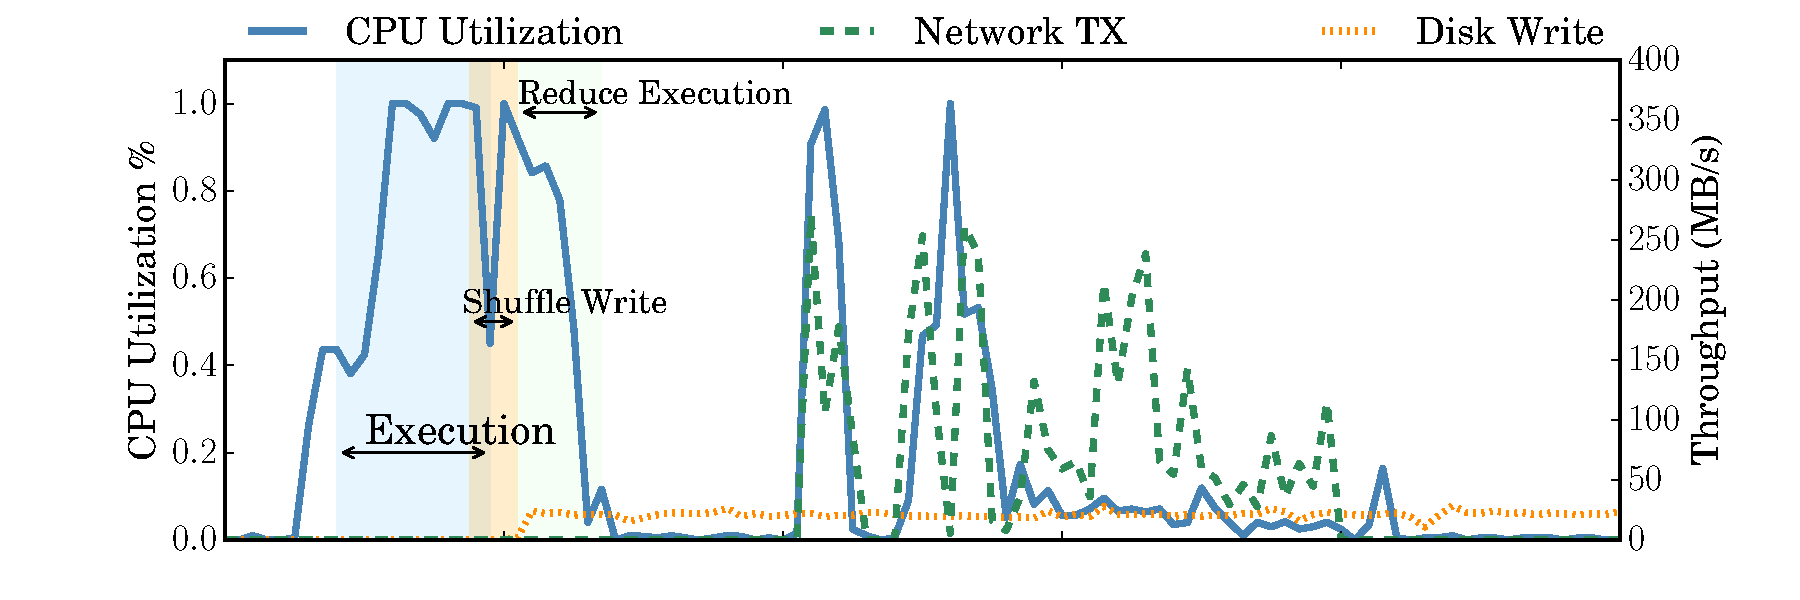
\includegraphics[width=\textwidth]{../../PPoPP-2018/fig/util.pdf}
	\bicaption[fig:util]{运行包含一个shuffle的Spark应用时的硬件资源利用率}{运行包含一个shuffle的Spark应用时的硬件资源利用率}{Fig}{CPU utilization and I/O throughput of a node
	during a Spark single shuffle application}
\end{figure}

\subsection{粗粒度的资源分配}

在现有的硬件资源分配机制下,当一个slot被计算框架分配给一个任务的时候,只有在该任务执行结束,这个slot以及其对应的硬件资源才会被释放。
对于一个map任务的结束是在他完成了shuffle write之后。
而在reduce任务一端,当一个reduce任务占用一个slot之后,它首先需要的只是通过一些I/O操作来获取远程的shuffle数据。
而在图\ref{fig:util}中,可以看到shuffle数据的写入和shuffle数据的读取都是I/O密集型操作,在这两个阶段,slot中的CPU利用率很低。
反过来,在进行计算的过程中,节点上的I/O资源则被大量闲置。
由此可知,在目前以Spark为代表的分布式DAG计算框架分配的任务的不同阶段对硬件资源的需求是不一致的。
但是当前这种主流的粗粒度资源分配方式为了满足任务在不同阶段的需求,只能舍弃一部分硬件资源的率用率。
因此要改变这种资源分配与需求的不匹配,必须提供一种更细粒度的资源分配机制。

\subsection{同步滞后的shuffle读取}

在目前的主流分布式DAG计算框架中,大多采用了Bulk Synchronous Parallel(BSP)模型来控制每个计算阶段。
因此当图\ref{fig:util}中的reduce阶段被调度时,集群中所有节点都会几乎同时启动reduce任务。
而reduce任务启动之后首先需要通过网络来完成shuffle数据的读取。
结合图\ref{fig:util}可以发现,在“shuffle read”阶段,该节点的网络产生了一个瞬时的流量高峰,而此时集群中其他节点也会产生相应的流量高峰。
这种几乎同时的流量高峰的出现,会对整个集群的网络带来巨大的压力,极易造成链路上的拥塞。
而当网络检测到拥塞时,无论是传统的TCP\cite{tcp}还是更先进的DCTCP\cite{dctcp}都会降低传输速率。
同时拥塞的发生还可能导致网络中交换机的丢包和TCP的重传等。
这些因素都会减慢shuffle读取时网络传输的速率,延长了shuffle读取过程,进而损害了reduce阶段的性能。

\subsection{低效率的磁盘操作}
\label{subsec:size}

在整个shuffle过程中,至少存在两次磁盘操作,即map阶段的shuffle数据写入磁盘和reduce阶段从远程磁盘读取shuffle数据。
在前文中提到的粗粒度的资源分配机制使得计算任务中的I/O操作会阻塞CPU内存等计算资源的释放和利用。
而其中低效率的磁盘操作更加剧了这个阻塞带来的延迟。

为了解决磁盘读写阻塞带来的延迟,首先需要回答两个问题:shuffle数据在磁盘的持久化是否必要?如果持久化是必要的,那么能否通过异步的方式来隐藏磁盘操作的开销?
对于将shuffle数据写入磁盘的必要性,在当下数据中心内存日益增大的背景下,为了节约内存而采用的将shuffle数据写入磁盘的方式(spill)并没有那么强的必要性。
而且相较于应用的输入数据而言,shuffle数据作为中间结果,其体积要相对小很多。
比如Spark Terasort\cite{spark-tera}中,shuffle数据只占到了输入数据的25\%不到。
在一些研究中\cite{makingsense}的数据也表明,shuffle数据大约只占到了输入数据的10\% $\sim$ 20\%。
从另一个角度来看,目前出现了越来越多的基于内存的分布式存储系统,比如memcached\cite{memcached},Tachyon\cite{tachyon}(现在的Alluxio\cite{alluxio})以及RAMCloud\cite{ramcloud}等。
这个趋势间接表面了在目前的数据中心环境下,内存资源是足够用来存放这些数据的。

退一步说,即使受限于内存体积,使得对shuffle数据的磁盘写操作不可避免,我们认为通过结合应用上下文的shuffle内存数据管理仍然可以很好的隐藏磁盘操作的开销。
由于DAG的存在,结合调度算法可以很容易就获取任务的调度顺序。
在这个前提下,即使内存资源十分紧张,shuffle的数据也可以通过异步预取的方式,提前从磁盘缓存在内存中。
因此我们认为,目前在shuffle过程中低效率的磁盘操作是可以被优化的。

\subsection{多轮任务执行}

在运行分布式DAG计算应用的时候,对于每一阶段的计算任务,无论是经验还是这些框架的手册都推荐在开发应用时将每个计算阶段并行的任务划分成多轮。
即对于一个有$s$个计算slot的计算集群而言,每个计算阶段的并行任务$t$:
\begin{equation}
	\label{eq:multi}
	t = k \times x \quad (k = 1, 2, 3, ...)
\end{equation}
比如Hadoop MapReduce的手册\cite{hadooptutorial}建议每个节点运行10-100个map任务(即等式\ref{eq:multi}中 $k \in [10, 100]$)。
同时该手册还建议运行时将任务的并发度调整到“$0.95$ 或 $1.75 \times$ 节点数 $\times$ 每个节点的最大容器数”。
Spark的配置手册\cite{sparkconf}也建议为节点上的每个CPU分配2-3个任务(即等式\ref{eq:multi}中 $k = 2, 3$)。

对于shuffle数据而言,当每一个map任务运行结束时,该任务所产生的shuffle数据就能被完整的获取。
与此同时,结合图\ref{fig:util},可以观察到在任务执行过程中,网络一直处于闲置状态。
因此在多轮任务执行的应用环境当中,如果shuffle传输的目的节点已知,那么shuffle数据便可以在map阶段的执行过程中进行预取。
这种多轮任务的属性则可以很好的将shuffle数据传输过程进行重叠,进而消除目前存在与reduce任务执行过程中的显示shuffle网络传输等待时间。

\section{本章小结}
通过以上的观察和分析,我们认为shuffle存在继续优化的空间。
具体来讲,就是通过解耦合的方式移除阻塞式的I/O操作,然后利用多轮任务执行的特性对shuffle数据进行预取,同时通过内存数据缓存和网络传输过程中的优化来进一步加速shuffle的读写。
基于上述优化目标,我们提出了SCache --- 针对分布式DAG计算框架shuffle过程的优化系统。
在图\ref{fig:workflow}的下半部分展现了DAG计算框架与SCache协同工作时的工作流程。
在“shuffle write”阶段,SCache通过内存拷贝的方式讲数据直接从任务的内存空间拷贝到预留的shuffle数据存储内存区域。
与此同时,磁盘的写操作将被省略。而由分布式DAG计算框架分配的slot资源也会在内存拷贝结束之后被立即释放。
这些缓存在内存中的shuffle数据会在SCache完成对reduce任务的预调度之后立刻进行网络传输。
这种数据预取方式既能将“shuffle read”阶段的时间很好的隐藏在map任务执行的过程中,又能避免传统BSP模型下,分布式DAG计算框架统一调度和执行reduce任务带来的同步瞬时大量的网络吞吐。

为了实现以上优化:
\begin{itemize}
	\item Shuffle的过程必须从计算任务中解耦,从而实现更细粒度的资源分配和更高的资源利用率。
	\item Reduce任务必须在map阶段就进行预调度,从而实现shuffle数据预取。同时在预调度的过程中不能真正启动reduce任务,以防其占用计算资源。
	\item 需要结合DAG计算逻辑实现精细化shuffle数据内存缓存管理,进一步加快shuffle读写速度。
	\item 为了实现跨框架的优化方案,shuffle过程必须被独立到计算框架外部进行管理,并且实现一个具有通用性的API。
\end{itemize}

\section{Shuffle Optimization}
In this section, we present the detailed methodologies to achieve three design goals. The memory copy is used to decouple shuffle from execution. Shuffle data is pre-fetched without tasks launching with the heuristic MinHeap pre-scheduling scheme. And all shuffle data is managed outside DAG framework by SCache to provide a universal cross-framework optimization.
We choose Spark \cite{apachespark} as the representative of DAG computing framework to implement our optimization.

\begin{figure}
	\centering
	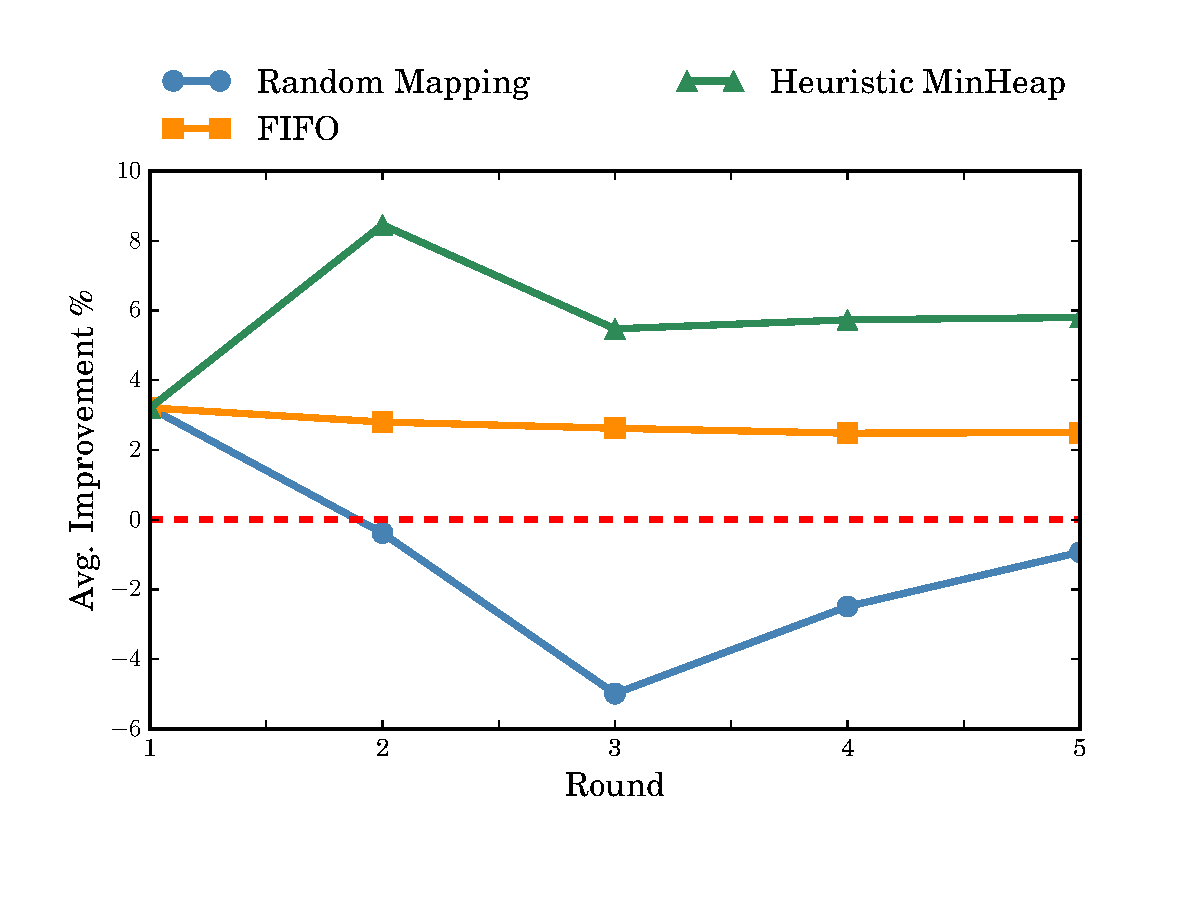
\includegraphics[width=0.9\linewidth]{fig/sim}
	\caption{Stage Completion Time Improvement of OpenCloud Trace}
	\label{fig:sim}
\end{figure}

\subsection{Decouple Shuffle from Execution}
In map tasks the partitioner takes a set of key-value pairs as input and calculates the partition number of a key-value pair by applying pre-defined the partition function to the key. After that, it stores the key-value pair in the corresponding data blocks. Each of the block contains the key-value pairs for one reduce partition. At last, blocks will be flushed to disk. The decoupling starts before data flushing. To avoid blocking the slot by disk write, we use memory copy to hijack shuffle data from Spark executor's JVM space. By doing this, a slot can be released as soon as it finishes CPU intensive computing. The pre-scheduling and pre-fetch starts when the collected shuffle data exceeds the threshold.

On the reduce side, shuffle read is decoupled by pre-fetching shuffle data to local SCache client after pre-scheduling before reduce tasks start.

To this end, all I/O operations are managed outside of the DAG framework, and the slot is occupied only by the CPU intensive phases of task.

\begin{figure}
	\centering
	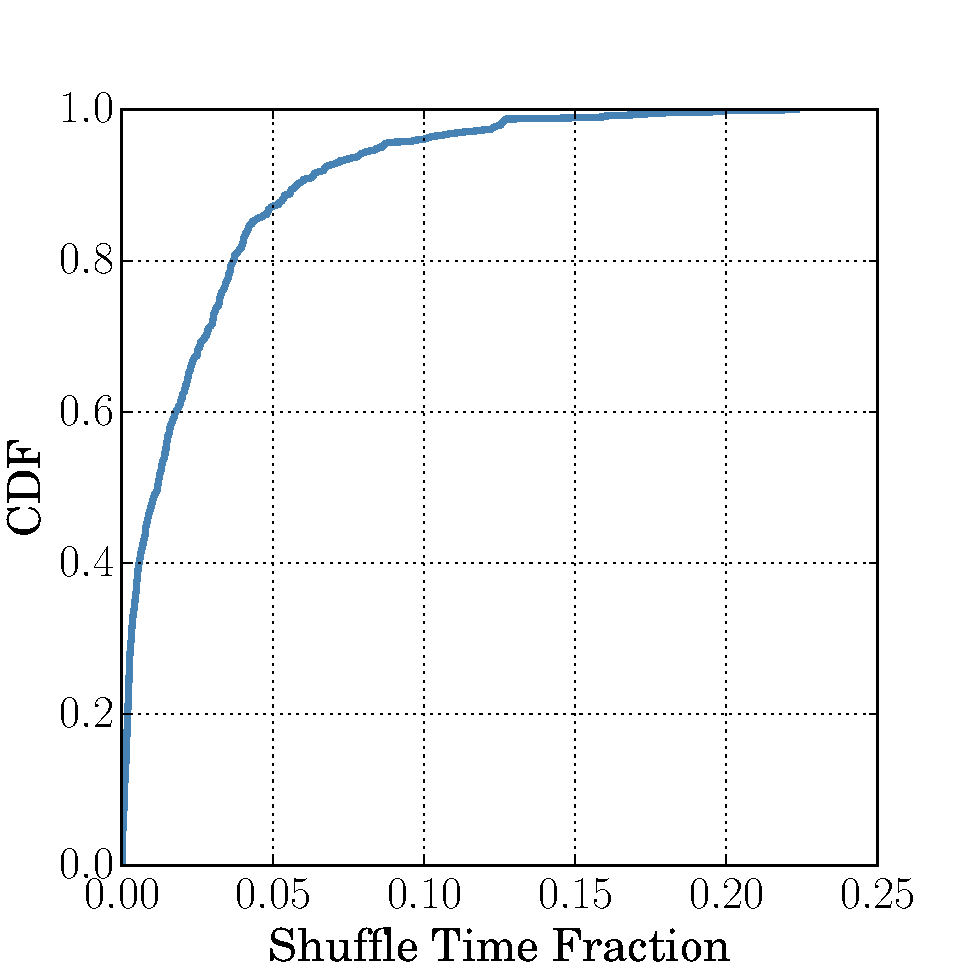
\includegraphics[width=0.75\linewidth]{fig/reduce_cdf}
	\caption{Shuffle Time Fraction CDF of OpenCloud Trace}
	\label{fig:cdf}
\end{figure}

\subsection{Pre-schedule with Application Context}
The main challenge toward the optimization is how to pre-schedule the reduce tasks without launching. The task --- node mapping is not determined until tasks are scheduled by scheduler of DAG framework. But as soon as they are scheduled, slots will be occupied to launch them. On the other hand, shuffle data cannot be pre-fetched without knowing the task --- node mapping.
To get rid of this dilemma, we propose a co-scheduling scheme. That is, the task --- node mapping is established ahead of DAG framework scheduler, and then enforce the mapping results to DAG scheduler while doing the real scheduling.

We use traces from OpenCloud \cite{opencloudtrace} for the simulation to evaluate the impact of different pre-scheduling schemes. The baseline (red dot line in Figure \ref{fig:sim}) is the stage completion time under Spark default scheduling algorithm. And then we remove the shuffle read time of each task, and do the simulation under three different schemes: random mapping, Spark FIFO, and our heuristic MinHeap.

% We explore several pre-scheduling schemes in different scenarios, and evaluate the performance calculating the improvement of reduce tasks completion time with trace of OpenCloud \cite{opencloudtrace}. We first emulate the scheduling algorithm of Spark to schedule the reduce tasks of one job, and take the bottleneck of the task set as the completion time. Then we remove the shuffle read time as the assumption of shuffle data pre-fetch and emulate under different schemes. The result is shown in \ref{fig:sim}.
% \begin{figure*}
% 	\centering
% 	\begin{minipage}{0.34\linewidth}
% 		\begin{figure}[H]
% 			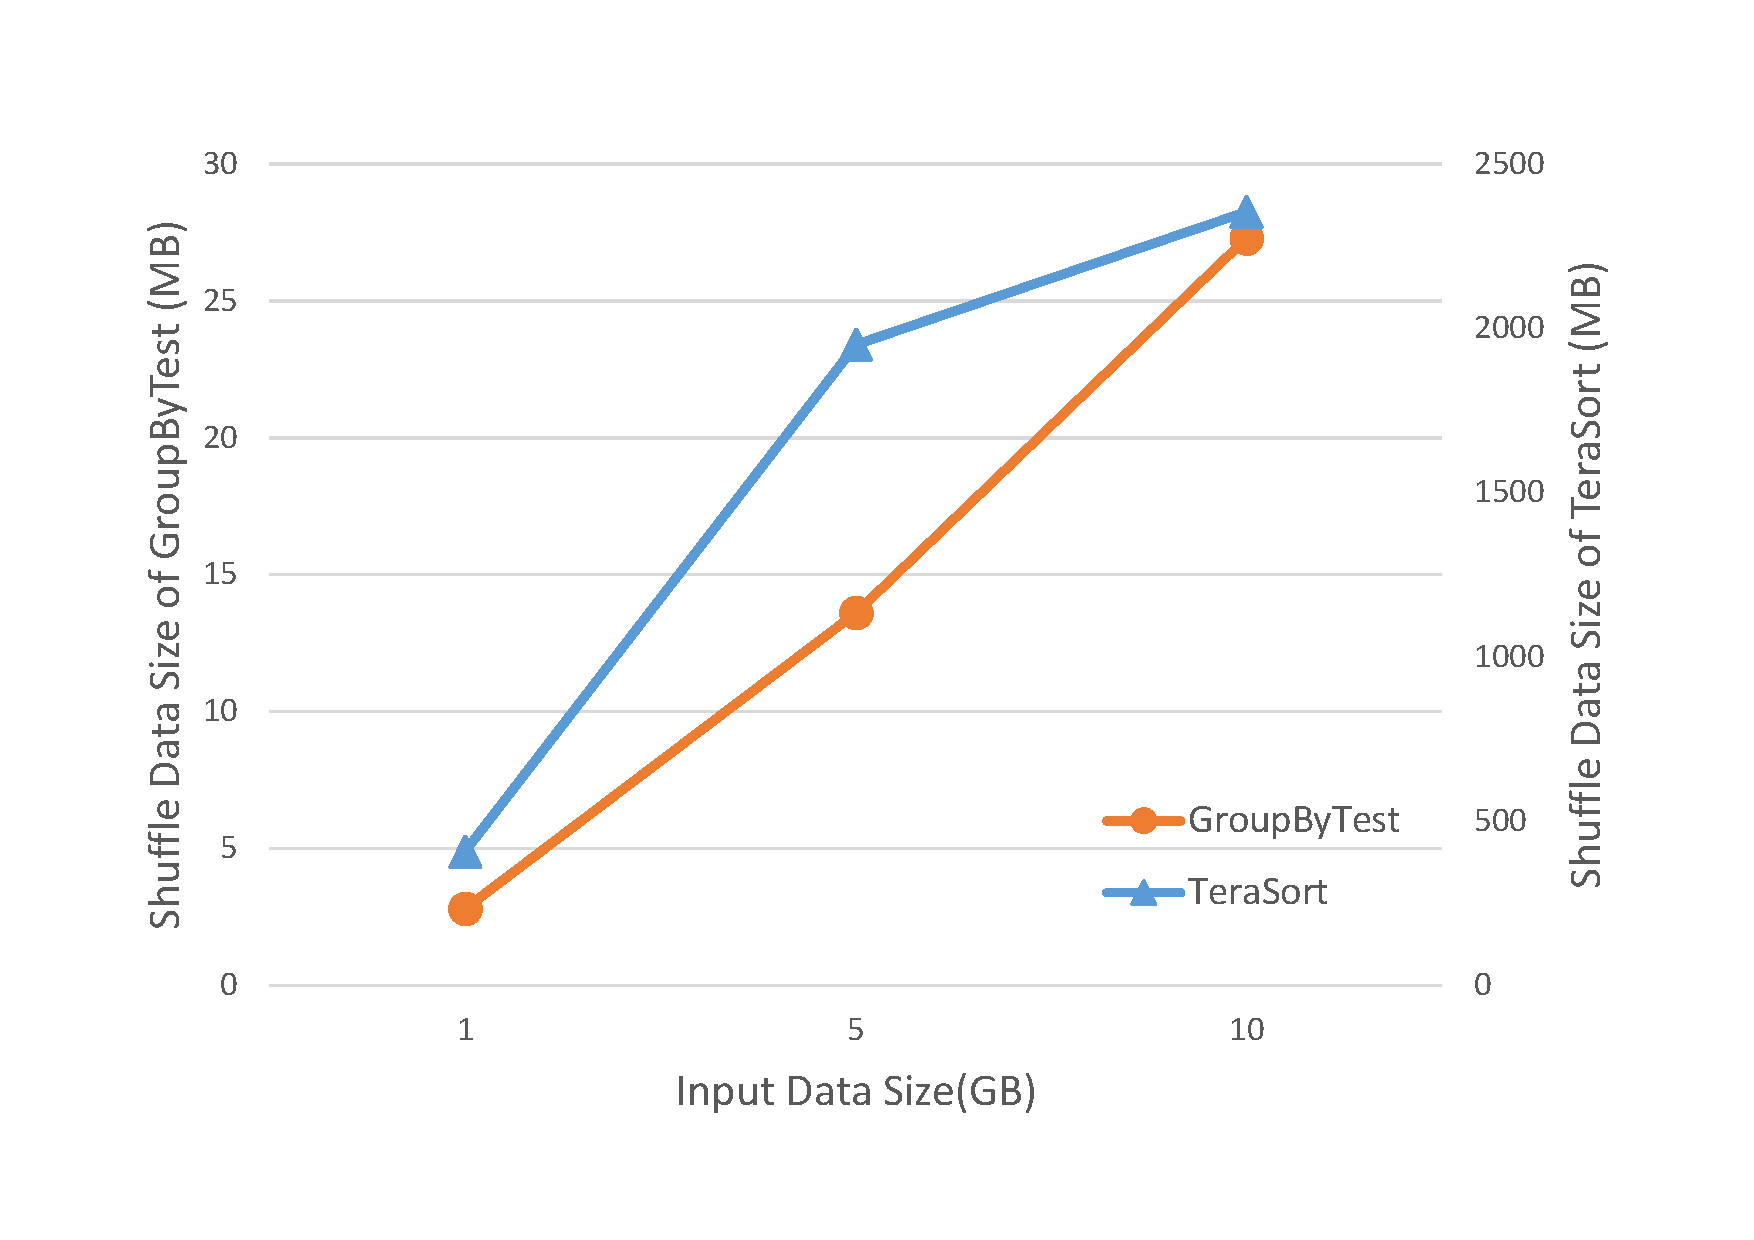
\includegraphics[width=\textwidth]{fig/shuffle_size}
% 			\caption{Shuffle Size Comparing with Input Size}
% 			\label{fig:shuffle_size}
% 		\end{figure}
% 	\end{minipage}
% 	\begin{minipage}{0.65\linewidth}
% 		\begin{figure}[H]
% 			\begin{subfigure}{0.5\textwidth}
% 				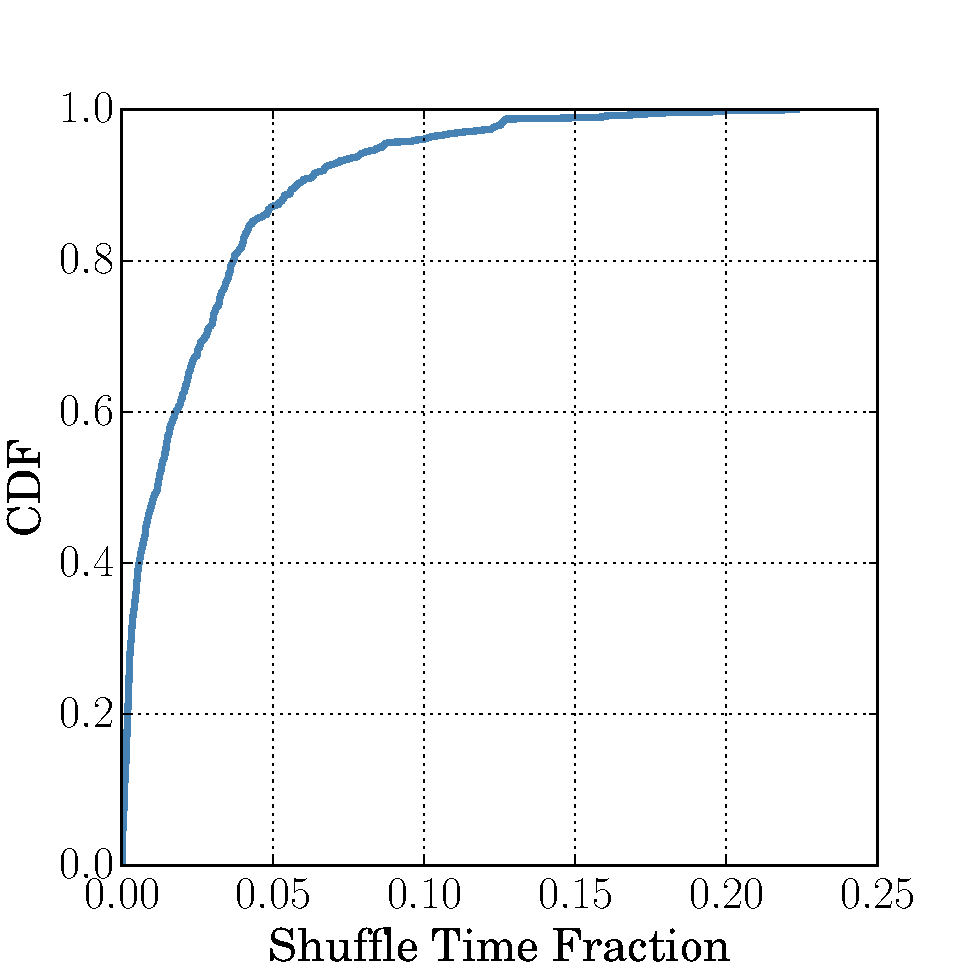
\includegraphics[width=\linewidth]{fig/reduce_cdf}
% 				\caption{Shuffle Time Fraction CDF}
% 				\label{fig:cdf}
% 			\end{subfigure}	
% 			\begin{subfigure}{0.5\textwidth}
% 				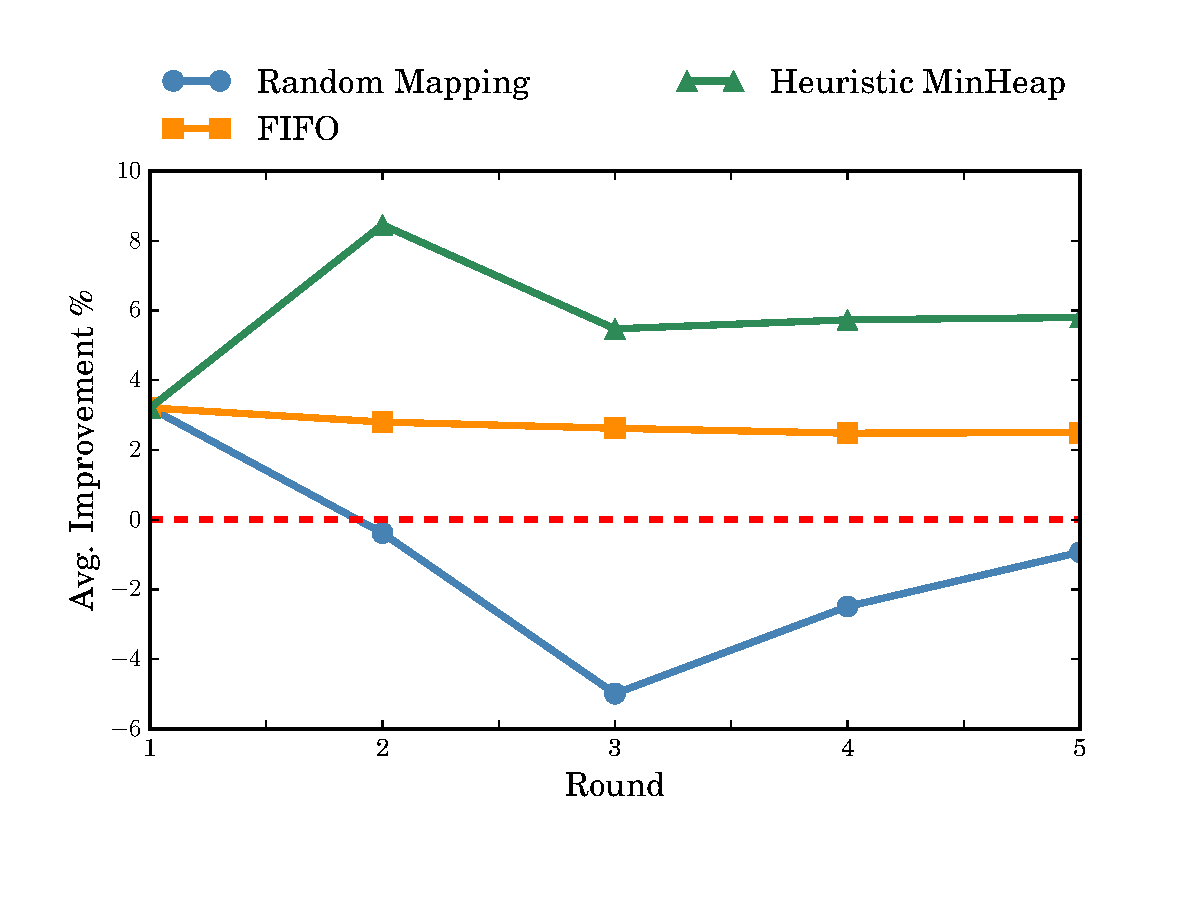
\includegraphics[width=\linewidth]{fig/sim}
% 				\caption{Stage Completion Time Improvement}
% 				\label{fig:sim}
% 			\end{subfigure}	
% 			\caption{Emulate Result of OpenCloud Trace}
% 		\end{figure}
% 	\end{minipage}
% \end{figure*}
% \begin{figure}



Note that most of the traces from OpenCloud is shuffle-light workload as shown in Figure \ref{fig:cdf}. The average shuffle read time is 2.3\% of total reduce completion time.

\subsubsection{Failure of Random Mapping}\label{randomassign}
The simplest way of pre-scheduling is mapping tasks to different nodes randomly. It only guarantees that each node run same number of tasks. As shown in Figure \ref{fig:sim}, Random mapping works well when there is only one round of tasks. But the performance collapses as the round number grows. It is because that data skew commonly exists in data-parallel computing \cite{skewtune, reining, gufler2012load}. Several heavy tasks might be assigned on the same node. This collision then slows down the whole stage and makes the performance even worse than the baseline. In addition, randomly assigned tasks also ignore the data locality between shuffle map output and shuffle reduce input, which might introduce extra network traffic in cluster.


\subsubsection{Shuffle Output Prediction}\label{shuffleprediction}
The failure of random mapping was obviously caused by application context (e.g. shuffle data size) unawareness. Note that the optimal schedule decision can be made under the awareness of shuffle dependencies number, partition number and shuffle size for each partition. The first two of them can be easily extracted from DAG information. To achieve a better scheduling result, the shuffle size for each partition should be predicted during the initial phase of map tasks.

According to the DAG computing process, the shuffle size of each reduce task is decided by input data, map task computation, and hash partitioner. Each map task produces a data block for each reduce task. The size of each reduce partition can be calculated $reduceSize_i = \sum_{j=0}^{m} {BlockSize_{ji}}$ ($m$ is the number of map tasks). $BlockSize_{ji}$ represents the size of block which is produced by map $task_j$ for reduce $task_i$ (e.g., block `1-1' in Figure \ref{fig:shuffle}).

For Hadoop MapReduce, the $BlockSize_{ji}$ can be predicted with decent accuracy by liner regression model based on observation that the ratio of map output size and input size is invariant given the same job configuration \cite{ishuffle, predict}.

But the sophisticated DAG computing framework like Spark introduces more uncertainties. For instance, the reduce stage in Spark has more tasks than Hadoop MapReduce. More importantly, the customized partitioner might bring huge inconsistency between observed map output blocks distribution and the final reduce input distribution as presented in Figure \ref{fig:dis}. We use different datasets with different partitioners and normalize three sets of data to $0-1$ to fit in one figure. In Figure \ref{fig:hash_pre}, we use a random input dataset with the hash partitioner. In Figure \ref{fig:range_pre_sample}, we use a skew dataset with the range partitioner of Spark \cite{sparksource}.
The observed map outputs are randomly picked. As we can see, in hash partitioner, the distribution of observed map output is close to the final reduce input distribution. The prediction results also turn out to be good. However, the huge inconsistency between final reduce distribution and observed distribution results in a deviation in linear regression model.
% Several map outputs (marked as Map Output in Figure \ref{fig:shuffle}) are picked as observation objects to train the model and than predict the final reduce distribution.

\begin{equation}
\label{equationsample}
\begin{aligned}
	BlockSize_{ji} &= {{InputSize_j \times \frac{sample_i}{s \times p}}} \\
	sample_i &= \text{number of samples for $reduce_i$}
\end{aligned}
\end{equation}

To handle this inconsistency, we introduce another methodology named weighted reservoir sampling. The classic reservoir sampling is designed for randomly choosing \textit{k} samples from \textit{n} items, where \textit{n} is either a very large or an unknown number \cite{reservoir}. For each partition of map task, we use reservoir sampling to randomly pick $s \times p$ of samples, where $p$ is the number of reduce tasks and $s$ is a tunable number. The number of input data partition and reduce tasks can be easily obtained from the DAG information. In Figure \ref{fig:range_pre_sample}, we set $s$ equals $3$. After that, the map function is called locally to process the sampled data (\textit{sampling} in Figure \ref{fig:shuffle}). The final sampling outputs are collected with the input size of each map partition which is used as weight for each set of sample.

As we can see in Figure \ref{fig:range_pre_sample}, the result of sampling prediction is much better even in a very skew scenario. The variance of the normalized between sampling prediction and reduce distribution is because the standard deviation of the prediction result is relatively small compared to the average prediction size, which is $0.0015$ in this example. Figure \ref{fig:prediction_relative_error} further proves that the sampling prediction can provide precise result even in the dimension of absolute shuffle partition size. On the opposite, the result of linear regression comes out with huge relative error.

However, sampling prediction trade accuracy with extra overhead in DAG computing process. Though in most cases, the overhead is acceptable, the sampling prediction will be triggered only when the range partitioner or customized non-hash partitioner occurs. We will show the overhead in the Section \ref{evaluation}.

During the phase of shuffle output prediction, the composition of each reduce partition is calculated as well. We define $prob_i$ as

\begin{equation}
\label{equationprob}
\begin{aligned}
	prob_i &= \max_{0 \leq j \leq m} \frac{BlockSize_{ji}}{reduceSize_i} \\
    m &= \text{number of map tasks}
\end{aligned}
\end{equation}

This parameter is used to achieve a better locality while performing shuffle scheduling.

\subsubsection{Heuristic MinHeap Scheduling}\label{h-minheap}
In order to achieve the uniform load on each node while reducing the network traffic, we present a heuristic MinHeap scheduling algorithm (\ref{hminheap}) for single shuffle.  
As for the input of $SCHEDULE$ function in Algorithm \ref{hminheap}, $m$ is the partition number of input data; $h$ is the array of nodes ID in cluster; $p\_reduces$ is the predicted reduce matrix. Each row in $p\_reduces$ contains $rid$ as reduce partition ID; $size$ as predicted size of this partition; $prob$ as the maximum composition portion of reduce data; $host\_id$ as the node ID that produces the maximum portion of reduce data, and $assigned\_id$ as the node ID assigned by Algorithm \ref{hminheap}. As for $M$, it is consists $host\_id$, an array of $reduce$ scheduled on this node and the $size$ of them.

\begin{minipage}{\columnwidth}
\begin{algorithm}[H]
\caption{Heuristic MinHeap Scheduling for Single Shuffle}
\label{hminheap}
	\begin{algorithmic}[1]
	\small
	\Procedure{schedule}{$m, h, p\_reduces$}
		\State $R\gets$ sort $p\_reduces$ by size in descending order
		\State $M\gets$ min-heap $\left\{ host\_id \rightarrow \left( \left[ reduces \right], size \right) \right\}$
		\State $idx\gets$ len$\left(R\right) - 1$
		\While{$idx \geq 0$}
		\Comment{Schedule reduces by MinHeap}
		\State $M\left[0\right].size \mathrel{+}= R\left[idx\right].size$
		\State $M\left[0\right].reduces.append\left(R\left[idx\right]\right)$
		\State $R\left[idx\right].assigned\_host \gets M \left[0\right].host\_id$
		\State Sift down $M\left[0\right]$ by $size$
		\State $idx\gets idx-1$
		\EndWhile
		\State $max\gets$ maximum size in $M$
		\State Convert $M$ to mapping $\left\{ host\_id \rightarrow \left( \left[ rid\_arr \right], size \right) \right\}$
		\ForAll{$reduce$ in $R$}
		\Comment{Heuristic swap by locality}
			\If{$reduce.assigned\_id \neq reduce.host\_id$}
				\State $p\gets reduce.prob$
				\State $norm\gets \left(p-1/m\right)/\left(1-1/m\right)/10$
				\State $upper\_bound \gets \left(1 + norm\right) \times max$
				\State SWAP\_TASKS$\left(M, reduce, upper\_bound\right)$
			\EndIf
		\EndFor
		% \Comment{$m$ is the number of input data}
		% \Comment{$r$ is partition number of reduces}
		% \Comment{$hosts$ is array of (hostid, partitionids[], size)}
		% \Comment{$c$ is $r*m$ array of composition data}
		% \Comment{$pSize$ is $r$ size array of predicted size of reduces}
		\Return $M$
	\EndProcedure
	\Procedure{swap\_tasks}{$M, reduce, upper\_bound$}
		\State $reduces \gets M\left[reduce.host\_id\right].reduce$	
		\State $candidates \gets$ Select from $reduces$ that $assigned\_id \neq host\_id$ \textbf{and} total size closest to $reduce.size$
		\State $\Delta size \gets sizeOf\left(candidates\right) - reduce.size$
		\State $size\_host \gets M\left[reduce.host\_id\right].size - \Delta size$
		\State $size\_assigned \gets M\left[reduce.assigned\_id\right].size + \Delta size$
		\If{$size\_host\leq upper\_bound$ \textbf{and} \\
			\qquad \; $size\_assigned\leq upper\_bound$}
			\State Swap $candidates$ and $reduce$
			\State Update $size$ in $M$
			\State Update $assigned\_host$ in $candidates$ and $reduce$
		\EndIf
	\EndProcedure
	\end{algorithmic}
\end{algorithm}
\end{minipage}


This algorithm can be divided into two rounds. In the first round (i.e., the first $while$ in $SCHEDULE$), the reduce tasks are first sorted by size in a descending order. For hosts, we use a min-heap to maintain the priority by size of assigned tasks. So that the tasks can be distributed evenly in the cluster.
% After the scheduling, the completion time of reduce stage is close to the optimal. \textcolor{red}{may need to add math prove between this and optimal}.
In the second round, the task --- node mapping will be adjusted according to the locality. 
The $SWAP_TASKS$ will only be trigged when the $host\_id$ of a reduce task is not equal the $assigned\_id$.
The closer $prob$ is to $1/m$, the more evenly this reduce partition is produced in cluster. For a task which contains at most $prob$ data from $host$, the normalized probability $norm$ is calculated as a bound of performance degradation. We set the $upper\_bound$ of performance degradation to be the 10\% slower than the origin (in extreme skew scenarios). This normalization can ensure that more performance would be traded when the locality level increases. 
Inside the $SWAP\_TASKS$, tasks will be selected and swapped without exceeding the $upper\_bound$ of each host. 
Unlike the na\"{i}ve Spark scheduling algorithm, these information helps the scheduler make a more balanced task --- node mapping, which accelerates the reduce stage. This is the by-product optimization harvested from shuffle size prediction.

We use the OpenCloud \cite{opencloudtrace} trace to evaluate Heuristic MinHeap. Without swapping, the Heuristic MinHeap can achieve a better performance improvement (average 5.7\%) than the default Spark FIFO scheduling algorithm (average 2.7\%).

% In the case of extreme skew scenario, such as Figure \ref{fig:range_pre_sample}, Heuristic MinHeap trades about 0.05\% percent of stage completion time for 99\% reduction of shuffle data transmission through network by heuristicly swapping tasks.

\begin{figure}
	\centering
	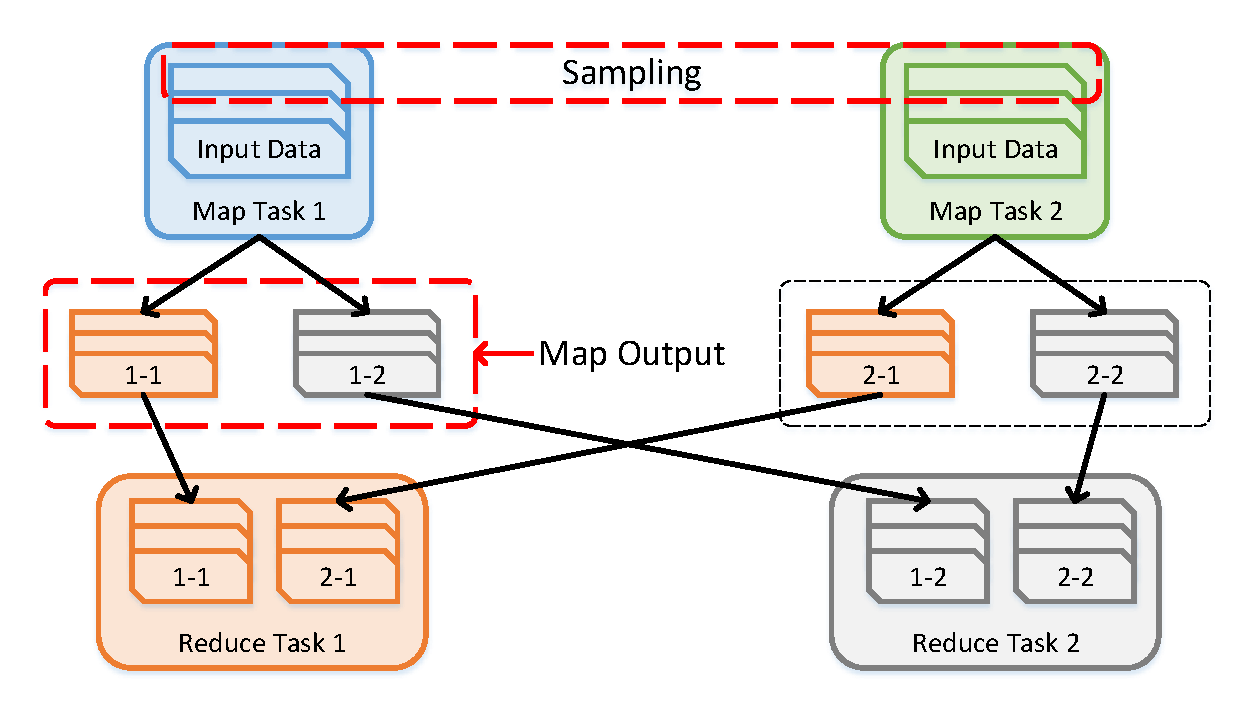
\includegraphics[width=0.9\linewidth]{fig/shuffle}
	\caption{Shuffle Data Prediction}
	\label{fig:shuffle}
\end{figure}

\begin{figure*}
	\centering
	\begin{subfigure}[b]{0.32\linewidth}
		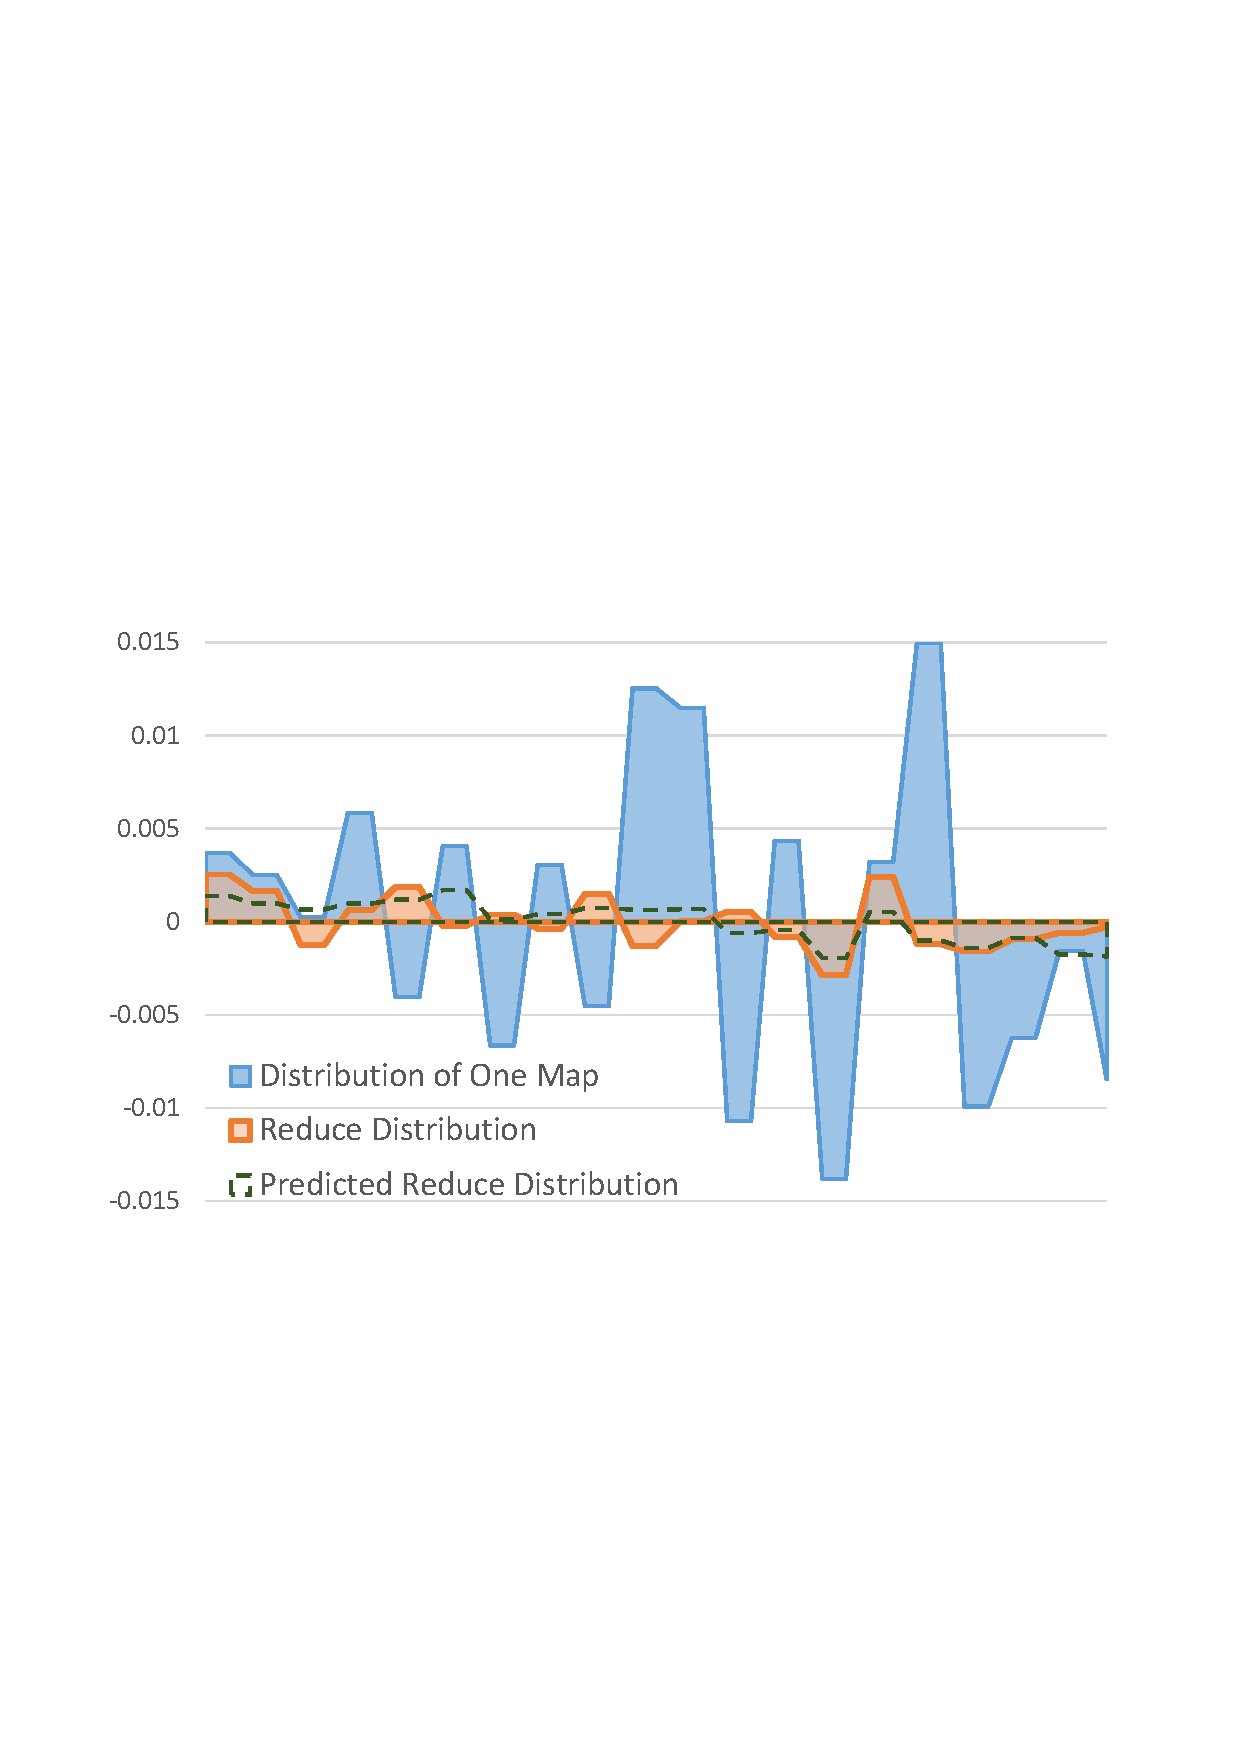
\includegraphics[width=\linewidth]{fig/hash_pre}
		\caption{Linear Regression Prediction of Hash Partitioner}
		\label{fig:hash_pre}
	\end{subfigure}
	\begin{subfigure}[b]{0.32\linewidth}
		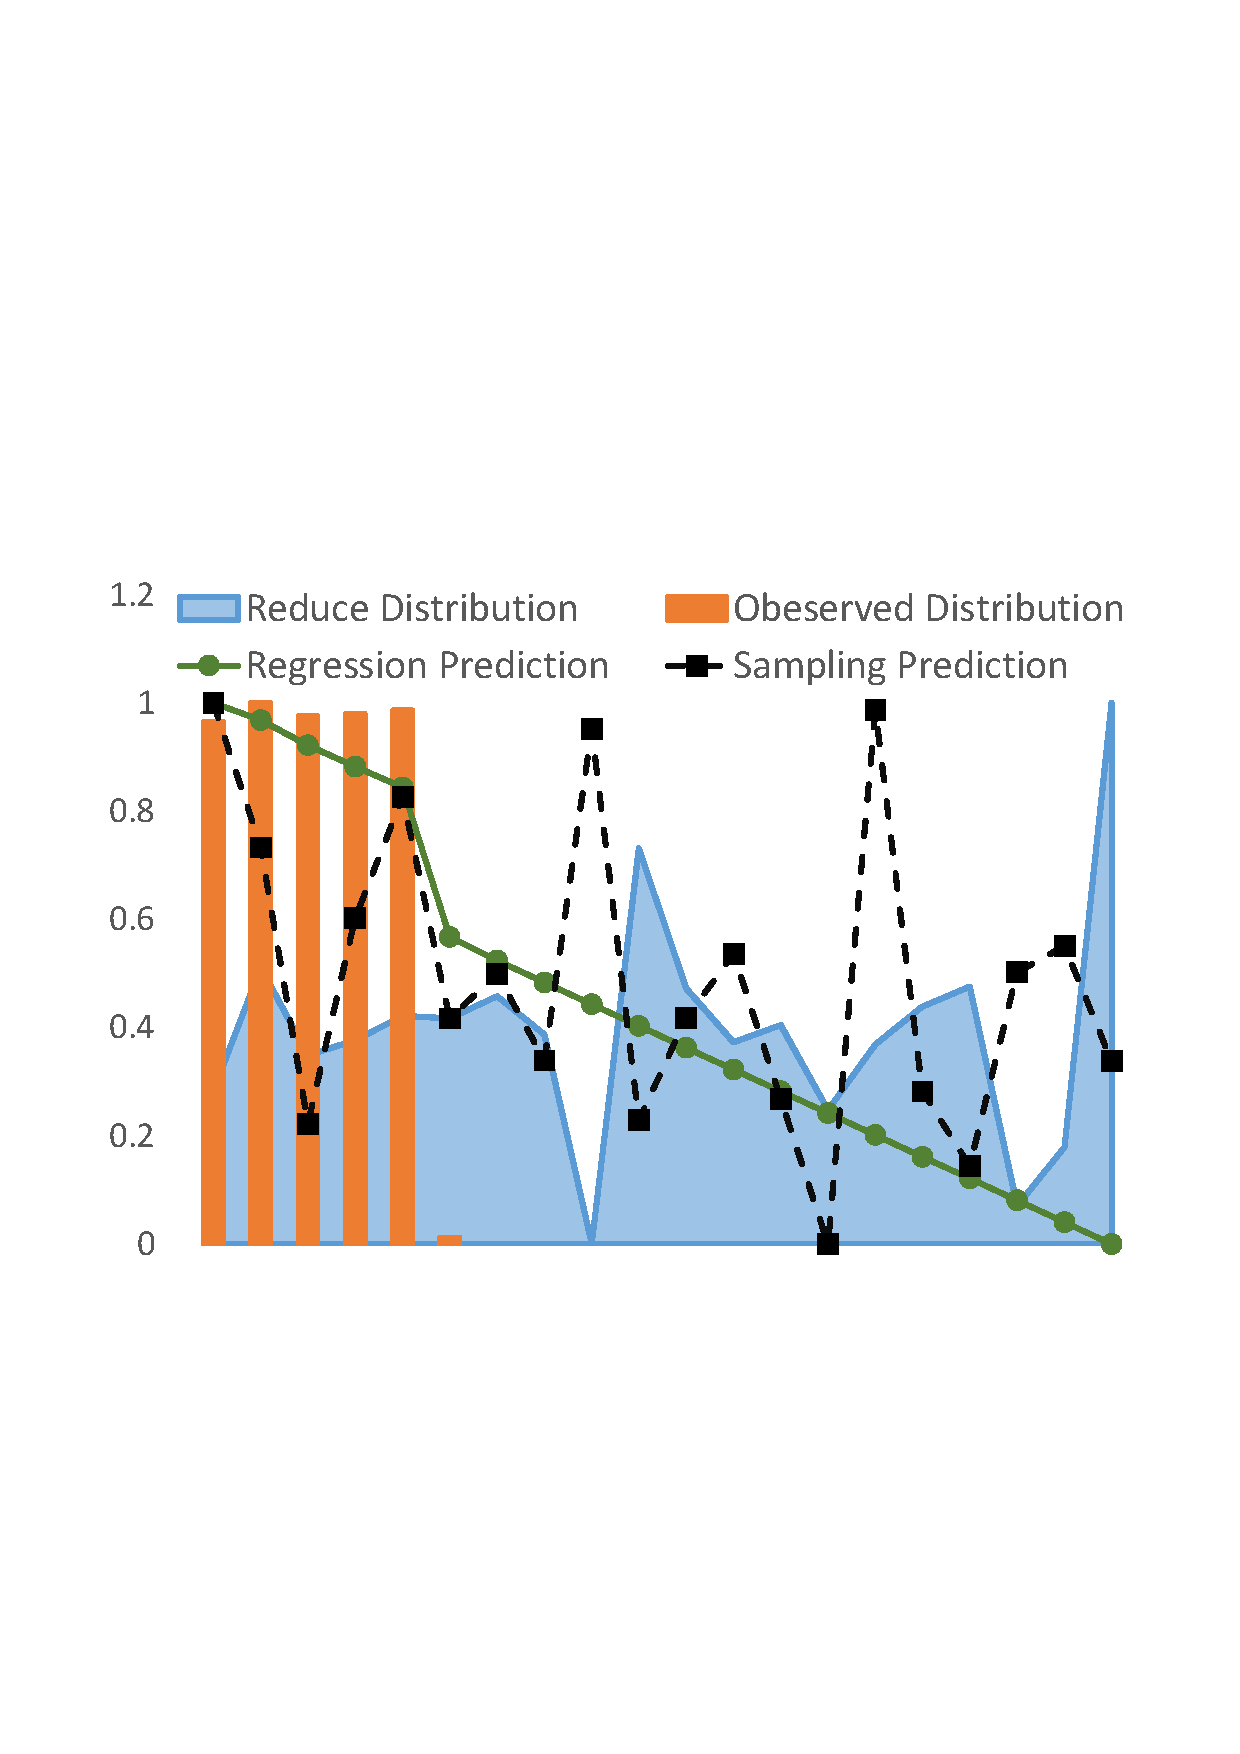
\includegraphics[width=\linewidth]{fig/range_pre_sample}
		\caption{Linear Regression and Sampling Prediction of Range Partitioner}
		\label{fig:range_pre_sample}
	\end{subfigure}
	\begin{subfigure}[b]{0.32\linewidth}
		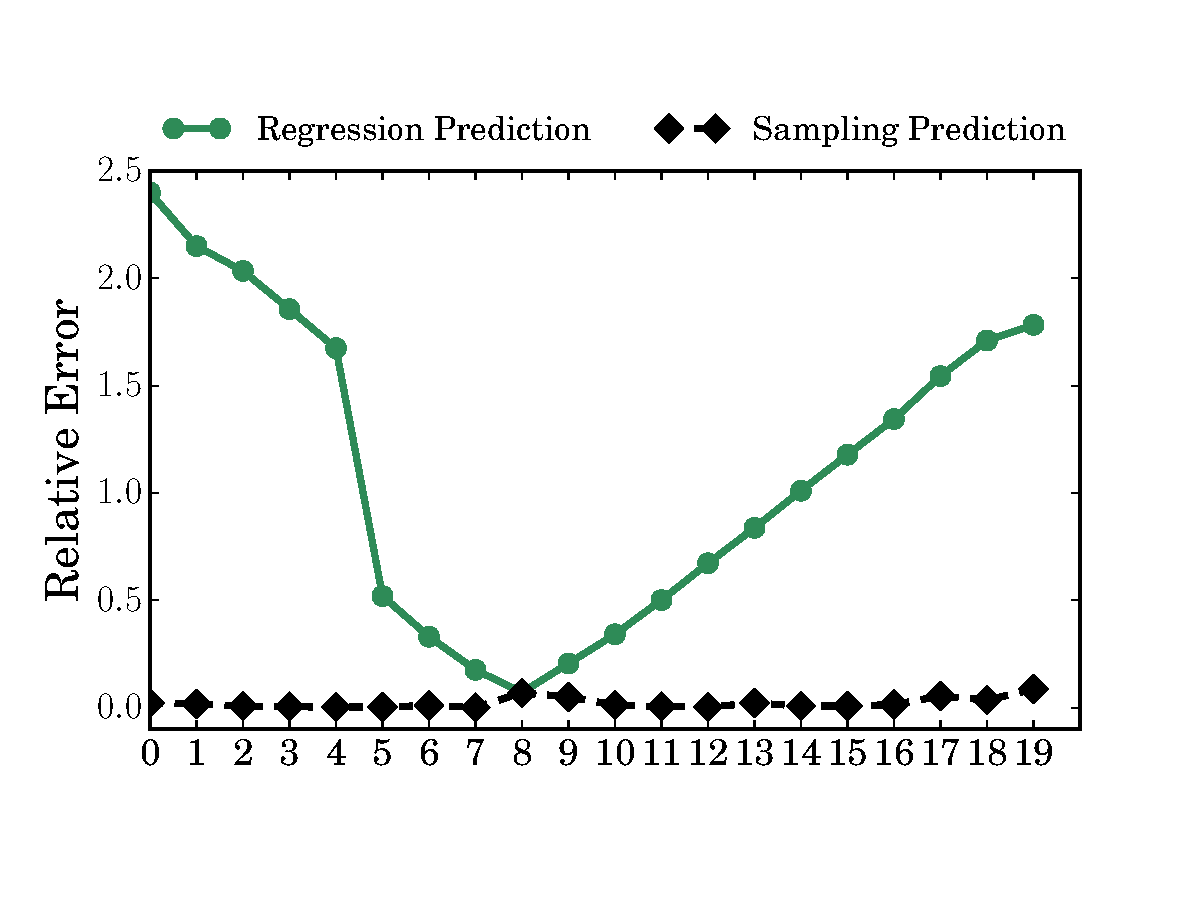
\includegraphics[width=\linewidth]{fig/prediction_relative_error}
		\caption{Prediction Relative Error of Range Partitioner}
		\label{fig:prediction_relative_error}
	\end{subfigure}
	\caption{Reduction Distribution Prediction}
	\label{fig:dis}
\end{figure*}

\subsubsection{Cope with Multiple Shuffles}
Unlike Hadoop MapReduce, multiple shuffles commonly exist in DAG computing. The techniques mentioned in Section \ref{shuffleprediction} can only handle the ongoing shuffle. For those pending shuffles, it's impossible to predict the sizes. Let all map tasks of shuffle to be scheduled by DAG framework simultaneously can relieve the dilemma. But doing this introduces extreme overhead such as extra task serialization. To avoid violating the optimization from framework, we present Algorithm \ref{mhminheap} to cope with multiple shuffles.

As illustrated in pseudo code \ref{mhminheap}, the size of reduce on each node of previously scheduled $shuffles$ are counted. When a new shuffle starts, the $mSchedule$ is called to schedule the new one with previous $shuffles$. The $size$ of each reduce and its corresponding $porb$ and $host$ are updated by adding $p\_reduces$ of the new shuffle. Then the $schedule$ is called to perform the shuffle scheduling. When the new task --- node mapping is available, for each reduce task, if the new $assigend\_host$ of a reduce does not equal to the original one, the re-shuffle will be triggered to transfer data to new host for further computing. This re-shuffle is rare since the previously shuffled data in a reduce partition contributes a huge composition. It means in the schedule phase, the $SWAP\_TASKS$ can help revise the scheduling to match the previous mapping in $shuffles$ as much as possible while maintaining the good load balance.

\begin{minipage}{\columnwidth}
\begin{algorithm}[H]
\caption{Accumulate Scheduling for Multi-Shuffles}
\label{mhminheap}
	\begin{algorithmic}[1]
	\small
	\Procedure{mSchedule}{$m, h, p\_reduces, shuffles$}
		\State
		\Comment $shuffles$ is the previous array of $reduces$ 
		\ForAll{$r$ in $p\_reduces$}
			\State $r.size \mathrel{+}= shuffles\left[r.rid\right].size$
			\If{$shuffles\left[r.rid\right].size\geq r.size \times r.prob$}
				\State $r.prob\gets shuffles\left[r.rid\right].size / r.size$
				\State $r.host\_id\gets shuffles\left[r.rid\right].assigned\_host$
			\EndIf
		\EndFor
		\State $M\gets$ $SCHEDULE\left(m, h, p\_reduces\right)$
		\ForAll{$host\_id$ in $M$}
			\Comment Re-shuffle
			\ForAll{$r$ in $M\left[host\_id\right].reduces$}
				\If{$host\neq shuffles\left[r.rid\right].assigned\_host$}
				\State Re-shuffle data to $host$
				\State $shuffles\left[r.rid\right].assigned\_host\gets host$
				\EndIf
			\EndFor
		\EndFor
		\Return $M$
	\EndProcedure
	\end{algorithmic}
\end{algorithm}
\end{minipage} 
%# -*- coding: utf-8-unix -*-
%%==================================================
%% chapter02.tex for SJTU Master Thesis
%%==================================================

\chapter{SCache的实现}
\label{chap:impl}

本章将展现SCache系统的实现概况。
SCache是一个用Java和Scala语言开发的,开源的shuffle数据管理系统,并且提供了一个对于DAG任务预调度的附属调度器。
同时SCache还在设计时提供了跨框架的接口,来实现对于现有主流分布式DAG计算框架的shuffle优化。
在这次实现中,我们以Spark作为DAG计算框架的实例来阐述在SCache辅助下分布式DAG计算框架的新的计算流程。
我们首先在章节\ref{sec:overview}中介绍了系统设计的概要。
之后的章节分别介绍水塘采样算法,SCache在容错性上的取舍,以及计算框架在适配SCache时的工程上的开销和可行性分析。

\section{系统设计概要}
\label{sec:overview}

SCache在系统层面上主要包含三个部件:一个分布式的shuffle数据管理系统,一个DAG的附属调度器,和一个Spark系统内部的守护进程。
如图\ref{fig:arch}所示,SCache采用了类似于GFS\cite{gfs}经典的主从节点架构来实现对shuffle数据在集群中的管理。

\begin{figure}[!htp]
	\centering
	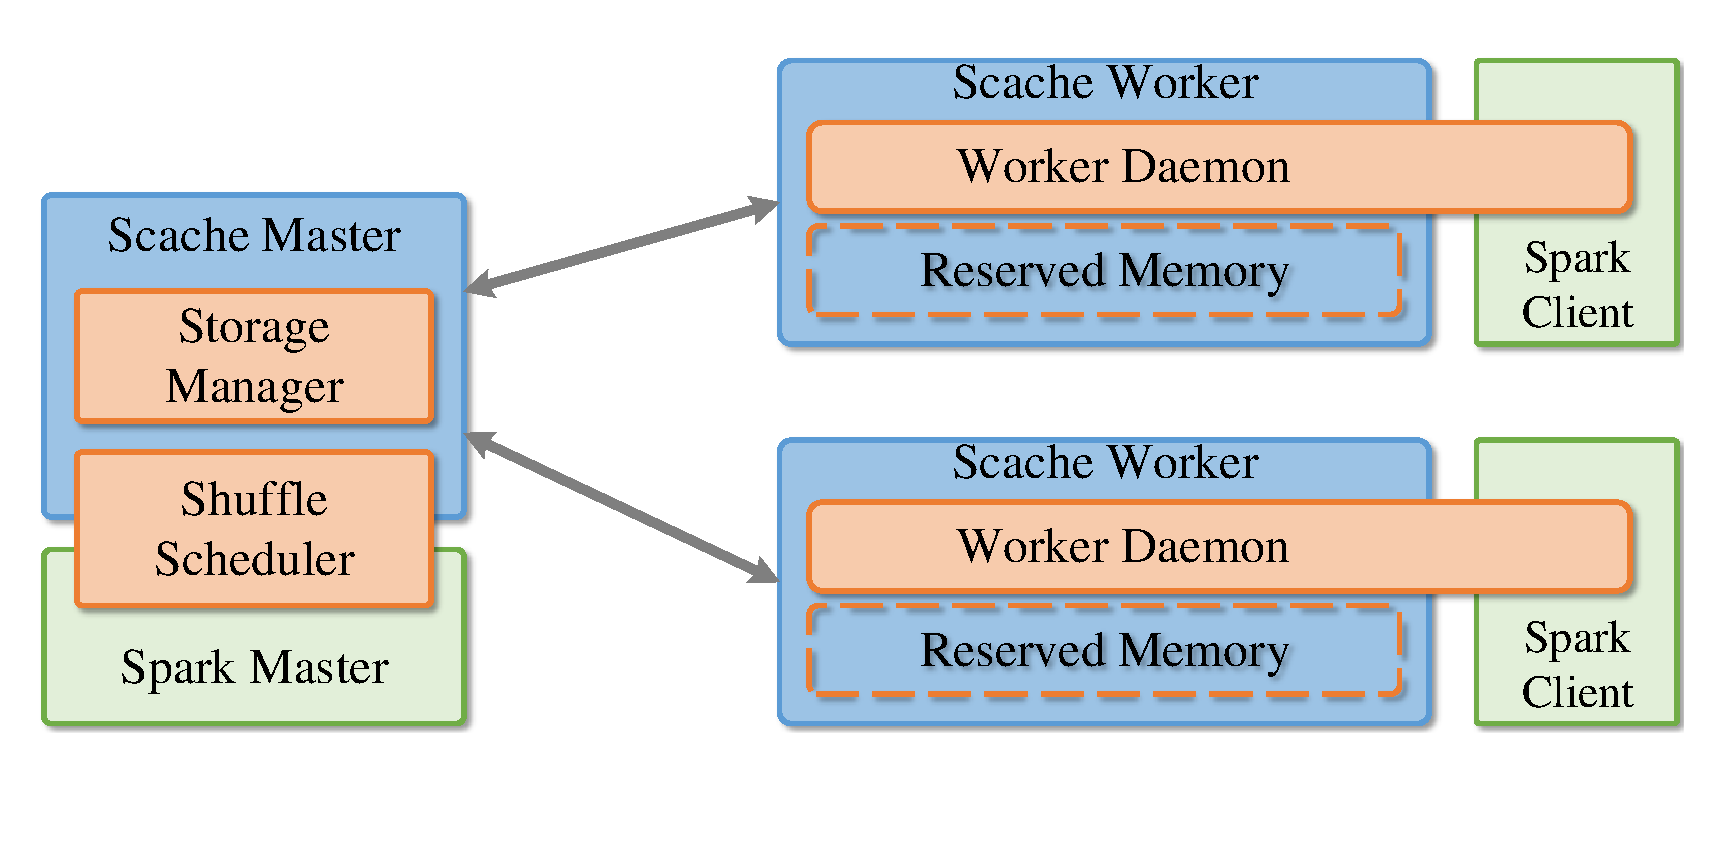
\includegraphics[width=0.8\textwidth]{../../PPoPP-2018/fig/arch.pdf}
	\bicaption[fig:arch]{SCache系统架构示意图}{SCache系统架构示意图}{Fig}{SCache Architecture}
\end{figure}

SCache的主节点负责管理整个分布式系统中的shuffle数据块预取与内存管理。
SCache的主节点中包含了DAG附属调度器,并且通过DAG附属调度器获取Spark上连接shuffle的reduce阶段任务预调度信息,任务的预调度执行顺序等。
此后SCache的主节点会将reduce阶段任务的预调度信息通知到各个从属工作节点。
当工作节点收到任务预调度信息之后,会立刻开始对远程已经完成的map任务进行shuffle数据的预取。
并且对于未完成的map任务,一旦工作节点通过内存拷贝的方式获取了相应的shuffle数据后就立即广播给集群中的各个节点,以便其开始shuffle的预取。
除此之外,SCache主节点还会根据任务的执行顺序信息给各个shuffle的数据单元标注上优先级并且发送给各个工作节点。

SCache的工作节点会在本地占用一部分内存空间用来存储shuffle的数据块。
为了减少内存管理的开销,SCache使用了Java虚拟机的堆外内存来对shuffle的数据块进行存储。
采用这种方式,既可以减少序列化反序列化带来的计算资源开销,同时又减轻了Java虚拟机垃圾回收算法(Garbage Collection)中的计算复杂度,有利于提升系统的整体性能。

与此同时,当本地的内存空间不够时,各个工作节点会根据从主节点收到的shuffle数据块优先级信息,结合本地的缓存信息(比如是否存在不完整的shuffle存储单元)来将一部分shuffle数据先保存到磁盘上。
本地的工作节点会在内存中至少缓存一个优先级最高的reduce任务需要的shuffle数据块。
当本地工作节点的shuffle缓存数据被任务消耗时,该部分内存空间就会被释放,而在磁盘中缓存的较高优先级的数据就会被立刻放入内存中。
通过结合主节点的优先级信息,本地shuffle的缓存状况以及Spark任务对shuffle数据的访问状况,工作节点的调度可以保证相对独立的完成内存管理并且保证:(1)shuffle数据可以在reduce任务开始执行前就被缓存在内存当中并且(2)shuffle数据的内存缓存不会破坏全部或没有以及应用优先级的限制。

SCache中的DAG附属调度器主要负责从Spark的Driver中获取DAG的信息,包括相邻map阶段和reduce阶段之间shuffle的数目,map任务的个数和reduce任务的个数以及当前map任务的shuffle输出的数据分布或者采样任务之后的数据分布。
DAG附属调度器会根据以上信息采用相应的线性回归算法或者采样算法来预测shuffle数据的分布,同时调用算法\ref{mhminheap}和算法\ref{hminheap}来作出一个启发式的reduce任务预调度。
在获得最终调度结果之后,附属调度器会将调度结果发送给SCache的主节点。
同时该调度结果也会在Spark任务调度器调度reduce阶段的任务之前将预调度的结果发送到任务调度器上。

守护进程以一个独立线程的形式存在于Spark的内存空间,通过远程过程调用(Remote Procedure Call,RPC)的方式与SCache进行通信。
守护进程同时还负责向Spark系统内部的具体执行map任务和reduce任务的线程以及Spark任务调度器和Driver提供SCache相应的接口。

\begin{table}[!hpb]
    \centering
    \bicaption[tab:apis]{SCache编程接口列表}{SCache编程接口列表}{Table}{API list of SCache}
    \begin{tabular}{ | m{2.5cm} | m{9cm} | m{3.6cm} | }
        \hline
        接口 & 参数 & 作用 \\ [0.5ex]
        \hline
        \hline
        registerShuffles & jobId: Int, shuffleIds: Array[Int], maps: Array[Int], reduces: Array[Int], partitioner: Array[String] & 向SCache注册shuffle \\ \hline
        getBlock & blockId: String & 向SCache获取shuffle的数据块 \\ \hline
        putBlock & blockId: String, data: Array[Byte], len: Int & 向SCache发送shuffle数据块 \\ \hline
        getShuffleStatus & jobId: Int, shuffleId: Int & 向SCache获取reduce任务的预调度结果 \\ \hline
        sampling & jobId: Int, shuffleId: Int, distribution: Array[Array[Float]] & 向SCache发送采样分布 \\ 
        \hline
    \end{tabular}
\end{table}

\section{工作流程}

接下来我们将介绍在SCache的协同下Spark执行DAG的工作流程。
工作流程的第一阶段如图\ref{fig:regshuffle}所示,SCache需要首先从Spark中获取DAG的具体信息。

\begin{figure}[!htp]
	\centering
	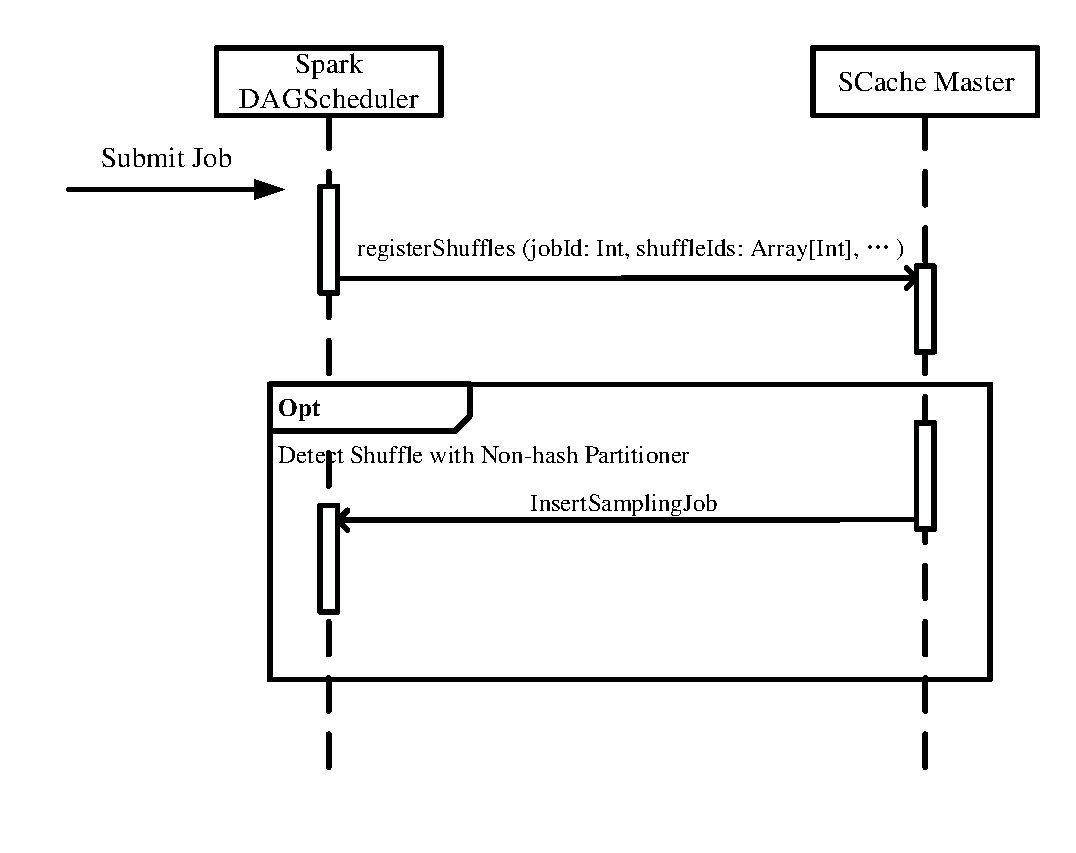
\includegraphics[width=0.8\textwidth]{shuffleregflow.pdf}
	\bicaption[fig:regshuffle]{注册shuffle时序图}{注册shuffle时序图}{Fig}{Sequence Diagram of Shuffle Registration}
\end{figure}

当一个Spark的工作启动时,首先会根据用户的代码生成一个关于RDD(Resilient Distributed Datasets)的系带关系(lineage)。
之后Spark的调度器会从最终的用户RDD递归向前寻找依赖的RDD。
在RDD之间的数据依赖中,如果存在部分依赖,也就是shuffle依赖,Spark会在此处插入一个shuffle过程,并且将之前的所有RDD合并成一个计算阶段(stage)。
递归寻找的过程会在当一个RDD的数据已经被计算或者已经到了存储系统的部分就会停止。
而这些计算阶段则最终组成了计算过程中的DAG逻辑。

对于DAG中相邻计算阶段之间的shuffle依赖,它们会被打包成一个RPC的调用提交到SCache的从属调度器上。如表\ref{tab:apis}中,一个shuffle依赖需要包含一个唯一的整数ID代表该Spark应用程序。
同时该RPC还需要包含这个shuffle依赖中每个shuffle的ID,以及它们对应的分区函数的类型,map阶段任务数和reduce阶段的任务数。
在收到注册shuffle的RPC之后,SCache的DAG附属调度器会首先检查分区函数的类型,如果不是哈希分区函数,就会通过在Spark的Driver上的守护进程在Spark执行该计算阶段前插入一段采样程序。
我们会在章节\ref{sec:sampling}和章节\ref{sec:impl}中详细阐述这个过程。

在之后的map计算阶段任务执行与shuffle数据收集过程中的时序图如图\ref{fig:putblock}所示。

\begin{figure}[!htp]
	\centering
	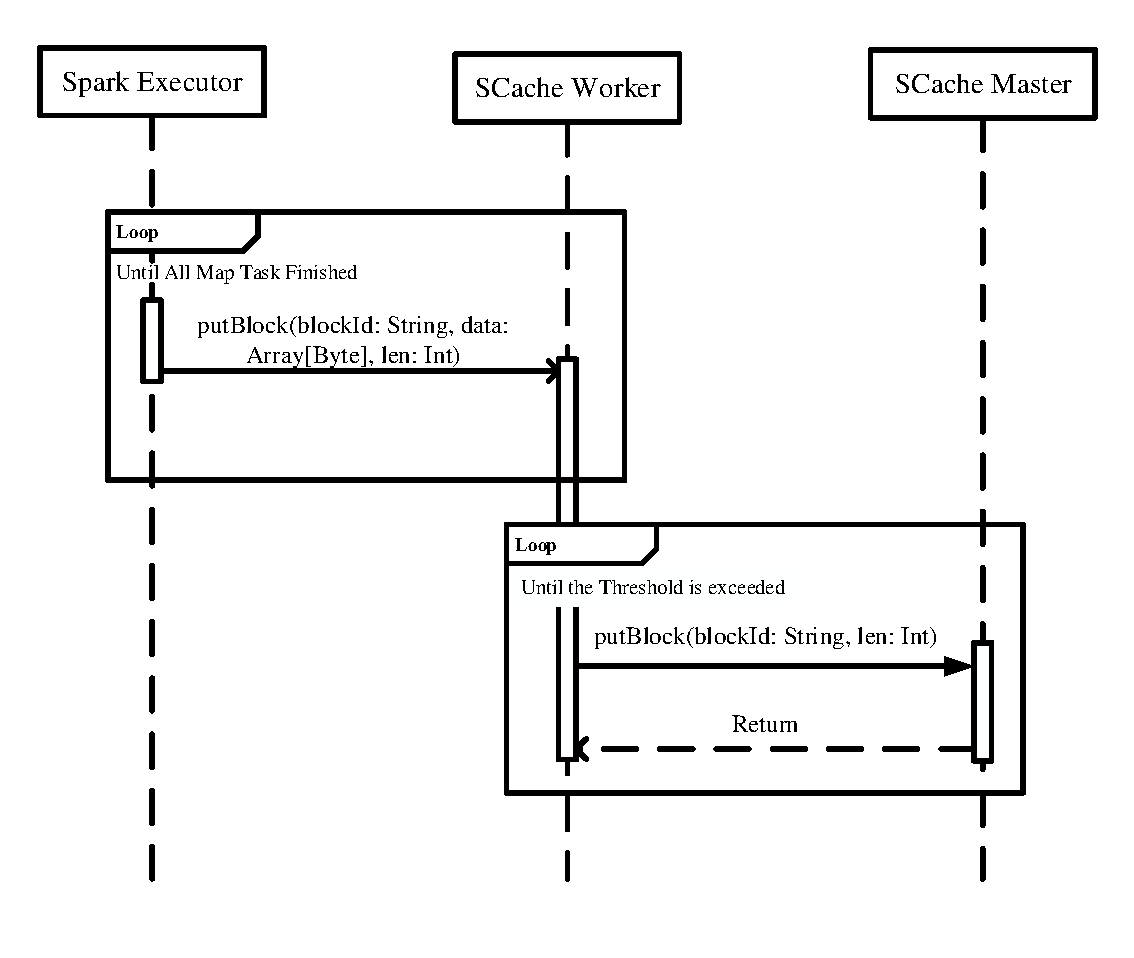
\includegraphics[width=0.8\textwidth]{putblock.pdf}
	\bicaption[fig:putblock]{Map阶段shuffle数据收集时序图}{Map阶段shuffle数据收集时序图}{Fig}{Sequence Diagram of Shuffle Data Collection in Map Stage}
\end{figure}

对于一个哈希分区函数的map任务,当计算结束之后分区函数会将计算产生的键值对通过相应的哈希函数划分成不同的数据块。
对于每一个数据块,SCache在Spark系统中的daemon程序都会根据其所在的工作ID对应的shuffle依赖ID,map任务ID,和reduce任务ID对每个数据块进行一个唯一的编号(即表格\ref{tab:apis}中的blockId)。
在此之后daemon程序会首先通过RPC的方式将这些shuffle数据块的元数据发送给SCache本地节点的工作进程。
与此同时,daemon进程也会通过Java对象的序列化的方式,将相应的数据序列化成字节码。
当接收到元数据之后,SCache的本地进程就会通过内存拷贝的形式,将序列化之后的字节码数据从Spark执行器的Java虚拟机的内存空间通过daemon程序拷贝到外部SCache的内存空间。
一旦内存拷贝结束,该map任务所占用的计算资源(slot)就会被立即释放。
通过SCache此处的内存拷贝优化,避免了原先阻塞的磁盘I/O操作,从而实现了map阶段更细粒度的硬件资源管理,提高了硬件资源的利用率和复用率。

在SCache的本地进程获取了该map任务输出的shuffle数据块之后,它会通过SCache系统内部的RPC接口通知SCache的主节点,并且在通知中附上了该map任务对于所有reduce任务产生的shuffle数据块大小(如图\ref{fig:shuffle}中的“map output”)。
每个数据块的大小可以通过内存拷贝时每个“blockId”对应的字节数组的长度来获得(即接口\ref{tab:apis}中putBlock的参数len: Int)。
当SCache的主节点收到了足够多的shuffle数据块信息之后(该threshold可以通过配置文件更改),会通过线性回归模型首先对reduce任务的输入数据分布进行预测。
之后DAG附属调度器会根据对shuffle的预测数据,调用算法\ref{mhminheap}和算法\ref{hminheap}来对reduce任务进行预调度。

\begin{figure}[!htp]
	\centering
	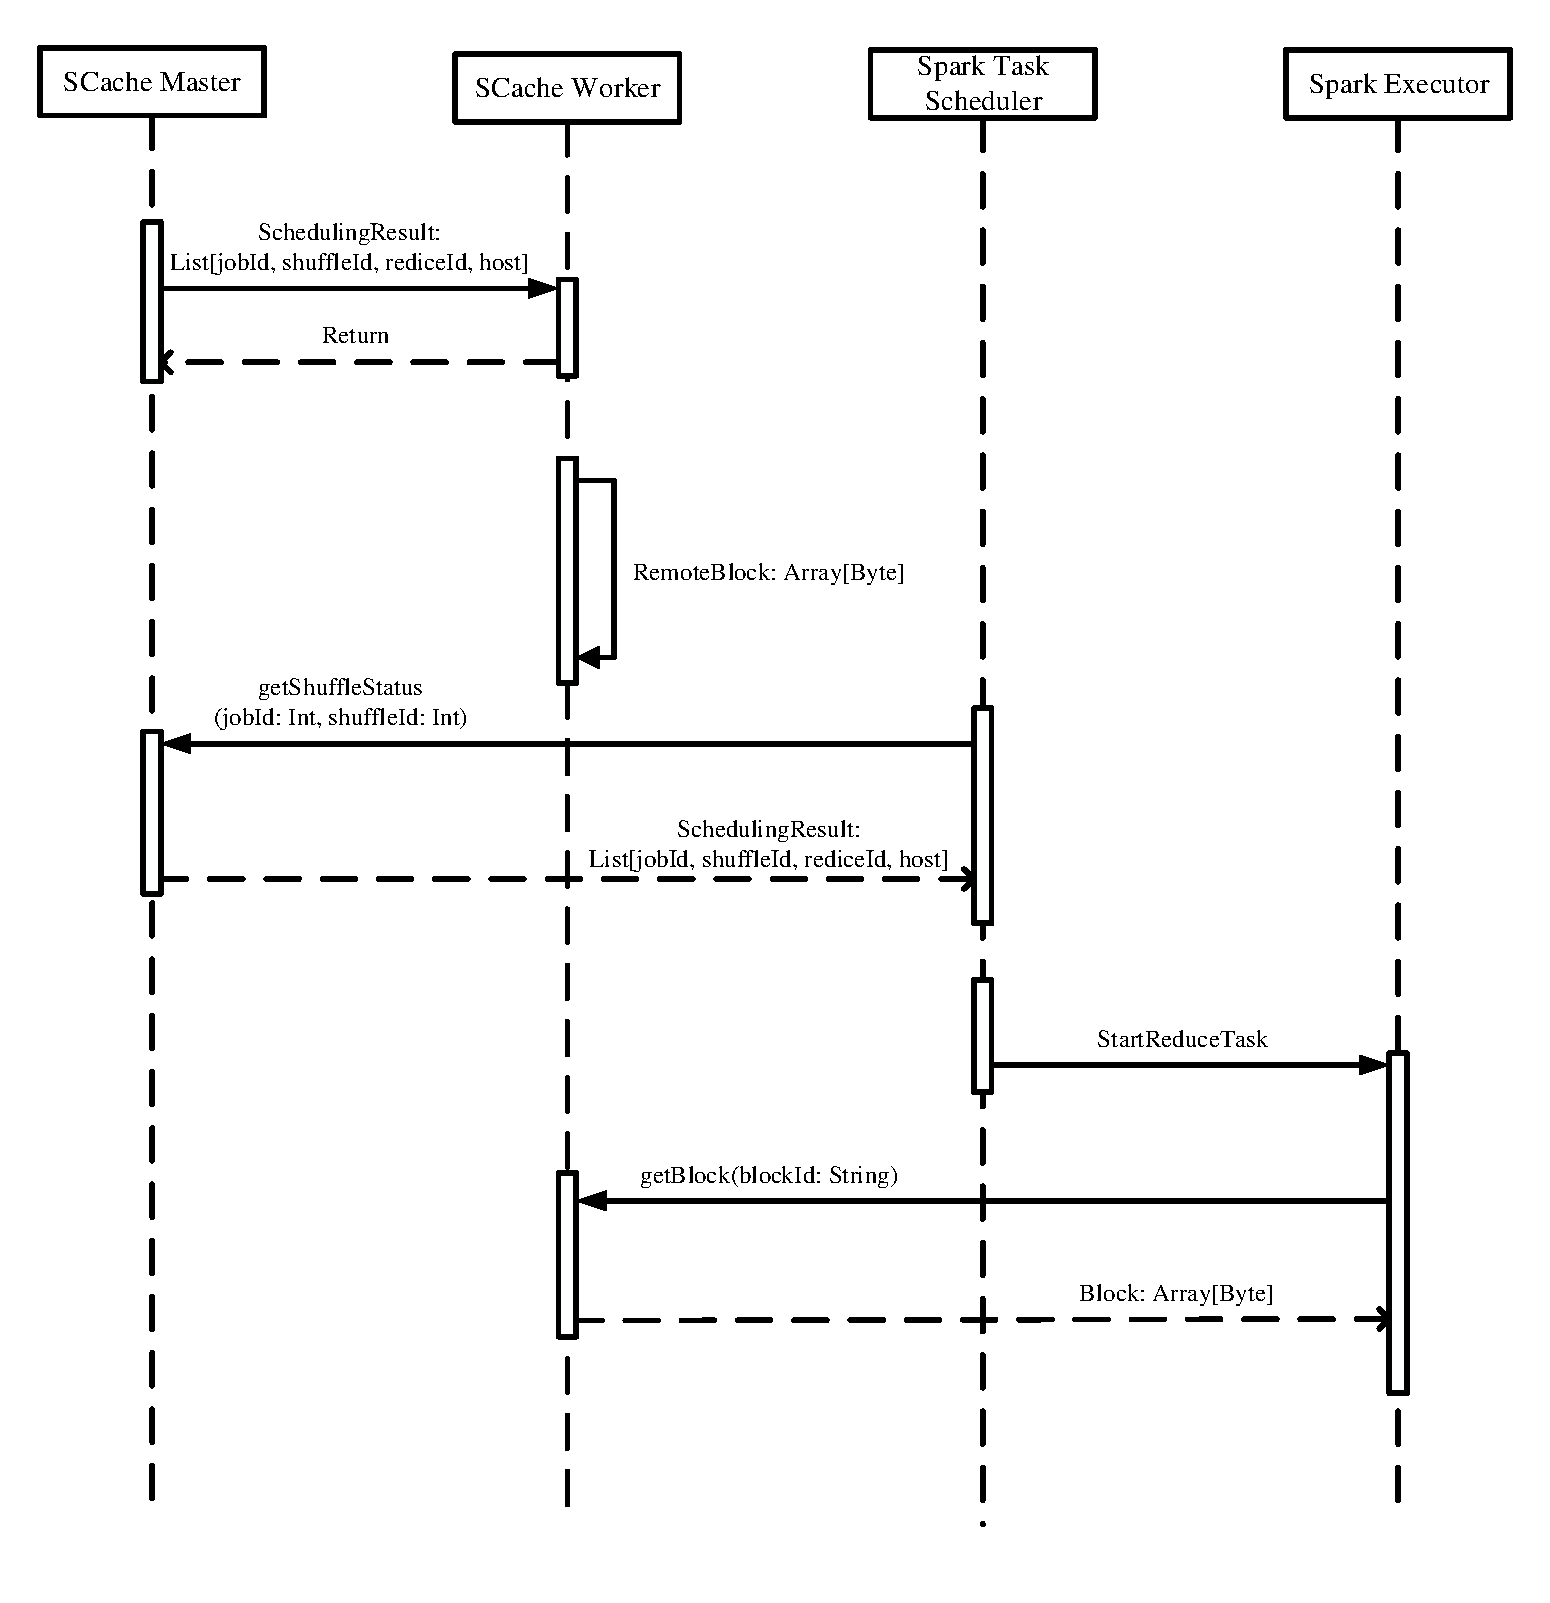
\includegraphics[width=0.8\textwidth]{preschedule.pdf}
	\bicaption[fig:preschedule]{预调度与预取工作时序图}{预调度与预取工作时序图}{Fig}{Sequence Diagram of Pre-scheduling and Pre-fetching}
\end{figure}

在SCache的中心节点完成预调度之后的流程具体如图\ref{fig:preschedule}所示。
当预调度算法运行结束之后,SCache的主节点会将reduce任务与计算节点的映射关系进行广播。
每个工作节点的SCache进程收到预调度的信息之后,会根据节点信息做出筛选,选出需要在本地执行的reduce任务。
此后本地节点会根据相应的工作ID,shuffle依赖ID,map任务ID,以及即将在本地执行的reduce任务ID组合而成的blockId,查询获取该数据块所在的节点位置,之后便开始从该远程节点预取数据。
当一个数据块被预取之后,其在节点的内存缓存就会被释放。

在reduce任务被调度的阶段,为了使Spark任务调度器遵循SCache的预调度结果,我们修改Spark的DAG调度器,通过表\ref{tab:apis}中getShuffleStatus的接口获取SCache预调度的任务 --- 节点映射关系。
在此基础上,我们将reduce任务中分配的节点修改成预调度的结果,从而使redcue任务在执行过程中获得shuffle数据预取与内存缓存的优化。

\section{水塘抽样}
\label{sec:sampling}

在上文的工作流程中,如果在注册shuffle时SCache检测到不是哈希分区函数,则SCache部署在Spark主节点上的守护进程会在使用非哈希分区函数的RDD中调用其$mapPartitionsWithIndex$\cite{sparksource}方法对每个分区的数据进行水塘采样。
如图\ref{fig:sample}所示,对于每个计算节点的本地采样程序,我们使用了经典的水塘采样算法\cite{reservoir},对每个数据分区中的输入数据进行随机采样计算并且统计经过分区函数分区后的输出shuffle数据分布。
在具体实现中,对于采样的样本数,我们将其设置为“$3 \times $数据块数目”,以此来平衡采样的精确度和采样的开销。
此处采样的样本数可以根据用户配置进行调整。
在对任务数据进行采样的同时,算法也会统计该数据分区的大小,并以此作为该任务分区采样数据的权重。
最终这些数据会在SCache主节点进行汇总,并根据公式\ref{eq:sample}来得出每个map任务对应每个
reduce任务所产生的数据块大小,之后主节点会根据reduce的任务ID进行汇总,最终得出对于下一轮reduce任务输入数据体积分布的预测。
获取预测数据之后,SCache主节点会同上文的工作流程中一致,即调用算法\ref{mhminheap}和算法\ref{hminheap}来进行任务预调度以及后续的shuffle数据预取等工作。

\begin{figure}[!htp]
	\centering
	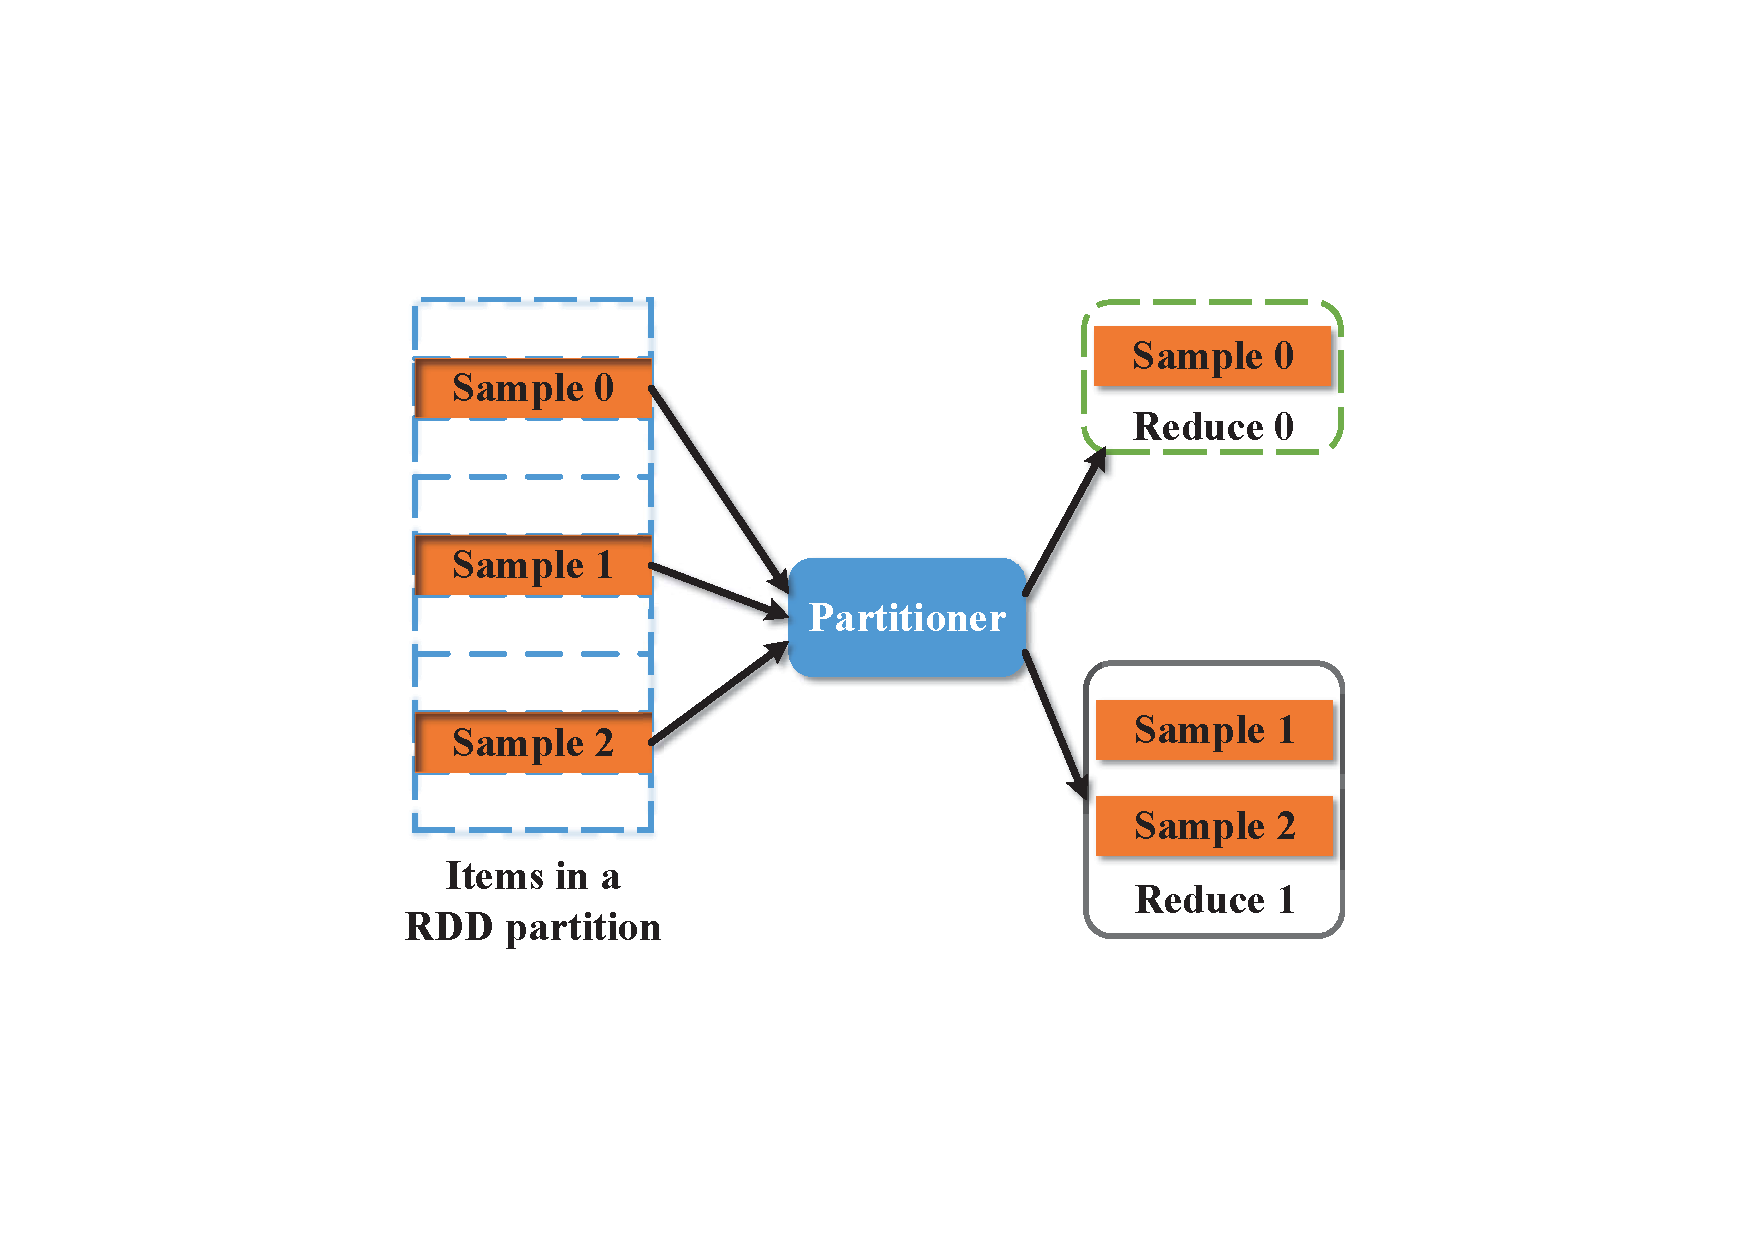
\includegraphics[width=0.6\textwidth]{../../PPoPP-2018/fig/sample.pdf}
	\bicaption[fig:sample]{对于一个任务数据分区的采样}{对于一个任务数据分区的采样}{Fig}{Reservoir Sampling of One Data Partition}
\end{figure}

\section{容错机制}

本小节将从两个角度来讨论SCache在容错性上的设计:Spark执行器或者SCache进程的崩溃造成的错误以及节点崩溃造成的节点下线的错误。

对于Spark执行器发生的错误,SCache采用了独立于Spark执行器的内存空间进行shuffle数据的存储和管理,因此即使Spark的执行器因为错误或者调度原因被Spark主节点杀死或者重启,其中所执行的任务需要的shuffle数据仍然不会遗失。

对于SCache进程的容错性,SCache采用了本地磁盘备份的机制来防止因为错误造成的shuffle数据损失。
当进行shuffle数据块预取的同时,无论该数据块是否在内存中有缓存,SCache都会在节点本地通过异步I/O的方式在本地磁盘对该数据块进行备份。
这些备份会在shuffle数据块被任务使用之后释放。
同时,SCache的工作节点会定期向主节点发送心跳信息,一旦主节点没有收到其中一个工作节点的心跳,就可以通过远程脚本控制其在本地重启。
当工作节点重启之后,主节点会向其发送当前shuffle的调度状态,工作节点则会根据本地磁盘的shuffle数据块备份状况和当前的shuffle状态来判断是否有未完成的shuffle数据块预取以及缓存任务。
而在工作节点进程失效的过程中,Spark的执行器如果有相应的reduce任务执行需要数据,则会被其中的守护进程阻塞住,直到本地工作进程完成重启。
对于SCache主节点的容错性,由于主节点的进程只服务于一个Spark的Driver程序,并且不需要调度对于跨工作的shuffle数据依赖,因此主节点采用了简单的本地磁盘备份日志的方式来备份当前对于相关shuffle的元数据记录和调度记录等信息。

为了降低系统复杂度,SCache在设计的过程中并未引入应对节点崩溃下线的容错机制。
省略这部分机制的原因主要有以下几点:
\begin{itemize}
    \item 备份机制的开销过大,与优化shuffle过程的性能目标相对立。在设计系统的过程中我们并未加入比如经典的GFS\cite{gfs}中提出的三备份机制。
    采用此类容错机制虽然能提升系统的鲁棒性,但是同时也会增加系统在执行shuffle预取与缓存过程中的开销。
    比如如果采用三备份机制,那么在shuffle数据预取阶段以及本地shuffle存储的开销都会随着备份数目的增加而倍增。
    虽然在章节\ref{subsec:size}中我们发现shuffle数据体积对较小,但是备份机制带来的额外开销无疑会给数据中心网络的性能甚至内存和硬盘的性能带来一定挑战,这也与我们的优化目标相违背。
    \item 需要备份的数据没有复用价值。对于每一个shuffle依赖中的数据,只会在DAG计算过程中被使用一次,之后便会被释放。因此对于这些数据的备份就不像一些复用性较强的存储系统甚至Spark本身的RDD来的重要。
    \item SCache与计算框架的共生性。为了提高效率,SCache采用了与DAG计算框架一一对应的共生设计,即每个计算节点既有DAG计算框架的执行器,又有SCache的工作进程。
    这种共生的模式也意味着当该节点失效时,SCache的工作进程和DAG的计算执行器会同时失效。而DAG计算框架本身又有不同的容错机制来保证任务执行。
    而此时对节点进行备份机制的设计可能不但不利于计算的快速恢复,反而会因为不同的容错策略导致SCache针对节点的容错机制变成无效操作。
    比如在Spark中,当发生数据分区因为错误而遗失时,会采取对失效的RDD分区进行并行恢复的措施。
    在此过程中原来属于一个数据分区的数据会进行再分区,从而加快恢复速度。
    那么此时针对SCache单节点的容错机制即使恢复了丢失的shuffle数据,该份数据在计算中也没有使用价值。
\end{itemize}

虽然在设计中省略了对节点下线的容错性,但是为了保证DAG计算过程在发生错误时仍然能够正确执行,SCache在此处采用了借助DAG计算框架容错性的恢复模式。
比如在上文提到的Spark恢复模式中,该失效的RDD分区会进行一个重新分区的并行计算,而在此过程中,SCache对于shuffle的优化将对这部分逻辑进行重新提交和分配。
通过借助DAG计算框架本身的容错性,SCache能保证在节点下线的恢复过程中不破坏任务的正确性,同时提供对恢复中的shuffle优化。

\section{普适性分析}
\label{sec:impl}

为了验证本研究方案的普适性,本章将详细展示在工程方面改造Spark的开销。
同时也将展示在Hadoop MapReduce上的可行性分析。
通过以上两个方面的分析和探索,最终可以证明SCache提供的优化方案可以在不需要大量改造成本的情况下即可适配目前主流的分布式DAG框架。

\subsection{Spark的实现分析}
本次实现中,我们利用Spark这个被广泛应用的分布式DAG计算平台来对SCache的优化进行适配。
在Spark上的修改主要集中在以下几个方面。

首先,我们通过netty\cite{netty}的RPC库在Spark内部实现了一个守护进程 --- \verb|ScacheDaemon|。
在\verb|ScacheDaemon|中,我们实现了表格\ref{tab:apis}中的相应接口,具体代码片段如代码\ref{code:daemon}所示。
其中变量\verb|daemon|是SCache在本地的工作进程,可以通过读取配置文件来获取具体端口,来建立连接,\verb|daemon|本身是一个netty的RPC参考(Reference)实例。
实现中的所有接口都会通过\verb|daemon|这个RPC的参考实例与本地的工作进程和SCache主节点进行数据交互。

\begin{lstlisting}[style={myScalastyle}, caption={ScacheDaemon代码片段}, label={code:daemon}]
    private[spark] class ScacheDaemon (conf: SparkConf) extends Logging {

        val scacheHome = conf.get("spark.scache.home", "~/SCache")
        val platform = "spark"  
        val daemon = new Daemon(scacheHome, platform)   
        val reduceStatus = new ConcurrentHashMap[(Int, Int), mutable.HashMap[Int, Array[String]]]() 
        private var runningJId: Int = -1    
        def setRunningJId(jid: Int): Unit = {
          //Set current runing job id
        }   
        def getRunningJId: Int = runningJId 
        def putBlock (blockId: BlockId, data: Array[Byte], rawLen: Int, compressedLen: Int): Boolean = {
          // Called by Spark Executor
          // The block data is transfered from JVM space of Spark Executor
        }   
        def getBlock(blockId: BlockId): Option[Array[Byte]] = {
          // Called by Spark Executor
          // The block data is fetched from memory of SCache to Spark Executor
        }   
        def registerShuffles(jobId: Int, shuffleIds: Array[Int], maps: Array[Int], reduces: Array[Int], partitioner: Array[String]): Unit = {
          // Called by Spark DAG Scheduler
          // Register shuffle to SCache
        }   
        def getShuffleStatus(jobId: Int, shuffleId: Int): mutable.HashMap[Int, Array[String]] = {
          // Called by Spark Task Scheduler
          // Get pre-scheduled reduce tasks
        }   
    }
\end{lstlisting}

其次,我们修改了Spark的\verb|DAGScheduler|来实现对DAG信息的获取。
具体可以参考如代码\ref{code:dagScheduler}。
在Spark的Driver节点上也存在相应的\verb|Daemon|进程。
当Spark的\verb|DAGScheduler|在从最终的RDD递归向前建立DAG的过程中(\verb|getParentStages|函数),如果发现RDD之前的依赖关系是shuffle依赖,则通过\verb|env.scacheDaemon|
获取本地已经初始化好的守护进程实例,并通过\verb|registerShuffles|接口向SCache提交该shuffle依赖的元数据。

\begin{lstlisting}[style={myScalastyle}, caption={DAGScheduler代码片段}, label={code:dagScheduler}]
    private[spark] class DAGScheduler(...) extends Logging {
      // Skip
      private def getParentStages(rdd: RDD[_], firstJobId: Int): List[Stage] = {
        val parents = new HashSet[Stage]
        val visited = new HashSet[RDD[_]]
        val waitingForVisit = new Stack[RDD[_]]
        def visit(r: RDD[_]) {
          if (!visited(r)) {
            visited += r
            val shuffles = new ArrayBuffer[ShuffleDependency[_, _, _]]
            for (dep <- r.dependencies) {
              dep match {
                case shufDep: ShuffleDependency[_, _, _] =>
                  parents += getShuffleMapStage(shufDep, firstJobId)
                  shuffles.append(shufDep)
                case _ =>
                  waitingForVisit.push(dep.rdd)
              }
            }
            if (!shuffles.isEmpty && sc.getConf.getBoolean("spark.scache.enable", false)) {
              env.scacheDaemon.registerShuffles(firstJobId, shuffles.toArray, rdd.partitions.length, rdd.partitioner.get.toString)
            }
          }
         }
        waitingForVisit.push(rdd)
        while (waitingForVisit.nonEmpty) {
          visit(waitingForVisit.pop())
        }
        parents.toList
      }
    }
\end{lstlisting}
\begin{lstlisting}[style={myScalastyle}, caption={ScacheBlockObjectWriter代码片段}, label={code:writer}]
    class ScacheBlockObjectWriter (...)extends DiskBlockObjectWriter(...) with Logging{
      override def open(): DiskBlockObjectWriter = {
        // Open a byte stream buffer
      }
      override def close(): Unit = {
        // Do memory copy and free memory
      }
      override def write(key: Any, value: Any): Unit = {
        // Write data to byte stream buffer
      }
    }
\end{lstlisting}
同时,为了使Spark的执行器在执行map任务时能够将数据发送给SCache,我们实现了一个\verb|ScacheBlockObjectWriter|用来完成map任务的shuffle数据内存拷贝。
\verb|ScacheBlockObjectWriter|实现了对Spark原来的\verb|DiskBlockObjectWriter|的继承,并且重载了其中的方法。
代码\ref{code:writer}展示了\verb|ScacheBlockObjectWriter|在继承过程中对比较重要的几个方法实现了重载。
在这里去掉了原先的磁盘写操作,取代的是对内存缓存空间的数据写入以及内存拷贝,从而优化了map计算任务的磁盘阻塞。

而在reduce阶段,我们修改了\verb|ShuffleBlockFetcherIterator|中获取shuffle数据的方法,即调用\verb|ScacheBlockTransferService|中的相应接口来从SCache获取shuffle的数据块。
虽然此处的数据访问通过内存拷贝来完成,但是为了进一步提高性能,以及预防在网络极端拥塞的情况下,最后一轮的几个map任务的输出shuffle数据仍然没有传输完成,在向SCache获取shuffle数据块的时候,
采用了多线程异步非阻塞的方式。
这种实现方式能在第一时间将已经缓存的shuffle数据块返回给Spark的reduce任务进行计算,因而能将获取shuffle数据时产生对计算的阻塞的可能性降到最低。
代码片段如代码\ref{code:reader}所示。

在reduce任务预调度方面,Spark的\verb|DAGScheduler.scala|类使其在生成reduce任务时先通过调用RDD的\verb|getPreferredLocations|方法来查询该RDD每个分区对节点的偏好。
而其中对于shuffle的传输,Spark通过\verb|ShuffledRDD.scala|这个类来具体实现,因此我们通过修改\verb|ShuffledRDD.scala|中\verb|getPreferredLocations|方法,将SCache预调度的结果通过接口\ref{tab:apis}中\verb|getShuffleStatus|返回给RDD。
具体过程可以参考代码\ref{code:preschedule}
获取预调度结果之后,Spark的\verb|TaskSchedulerImpl.scala|就会在调度reduce任务时将其分配到已经完成shuffle数据预取的节点上,从而获得SCache的优化。

\begin{lstlisting}[style={myScalastyle}, caption={ScacheBlockTransferService代码片段}, label={code:reader}]
  class ScacheBlockTransferService(daemon: ScacheDaemon) extends Logging{
    def fetchBlocks(host: String, port: Int, execId: String, blockIds: Array[String],
        listener: BlockFetchingListener): Unit = {
          // Fetch block from SCache
          // It is a multi-thread asynchronous method 
    }
  }
\end{lstlisting}
\begin{lstlisting}[style={myScalastyle}, caption={Reduce预调度代码片段}, label={code:preschedule}]
    class ShuffledRDD[...](...){
        //Skip
        override protected def getPreferredLocations(partition: Partition): Seq[String] = {
            if (SparkEnv.get.conf.getBoolean("spark.scache.enable", false)) {
              val dep = dependencies.head.asInstanceOf[ShuffleDependency[K, V, C]]
              // Ask SCache to get preferred location
              val locs = SparkEnv.get.scacheDaemon.getShuffleStatusForPartition(dep.shuffleId, partition.index)
              locs.toSeq
            } else {
              // Spark default locality mechanism
            }
        }
    }
\end{lstlisting}

在插入采样程序部分,我们利用了Spark中\verb|RangePartitioner|在决定分区边界时对RDD进行计算的过程,在其中插入了采样过程。
为了提高效率,对RDD数据的采样以及分区的计算是在Spark的Driver内部进行。
计算完成之后再将数据发送给SCache,具体逻辑如代码\ref{code:sample}所示。
其中返回的\verb|distribution|将会作为采样的分布通过接口\ref{tab:apis}中的\verb|sampling|发送给SCache。
以上四个部分是在Spark适配过程中做出的主要改动,其代码量大约在1000行左右,相较于Spark本身几十万行的代码量,可以说这个改动是非常的小。

\begin{lstlisting}[style={myScalastyle}, caption={水塘采样代码片段}, label={code:sample}]
    def determineBounds[K : Ordering : ClassTag](
      candidates: ArrayBuffer[(K, Float, Int)], partitions: Int,
      depPartitionNum: Int): (Array[K], Array[Array[Int]]) = {
        // Skip
        val ordered = candidates.sortBy(_._1)
        val distribution = Array.fill[Int](depPartitionNum)(0)
          .map(x => new Array[Float](partitions))
        var i = 0
        var j = 0
        var previousBound = Option.empty[K]
        while ((i < numCandidates) && (j < partitions - 1)) {
          val (key, weight, index) = ordered(i)
          cumWeight += weight
          distribution(index)(j) += weight
          if (cumWeight >= target) {
            // Skip duplicate values.
            if (previousBound.isEmpty || ordering.gt(key, previousBound.get)) {
              bounds += key
              target += step
              j += 1
              previousBound = Some(key)
            }
          }
          i += 1
        }
        while (i < numCandidates) {
          // calculate the distribution of last partition
          val (key, weight, index) = ordered(i)
          distribution(index)(j) += weight
          i += 1
        }
        (bounds.toArray, distribution)
    }
\end{lstlisting}

\subsection{Hadoop MapReduce的可行性分析}

受限于时间,本研究并没有对Hadoop MapReduce进行SCache的适配改造。
但是为了验证SCache对shuffle的优化的普适性,本研究仍对Hadoop MapReduce的适配可行性进行了分析研究。

首先,我们对Hadoop MapReduce的计算过程中存在的shuffle特点进行分析。
虽然在表达DAG的过程中Hadoop MapReduce与Spark存在较大差异,但是在每个map和reduce的计算阶段之间都会存在一个shuffle的过程却十分接近。
在执行map任务时,Hadoop MapReduce中的\verb|MapTask.java|类
会将map任务计算产生的shuffle结果通过\verb|MapOutputCollector.java|接口写入到本地磁盘进行保存。
当reduce任务数目不为0时,即该map阶段不是分布式应用的最后一次计算阶段时,map任务会调用\verb|NewOutputCollector.java|来写入该阶段的输出键值对。
在具体执行过程中,其通过实例化一个\verb|collector|来进行写操作,而该\verb|collector|就是一个\verb|MapOutputCollector.java|的具体实例。
具体代码参考代码片段\ref{code:hadoopmap}

\begin{lstlisting}[language={Java}, caption={Hadoop MapReduce中Map阶段的shuffle写代码片段}, label={code:hadoopmap}]
    private <...>
    void runNewMapper(...) throws ... {
        // Skip
        // get an output object
        if (job.getNumReduceTasks() == 0) {
          output = 
            new NewDirectOutputCollector(taskContext, job, umbilical, reporter);
        } else {
          output = new NewOutputCollector(taskContext, job, umbilical, reporter);
        }
        // Skip    
        try {
          long startTime = System.currentTimeMillis();
          input.initialize(split, mapperContext);
          mapper.run(mapperContext);
          mapPhase.complete();
          setPhase(TaskStatus.Phase.SORT);
          statusUpdate(umbilical);
          input.close();
          input = null;
          output.close(mapperContext);
          output = null;
        } finally {
          closeQuietly(input);
          closeQuietly(output, mapperContext);
        }
    }

    NewOutputCollector(...) throws ... {
        @Override
        public void write(K key, V value) throws ... {
          collector.collect(key, value,
                            partitioner.getPartition(key, value, partitions));
        }
        @Override
        public void close(TaskAttemptContext context) throws ... {
          try {
            collector.flush();
          } catch (ClassNotFoundException cnf) {
            throw new IOException("can't find class ", cnf);
          }
          collector.close();
        }
    }
\end{lstlisting}

在reduce阶段,每个reduce任务由类\verb|ReduceTask.java|来执行。
具体来说,每个reduce任务会通过\verb|ShuffleConsumerPlugin|的接口来实现第一阶段的远程shuffle数据拷贝过程。
在目前的MapReduce中,该接口由类\verb|Shuffle<K, V>|实现了一个多线程的异步远程shuffle数据读取。
具体可以参考代码片段\ref{code:hadoopreduce}。

\begin{lstlisting}[language={Java}, caption={Hadoop MapReduce中Reduce阶段的shuffle读代码片段}, label={code:hadoopreduce}]
    public class ReduceTask extends Task {
        public void run(...) throws ... {
          // Skip
          ShuffleConsumerPlugin.Context shuffleContext = new ShuffleConsumerPlugin.Context(...);
          shuffleConsumerPlugin.init(shuffleContext);
          // fetch the remote shuffle blocks simultaneously
          rIter = shuffleConsumerPlugin.run();
        }
    }

    public class Shuffle<K, V> implements ShuffleConsumerPlugin<K, V>, ExceptionReporter {
        // Skip
        @Override
        public RawKeyValueIterator run() throws IOException, InterruptedException {
          //Skip
          if (isLocal) {
            fetchers[0] = new LocalFetcher<K, V>(jobConf, reduceId, scheduler,
            merger, reporter, metrics, this, reduceTask.getShuffleSecret(),
            localMapFiles);
            fetchers[0].start();
          } else {
            for (int i=0; i < numFetchers; ++i) {
              fetchers[i] = new Fetcher<K,V>(...);
              fetchers[i].start();
            }
          }
        }
    }
\end{lstlisting}

而对于任务的调度,在Hadoop MapReduce中,主要由一系列状态机的转移和Yarn\cite{yarn}的资源调度机制协同完成。
具体来讲,在一个MapReduce任务被提交之后,经过一系列的状态转移,最终会由\verb|JobImpl|类来完成map和reduce阶段的具体任务生成以及提交。
而由于MapReduce的计算DAG相较于Spark十分简单,即在一个任务只有Map和Reduce两个过程,所以对于shuffle的相关元数据便可以在此处获得。
具体关于shuffle两端map和reduce任务的生成,可以参考代码\ref{code:hadoopshuffle}。

对于reduce阶段的任务预调度,在MapReduce中都是通过\verb|RMContainerAllocator.java|的类来实现的。
当其收到对reduce任务的调度的请求时,\verb|RMContainerAllocator.java|会根据从Yarn的ResourceManager那里获取的可用容器数(Container)进行分配。
具体可以参考代码片段\ref{code:hadoopschedule}

综上所述,我们给出了以下对Hadoop MapReduce的SCache适配的改造方案。
\begin{enumerate}
    \item Shuffle元数据获取:在\verb|JobImpl|类中发生任务提交而产生的状态转换函数执行过程中,可以获取shuffle两端对应的map任务个数,reduce任务个数等信息。
    此时,便可以将这些数据通过接口\ref{tab:apis}中的\verb|registerShuffles|进行提交。
    \item Map任务shuffle数据的解耦:可以通过重新实现一个对接口\verb|MapOutputCollector|的实现类来获取shuffle数据,并且通过内存拷贝传递给SCache。
    \item Reduce任务shuffle数据的解耦:可以通过重新实现一个接口\verb|ShuffleConsumerPlugin|的实现类来从SCache的内存缓存获取shuffle的数据。
    \item Reduce任务的预调度:需要将SCache的预调度结果通过接口在\verb|RMContainerAllocator.java|调度任务前对预调度结果进行获取,然后在其调用\verb|assignToReduce|函数时遵循预调度的结果即可。
    \item 采样任务的实现:在\verb|JobImpl|类中生成具体任务的时候,可以通过配置信息来获取分区函数的信息。
    如果发现是一个非哈希的分区函数,则在创建map任务的同时创建每个任务对应的采样任务对其进行数据采样。
\end{enumerate}

\begin{lstlisting}[language={Java}, caption={Hadoop MapReduce中shuffle元数据生成代码片段}, label={code:hadoopshuffle}]
    public class JobImpl implements org.apache.hadoop.mapreduce.v2.app.job.Job, EventHandler<JobEvent> {
        // Skip
        @Override
        public JobStateInternal transition(JobImpl job, JobEvent event) {
          // Skip
          createMapTasks(job, inputLength, taskSplitMetaInfo);
          createReduceTasks(job);
        }
    }
\end{lstlisting}

\begin{lstlisting}[language={Java}, caption={Hadoop MapReduce中reduce任务调度代码片段}, label={code:hadoopschedule}]
    public class RMContainerAllocator extends RMContainerRequestor implements ContainerAllocator {
        private ContainerRequest assignToReduce(Container allocated) {
          ContainerRequest assigned = null;
          //try to assign to reduces if present
          if (assigned == null && reduces.size() > 0 && canAssignReduces()) {
            TaskAttemptId tId = reduces.keySet().iterator().next();
            assigned = reduces.remove(tId);
            LOG.info("Assigned to reduce");
          }
          return assigned;
        }
    }
\end{lstlisting}

以上两个小节通过对目前最流行的Spark和Hadoop MapReduce这两个典型的分布式DAG计算框架应用SCache优化的可行性做出了具体的分析。
通过展现Spark上的具体实现技术,可以看到应用SCache的优化对于原有框架本身并不需要做出巨大的修改。
同时,通过对Hadoop MapReduce的任务执行框架任务调度流程,shuffle过程的分析,我们发现对于SCache提供的优化策略在Hadoop MapReduce上也能非常方便的适配。
因此我们认为SCache提供的优化方案对于目前主流的分布式DAG计算框架具有较好的普适性。
能够通过对现有框架较少的改动而实现适配与shuffle的优化。
\section{Evaluation}\label{evaluation}
\begin{figure}
	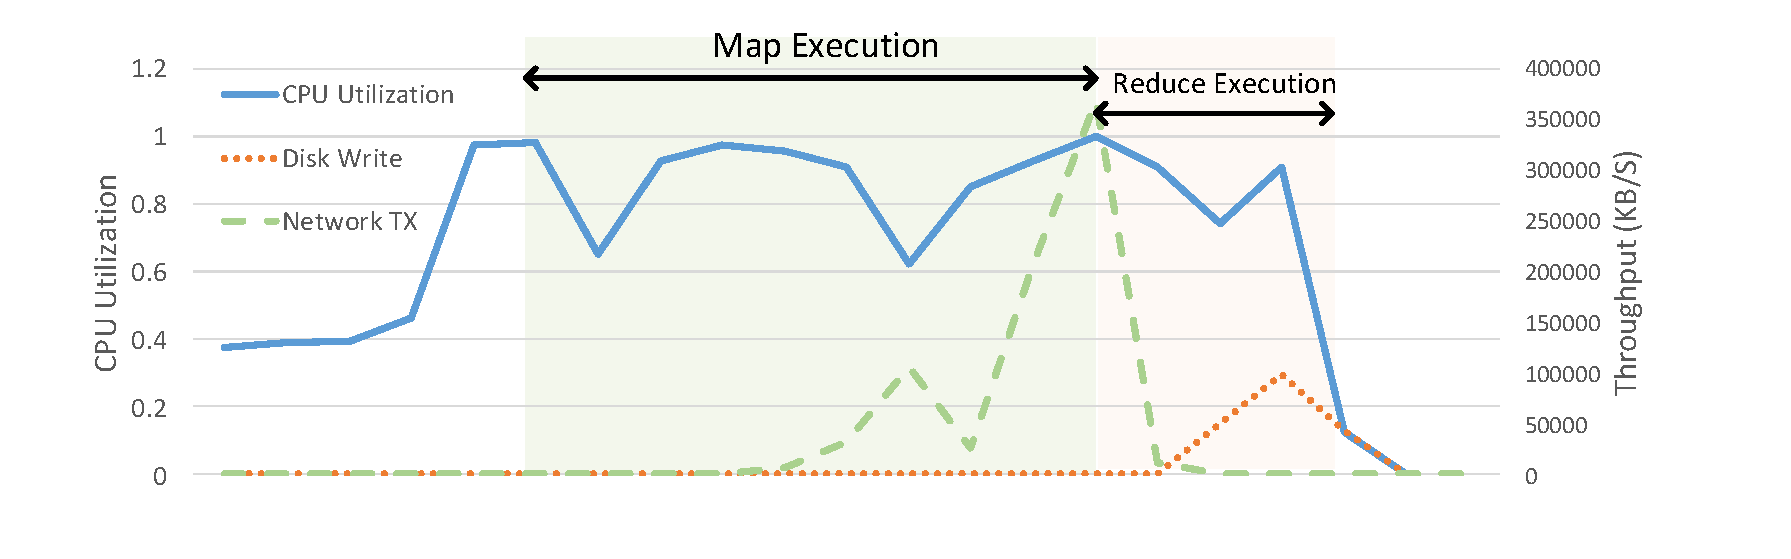
\includegraphics[width=\linewidth]{fig/scache_util}
	\caption{CPU utilization and I/O throughput of a node during a Spark single shuffle application With SCache}
	\label{fig:scache_util}
\end{figure}
In this section, we present the evaluation of SCache with comprehensive workloads and benchmarks. First we run a simple DAG job with single shuffle to analysis hardware utilization and impact of shuffle optimization from the scope of a task to a job. 
Then we use a recognized shuffle intensive benchmark --- Terasort \cite{spark-tera} to evaluate SCache with different data partition schemes.
In order to prove the performance gain of SCache with a real production workload, we also evaluate TPC-DS \cite{sparktpcds} and present the overall performance improvement.
At last, we measure the overhead of weighted reservoir sampling. 
Briefly, SCache can decrease ~$89\%$ time of Spark shuffle. SCache can also achieves a ~$75\%$ and ~$50\%$ improvement of reduce stage completion time respectively in simple DAG application and Terasort without introducing extra network traffic. More impressively, the overall completion time of TPC-DS can be improved ~$40\%$ on average by applying optimization from SCache.
% Because a complex Spark application consists of multiple stages. The completion time of each stage varies under different input data, configurations and different number of stages. This uncertainty leads to the dilemma that dramatic fluctuation occurs in overall performance comparison. To present a straightforward illustration, we limit the scope of most evaluations in a single stage.

\subsection{Setup}\label{stepup}
We implement a Spark demon to enable shuffle optimization as a representative.
We run our experiments on a 50 m4.xlarge nodes cluster on Amazon EC2 \cite{aws}. Each node has 16GB memory and 4 CPUs. The network bandwidth is not specifically provided by Amazon. Our evaluations reveal the bandwidth is about 300 Mbps (see Figure \ref{fig:util}).

\subsection{Simple DAG Analysis}
\subsubsection{Hardware Utilization}
We first run the same single shuffle test (GroupByTest from Spark example \cite{sparksource}) as mentioned in Figure \ref{fig:util}. As shown in Figure \ref{fig:scache_util}, the hardware utilization is captured from one node during the job. Note that since the completion time of whole job is about $50\%$ less than Spark without SCache, the duration of Figure \ref{fig:scache_util} is cut in half as well. An overlap between CPU, disk and network can be easily observed in Figure \ref{fig:scache_util}. That is, the I/O operations will never cut off the computing process with the fine-grained resource allocation. By running Spark with SCache, the overall CPU utilization of the cluster stays in a high level. The decoupling of shuffle write from map tasks frees the CPU earlier and leads to a faster map task computation. The shuffle pre-fetch starting in the early stage of map phase shift the network transfer completion time, so that the computation of reduce can start immediately after scheduled. The combination is the main performance gain we achieved on the scope of hardware utilization by SCache.

\begin{figure}
	%\vspace*{-0.01cm}
	\begin{subfigure}{\linewidth}
		\centering
		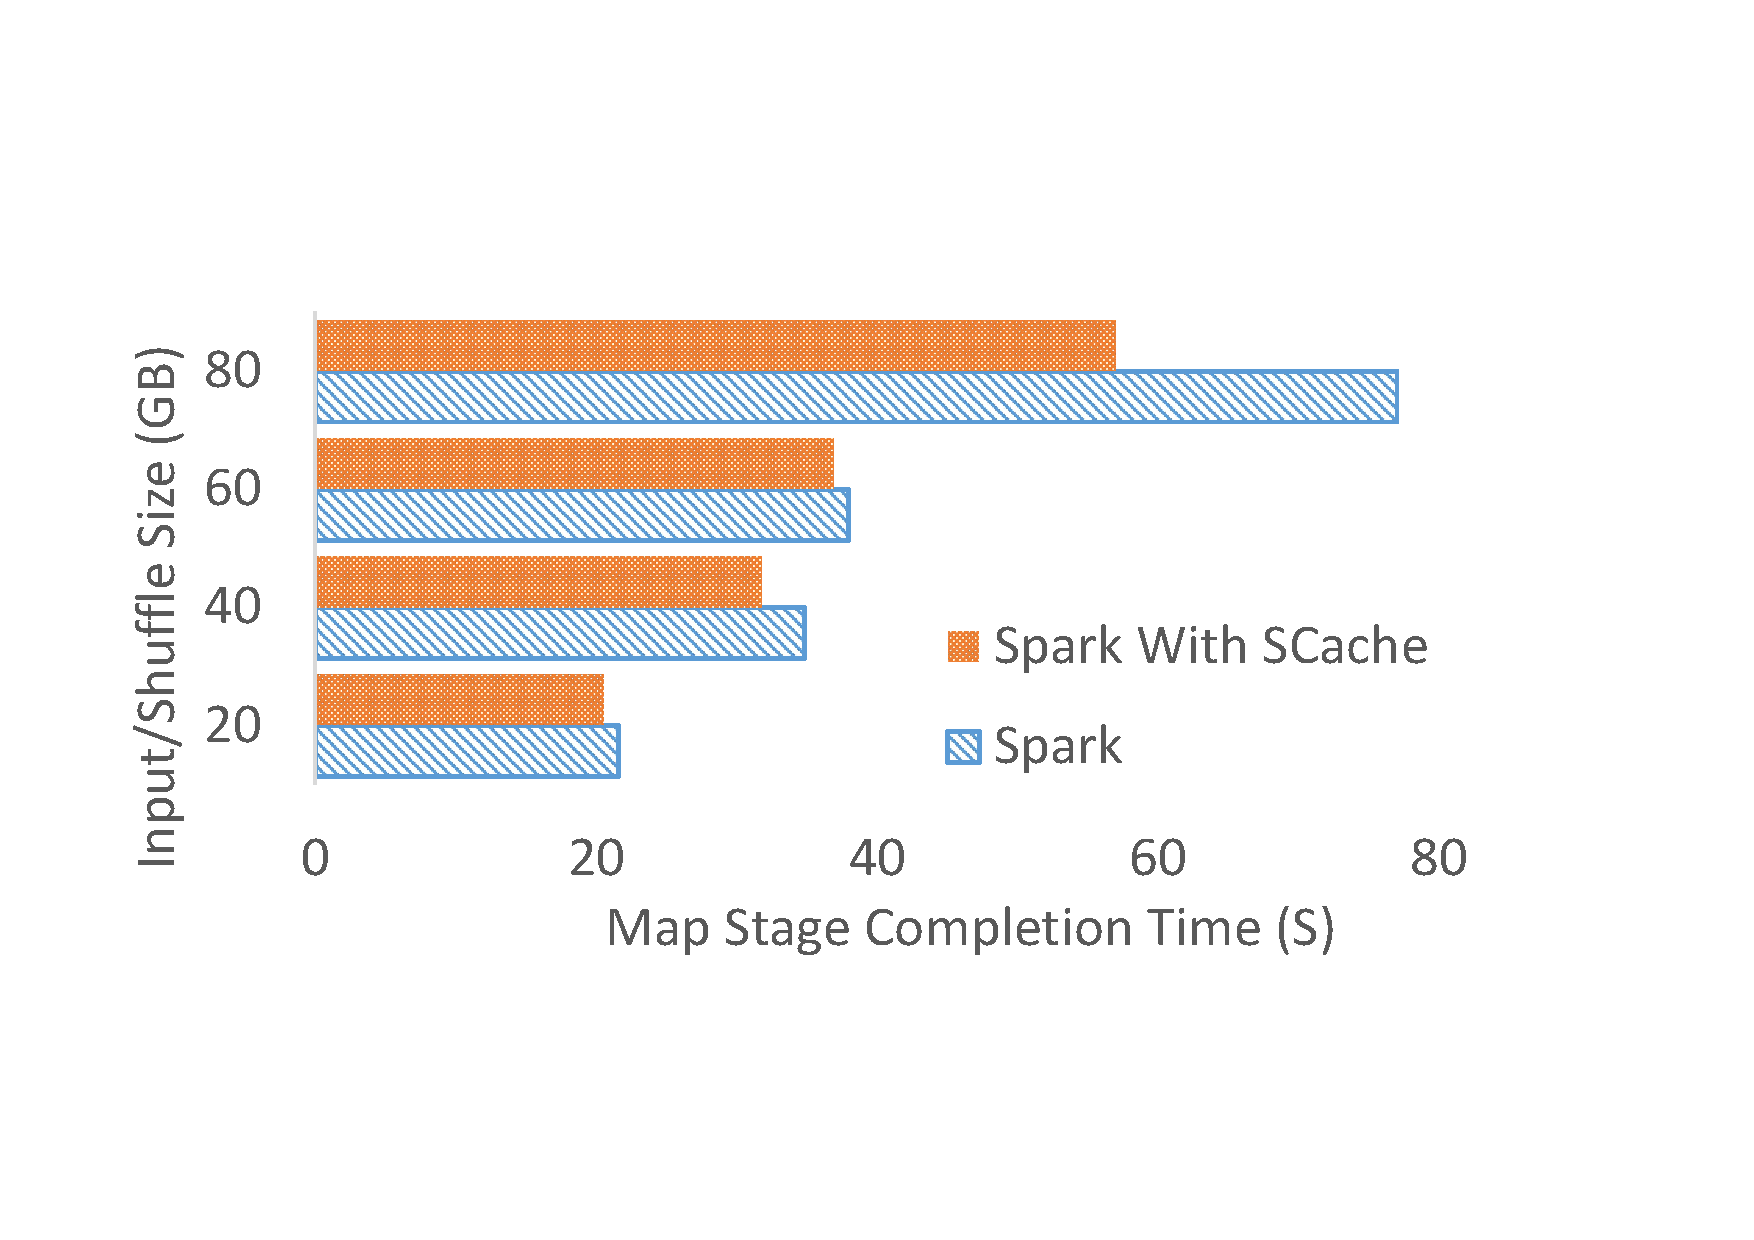
\includegraphics[width=0.9\linewidth]{fig/groupbymapstage}
		\caption{Map Stage Completion Time Comparison}
		\label{fig:mapstage}
	\end{subfigure}
	\begin{subfigure}{\linewidth}
		\centering
		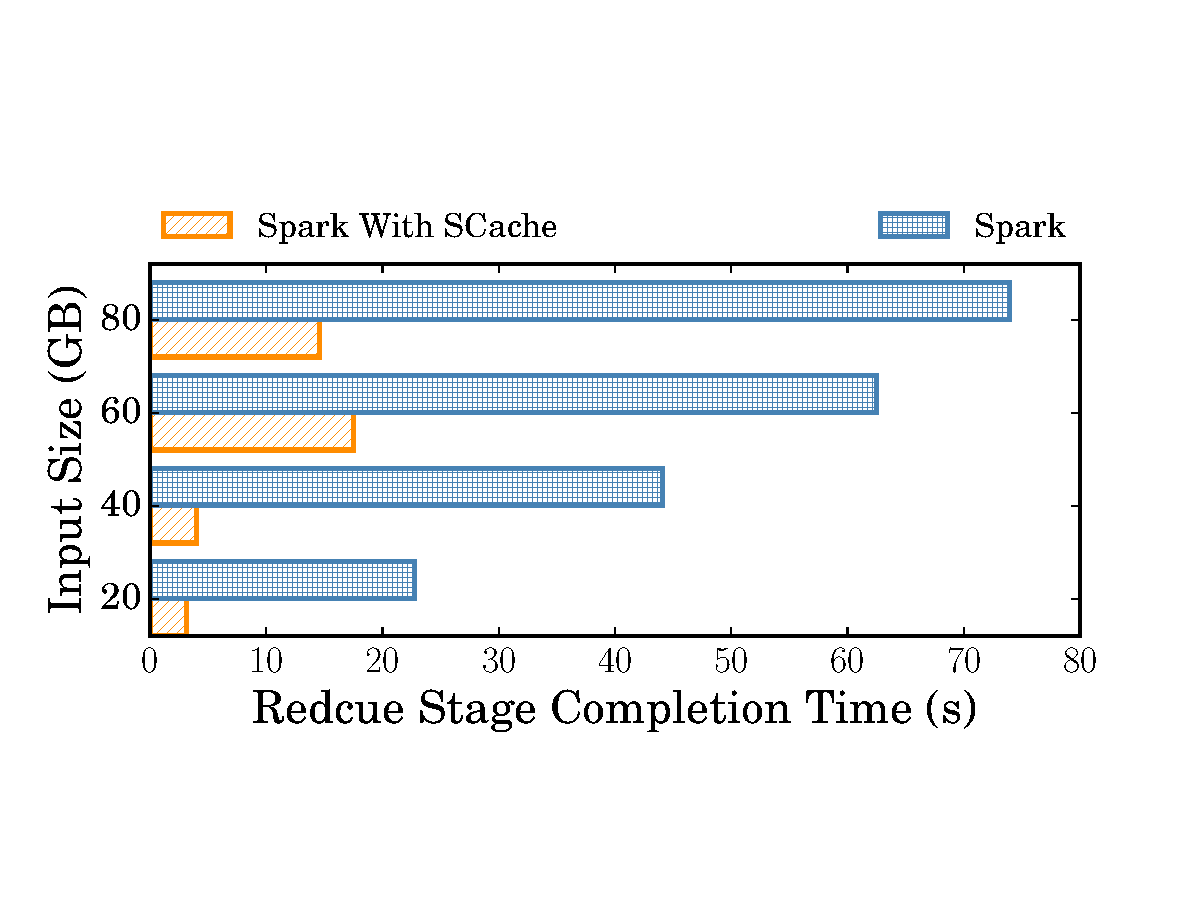
\includegraphics[width=0.9\linewidth]{fig/groupbyreducestage}
		\caption{Reduce Stage Completion Time Comparison}
		\label{fig:reducestage}
	\end{subfigure}
	\caption{Stage Completion Time of Single Shuffle Test}
	\label{fig:singleshuffle}
\end{figure}

\begin{figure}
	\begin{subfigure}{\linewidth}
		\centering
		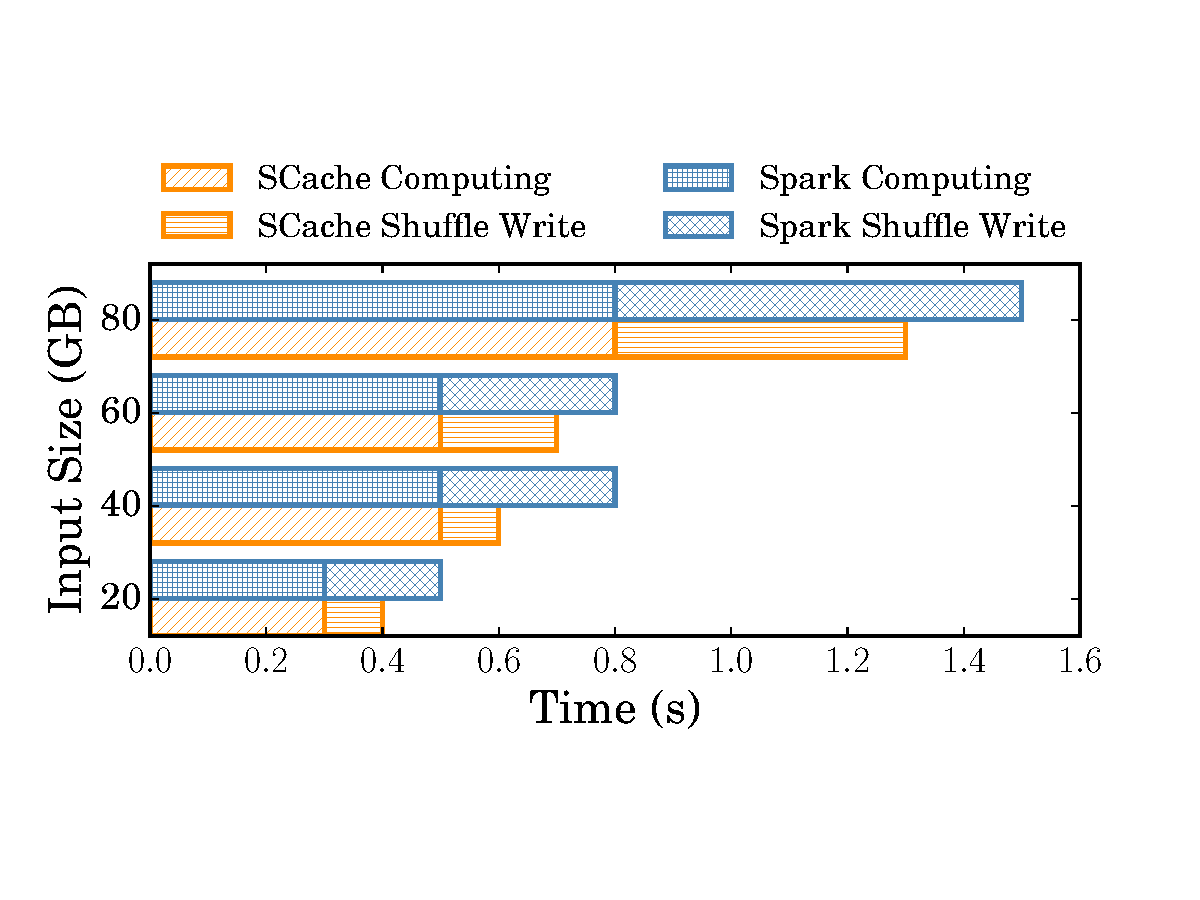
\includegraphics[width=0.9\linewidth]{fig/groupbymaptask}
		\caption{Median Task Details in Map Stages}
		\label{fig:maptask}
	\end{subfigure}
	\begin{subfigure}{\linewidth}
		\centering
		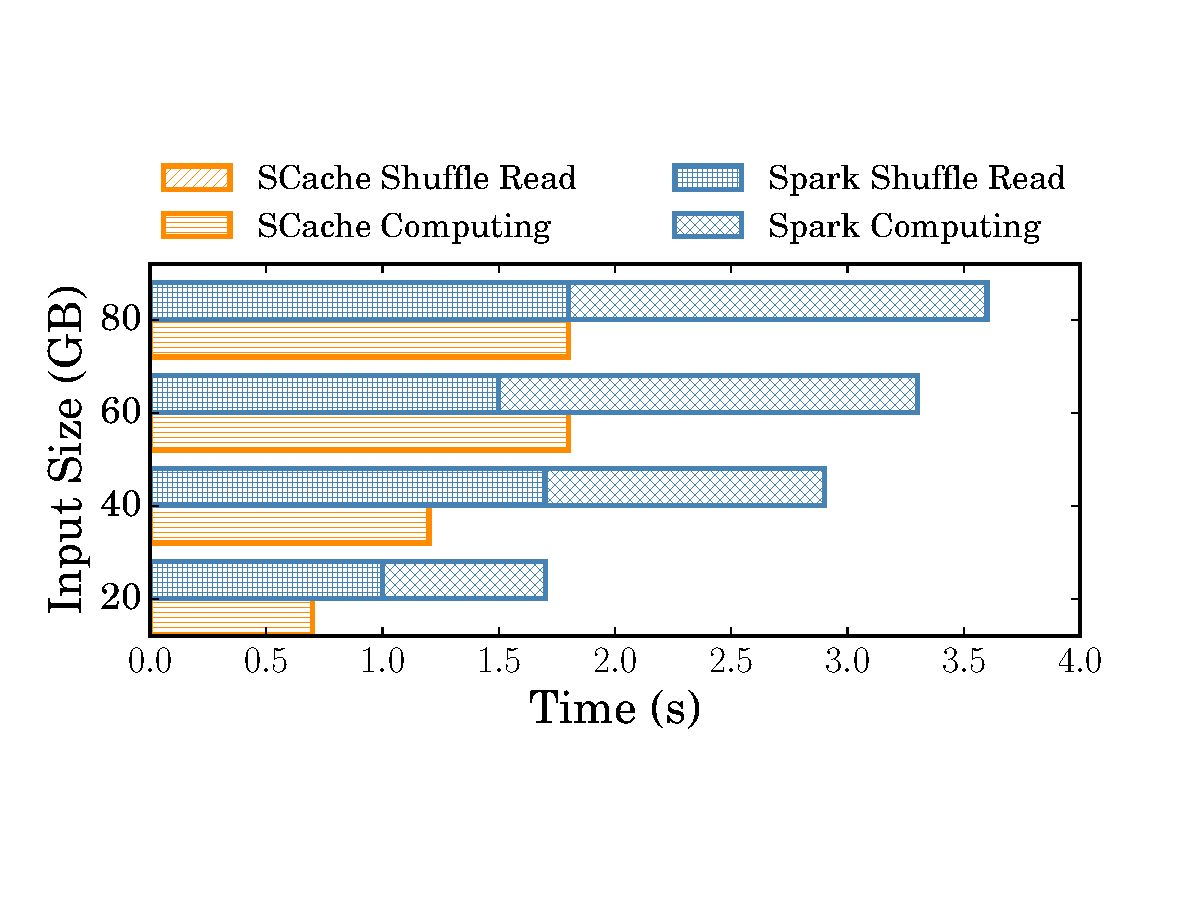
\includegraphics[width=0.9\linewidth]{fig/groupbyreducetask}
		\caption{Median Task Details in Reduce Stages}
		\label{fig:reducetask}
	\end{subfigure}
	\caption{Median Task Completion Time of Single Shuffle Test}
	\label{fig:singleshuffletask}
\end{figure}

The performance is evaluated with different input sizes in the cluster. For each stage, we run 5 rounds of tasks. The stage completion time is presented separately in Figure \ref{fig:mapstage} and Figure \ref{fig:reducestage}. By running spark with SCache, the completion time of map stage can be reduced $10\%$ on average. For reduce stage, instead, SCache achieves a ~$75\%$ performance gain in the completion time of the reduce stage.

A detail analysis into the nutshell of varied overall performance gain on different stages is presented with Figure \ref{fig:singleshuffletask}. For each stage, we pick the median task. About 40\% of shuffle write time can be eliminated by SCache (Figure \ref{fig:maptask}) in a map task. Because the serialization of data is CPU intensive \cite{makingsense} and it is inevitable while moving data out of Java heap memory, SCache can not eliminate the whole phase of shuffle write. This results in a less performance gain in the map stage.
On the reduce side, the network transfer introduces a significantly latency in shuffle read for a single task (Figure \ref{fig:reducetask}). By doing shuffle data pre-fetch for the reduce tasks in Figure \ref{fig:reducetask}, the shuffle read time decreases ~$100\%$, which means shuffle data pre-fetch almost hide all the explicit network transfer in the reduce stage. In overall, SCache can help Spark decreases by ~$89\%$ time in the whole shuffle process. In addition, heuristic reduce tasks scheduling achieves better load balance in cluster than the Spark default FIFO scheduling which may randomly assign two heavy tasks on a single node. So that we can have a significant performance gain in the completion time of the reduce stage.
% \begin{figure*}
% 	\begin{minipage}{\textwidth}
% 		\begin{figure}[H]
% 			\begin{subfigure}{0.5\textwidth}
% 				\centering
% 				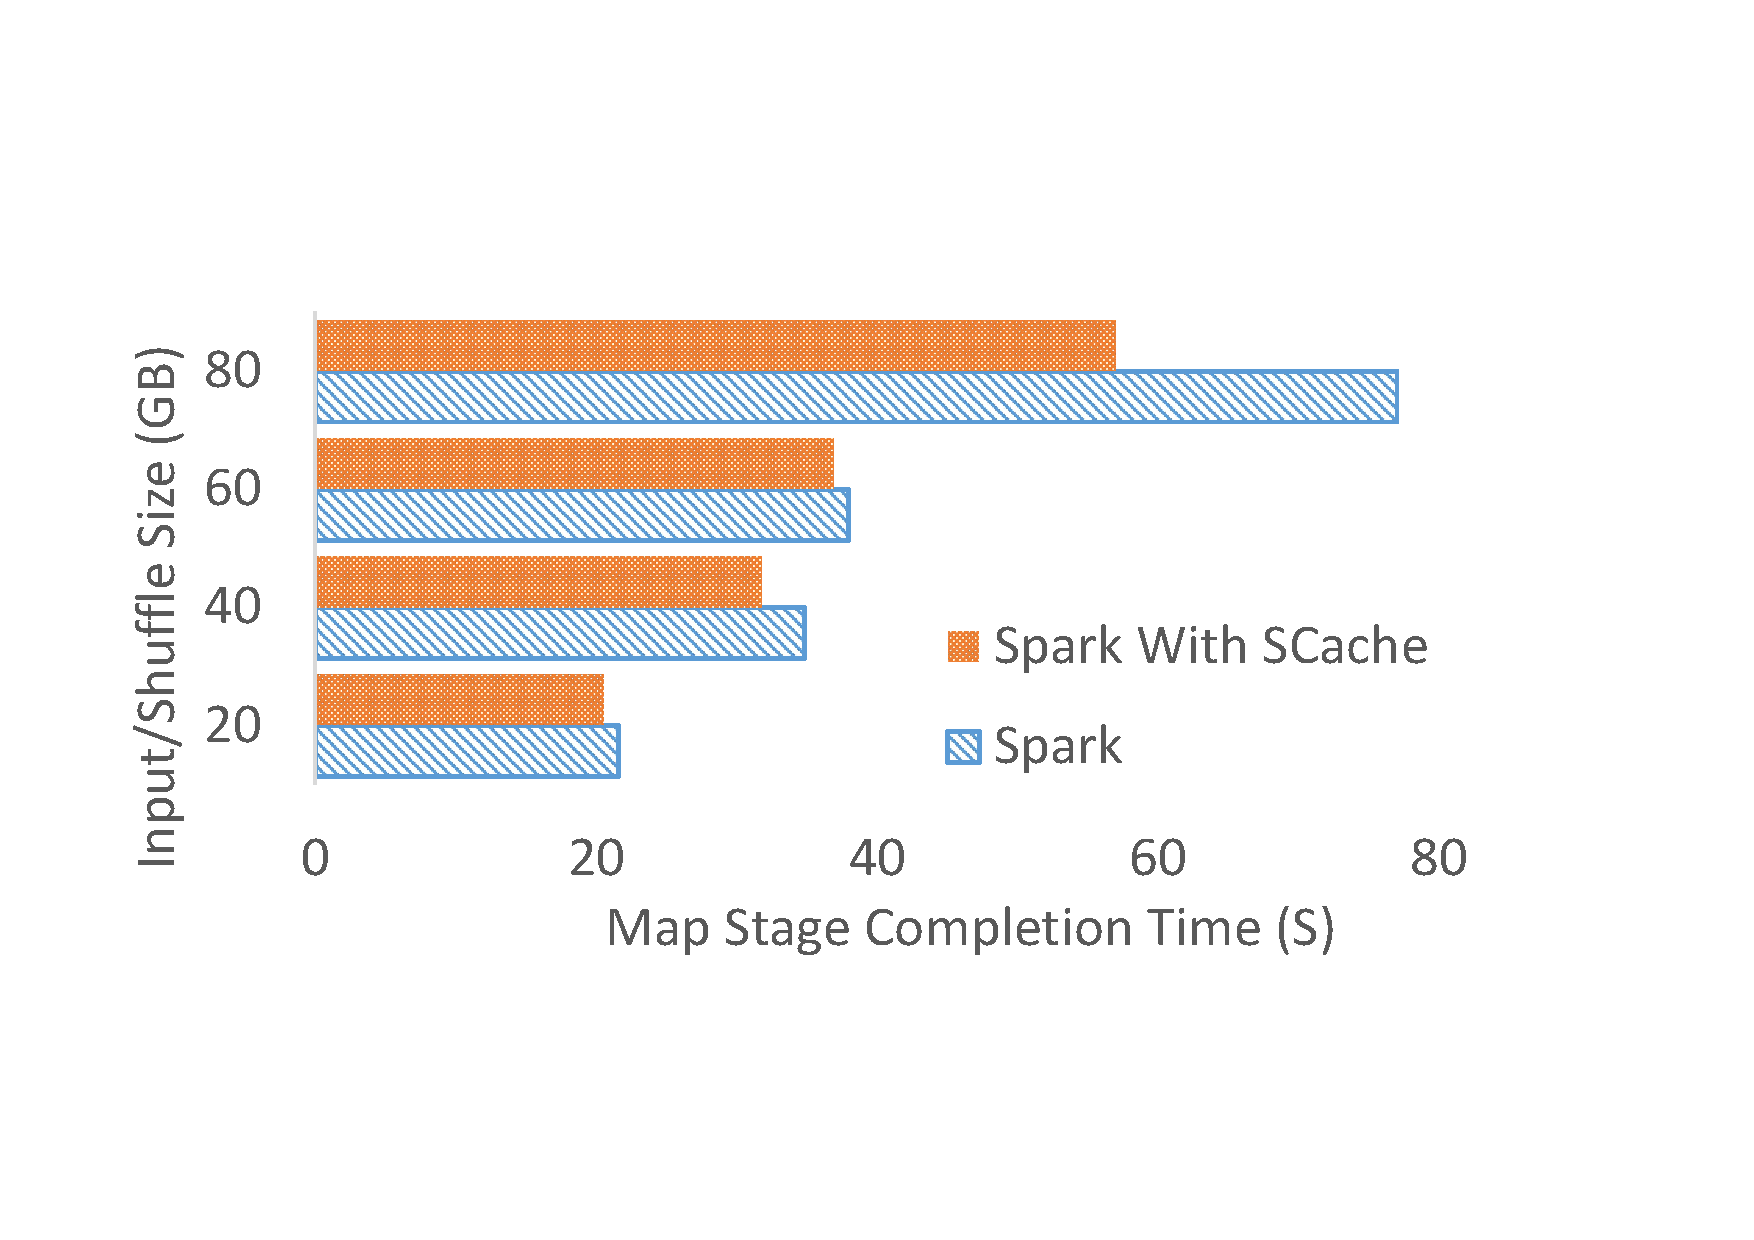
\includegraphics[width=0.8\linewidth]{fig/groupbymapstage}
% 				\caption{Map Stage Completion Time Comparsion}
% 				\label{fig:mapstage}
% 			\end{subfigure}
% 			\begin{subfigure}{0.5\textwidth}
% 				\centering
% 				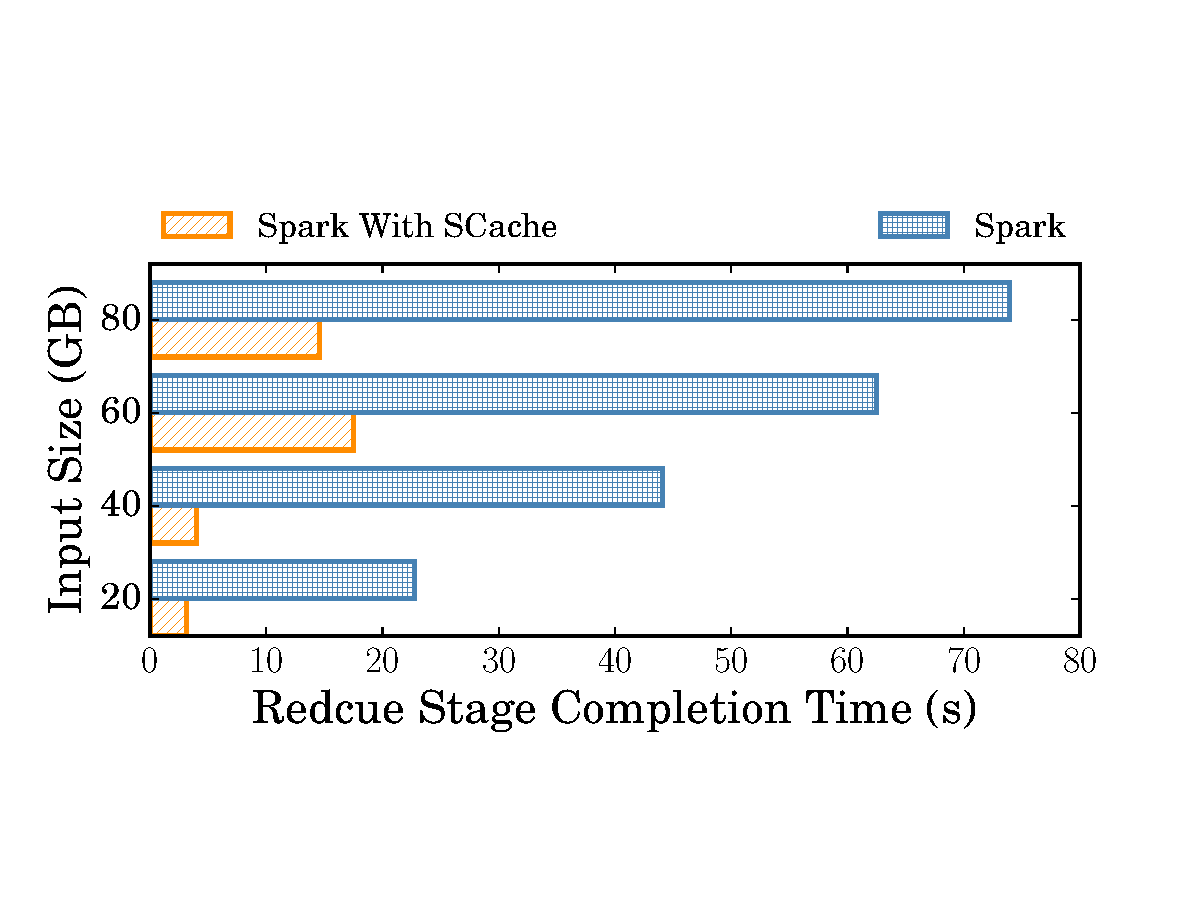
\includegraphics[width=0.8\linewidth]{fig/groupbyreducestage}
% 				\caption{Reduce Stage Completion Time Comparsion}
% 				\label{fig:reducestage}
% 			\end{subfigure}
% 			\caption{Stage Completion Time Comparsion of Single Shuffle Test}
% 			\label{fig:singleshuffle}
% 		\end{figure}
% 	\end{minipage}
% 	\begin{minipage}{\textwidth}
% 		\begin{figure}[H]
% 			\begin{subfigure}{0.5\textwidth}
% 				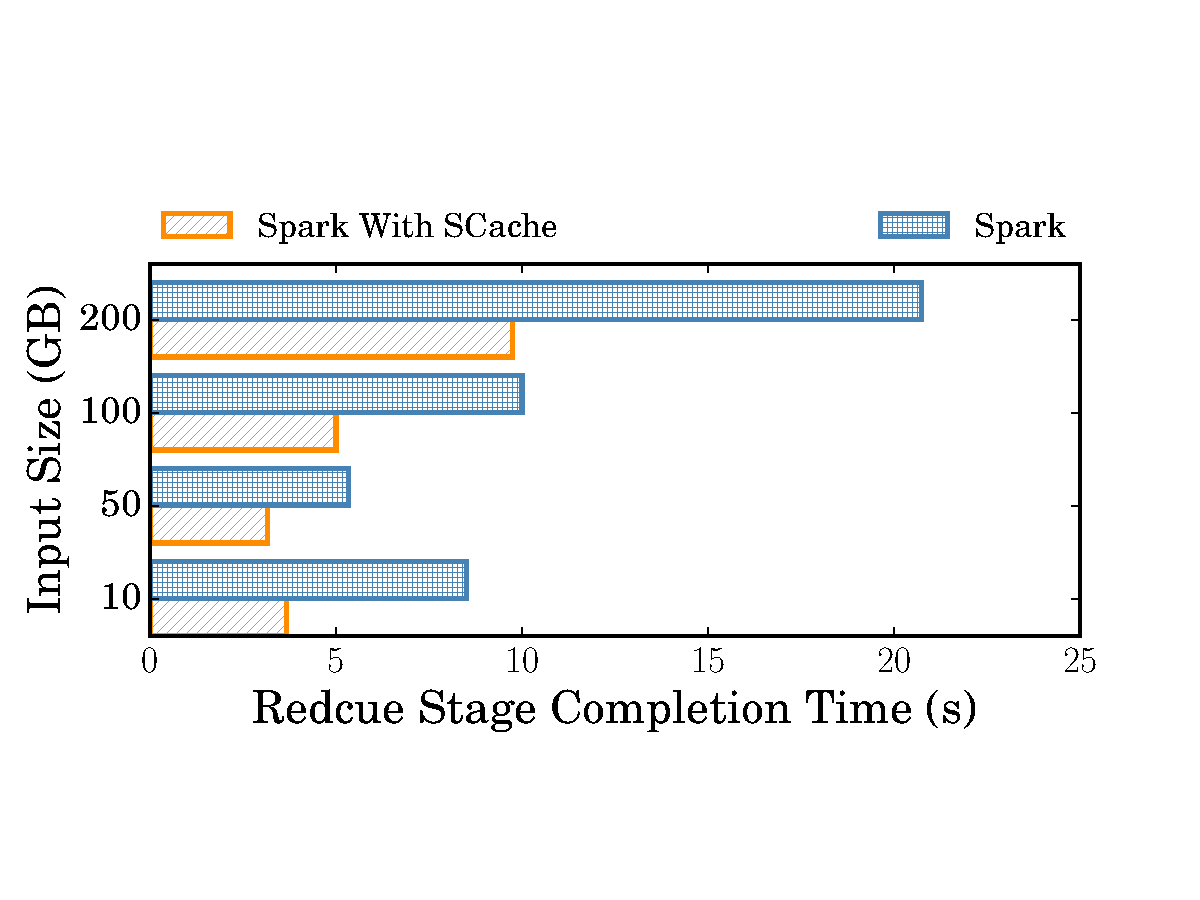
\includegraphics[width=0.8\linewidth]{fig/tera}
% 				\caption{Reduce Stage Completion Time Comparsion}
% 				\label{fig:terasort}
% 			\end{subfigure}
% 			\begin{subfigure}{0.5\textwidth}
% 				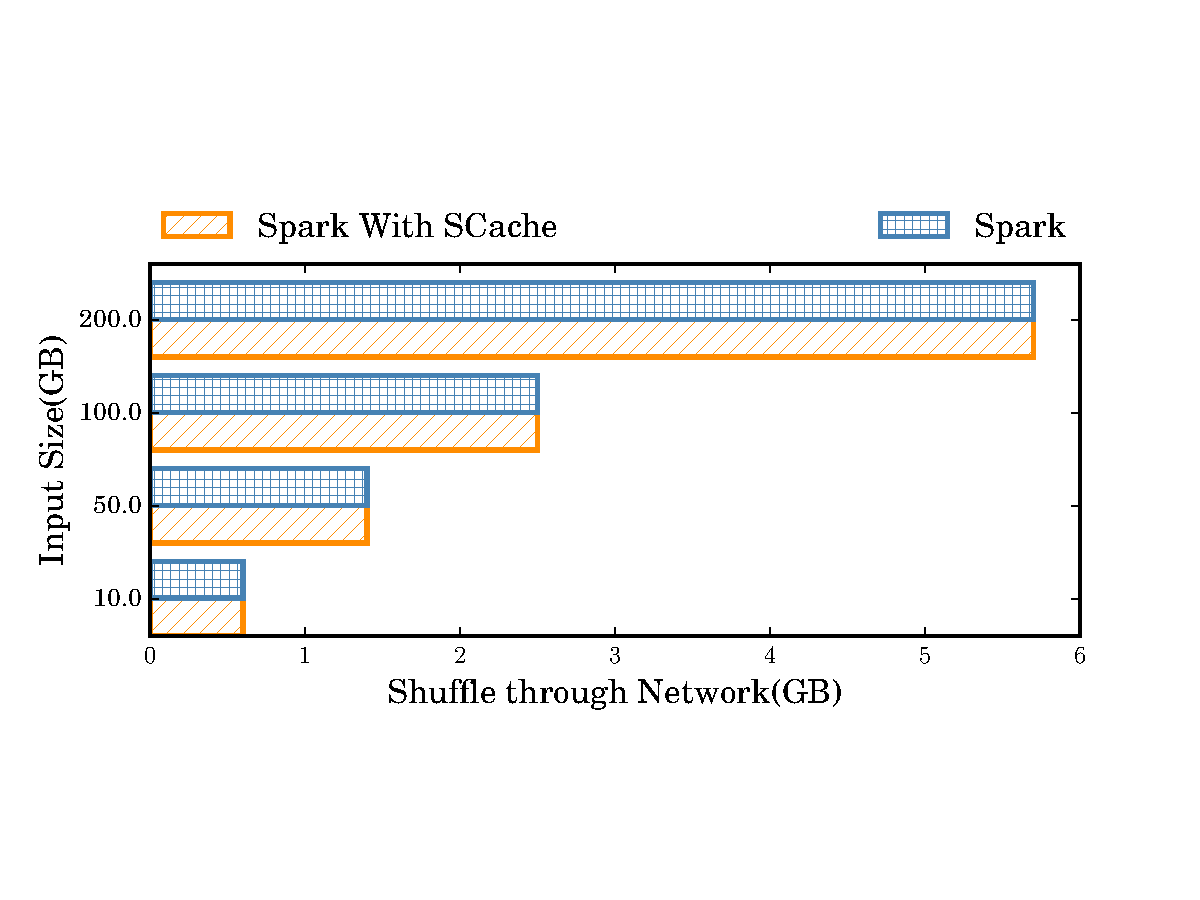
\includegraphics[width=0.8\linewidth]{fig/tera_shuffle}
% 				\caption{Shuffle Data Size Comparsion}
% 				\label{fig:terashuffle}
% 			\end{subfigure}
% 			\caption{Terasort Evaluation}
% 		\end{figure}
		
% 	\end{minipage}
%  \end{figure*}

% \begin{figure}
% \begin{subfigure}{\linewidth}
% 	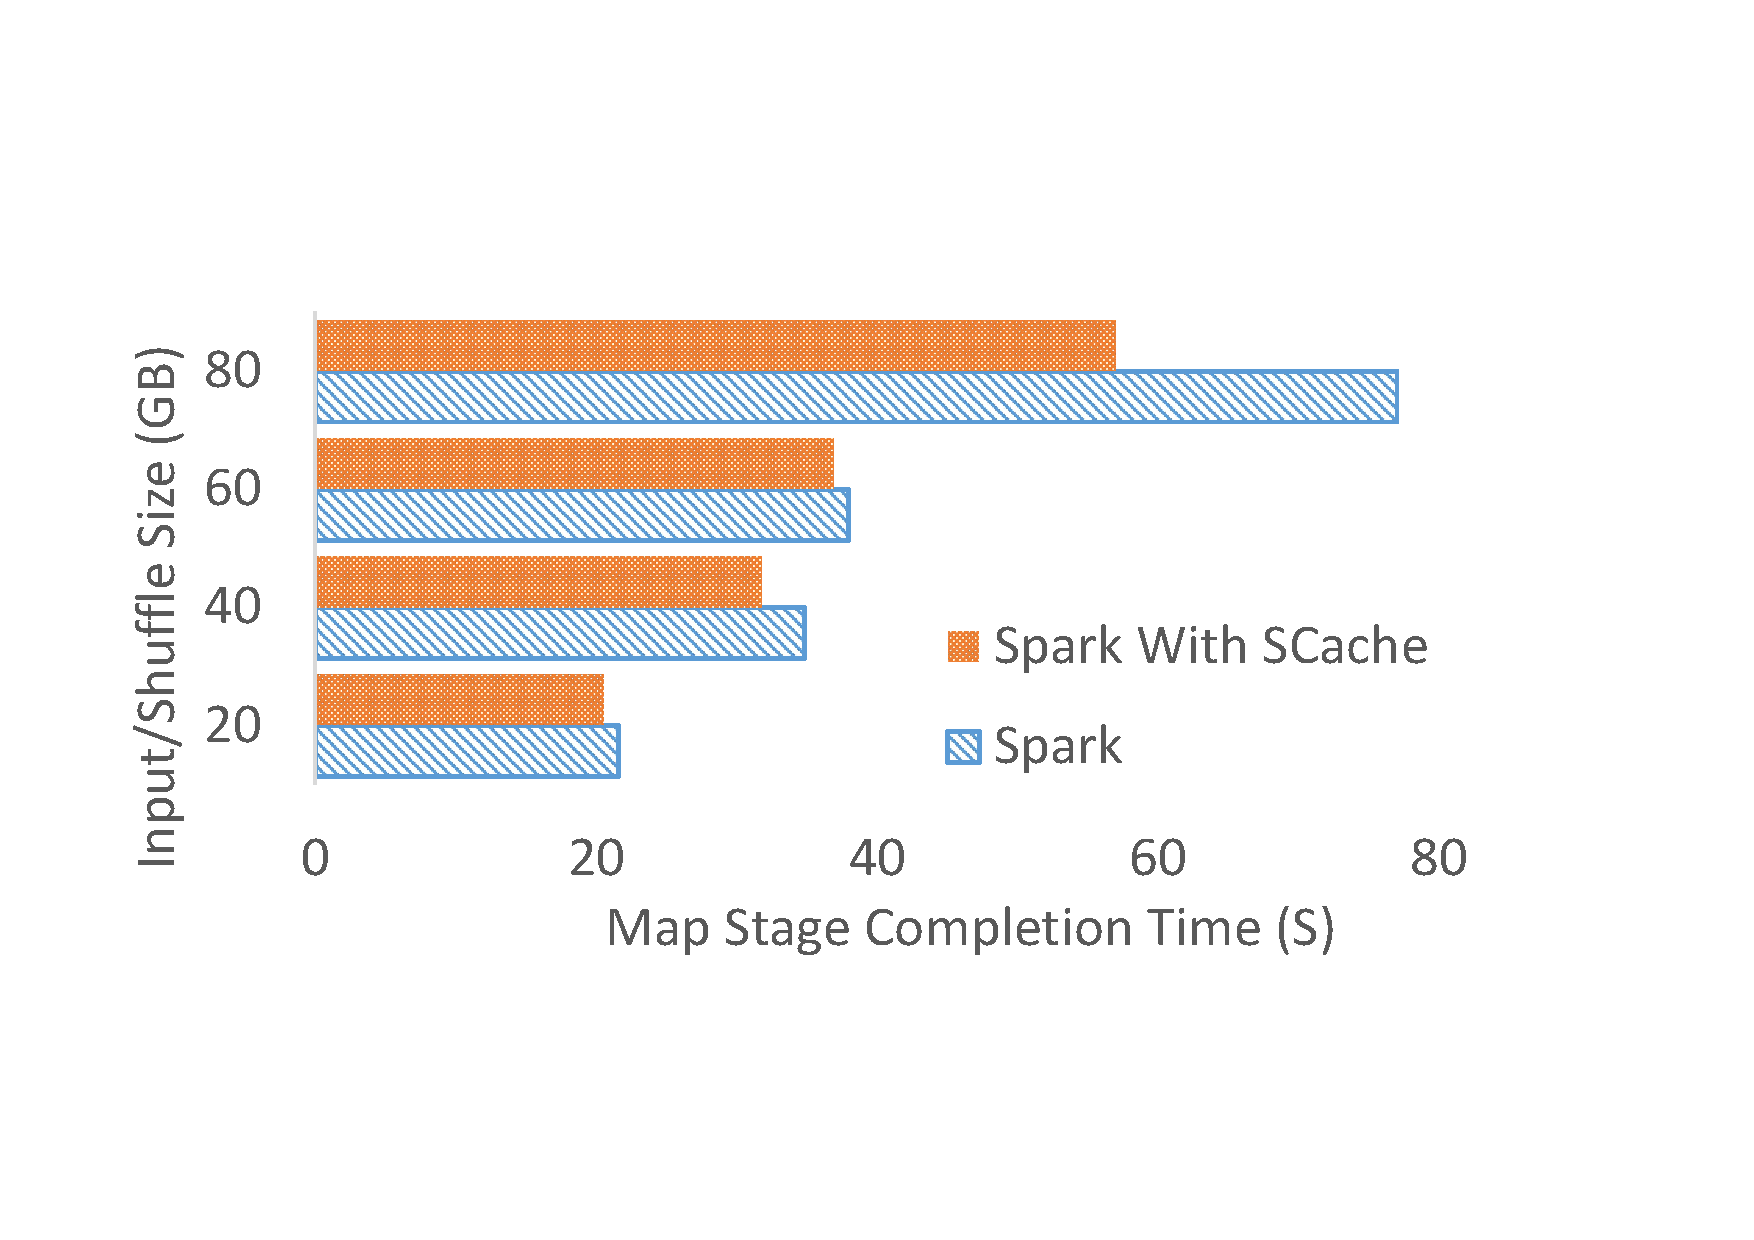
\includegraphics[width=\linewidth]{fig/groupbymapstage}
% 	\caption{Map Stage Completion Time Comparsion}
% 	\label{fig:mapstage}
% \end{subfigure}
% \begin{subfigure}{\linewidth}
% 	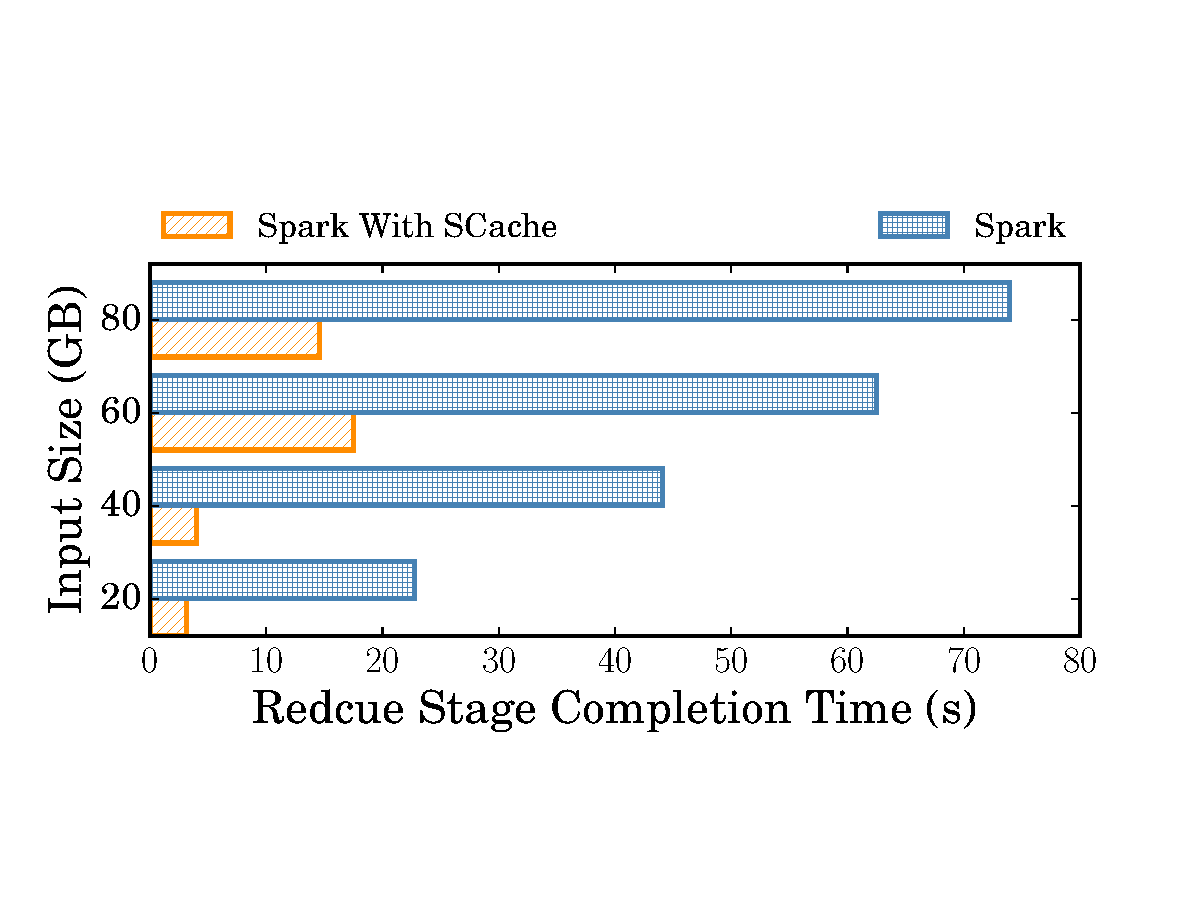
\includegraphics[width=\linewidth]{fig/groupbyreducestage}
% 	\caption{Reduce Stage Completion Time Comparsion}
% 	\label{fig:reducestage}
% \end{subfigure}
% \caption{Stage Completion Time Comparsion of Single Shuffle Test}
% \label{fig:singleshuffle}
% \end{figure}
\subsection{Terasort}
In this part, we evaluate the Terasort \cite{spark-tera}.
Terasort \cite{spark-tera} is a shuffle intensive benchmark for distributed system analysis. It consists of two consecutive shuffles. The first shuffle reads the input data and uses a customized hash partition function for re-partitioning. The second shuffle partitions the data through a range partitioner. As the range bounds set by range partitioner almost match the same pattern of the first shuffle, almost $93\%$ of input data is from one particular map task for each reduce task. It makes the shuffle data transferred through network extremely small under Spark locality preferred task scheduling. So we take the second shuffle as an extreme case to evaluate the scheduling locality for SCache.

As shown in Figure \ref{fig:terasort}, we present the first shuffle as the evaluation of shuffle optimization. At the same time, we use the second the shuffle to evaluate in the dimension of scheduling locality (Figure \ref{fig:terashuffle}). For the first shuffle, Spark with SCache runs 2 $\times$ faster during the reduce stage with the input data in a range from 10GB to 200GB. At the same time, Figure \ref{fig:terashuffle} reveals that SCache pre-scheduling produces exactly same network traffic of second shuffle as Spark, which implies that SCache pre-scheduling can obtain the best locality while balancing the load. In contrast, Spark delays scheduling reduce tasks with the shuffle map output to achieve this optimum.

\subsection{Production Workload}
We also evaluate some shuffle heavy queries from TPC-DS \cite{tpcds}. TPC-DS benchmark is designed for modeling multiple users submitting varied queries (e.g. ad-hoc, interactive OLAP, data mining, etc.). TPC-DS contains 99 queries and is considered as the standardized industry benchmark for testing big data systems. We evaluate the performance of Spark with SCache by picking some of the TPC-DS queries with shuffle intensive attribute. As shown in Figure \ref{fig:tpcds}, on the horizontal axis is query number, and on the vertical axis is query completion time. Spark with SCache outperforms the original Spark in almost all the queries. Furthermore, in many queries, Spark with SCache outperforms original Spark by an order of magnitude. The overall reduction portion of query time that SCache achieved is 40\% on average. Since this evaluation presents the overall job completion time of queries, we believe that our shuffle optimization is promising.
\begin{figure}
	\begin{subfigure}{\linewidth}
		\centering
		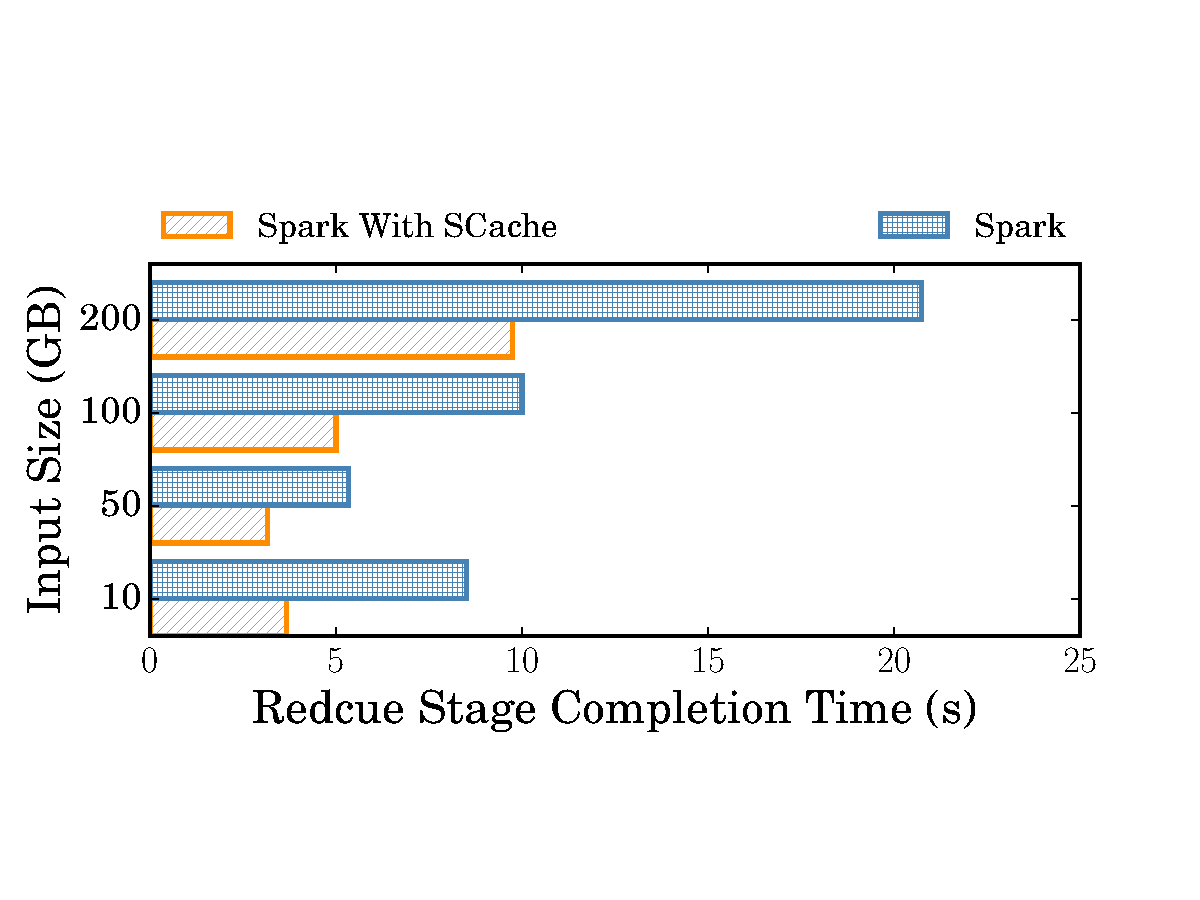
\includegraphics[width=0.915\linewidth]{fig/tera}
		\caption{Reduce Stage Completion Time Comparison of First Shuffle}
		\label{fig:terasort}
	\end{subfigure}
	\vspace{0.08cm}
	\begin{subfigure}{\linewidth}
		\centering
		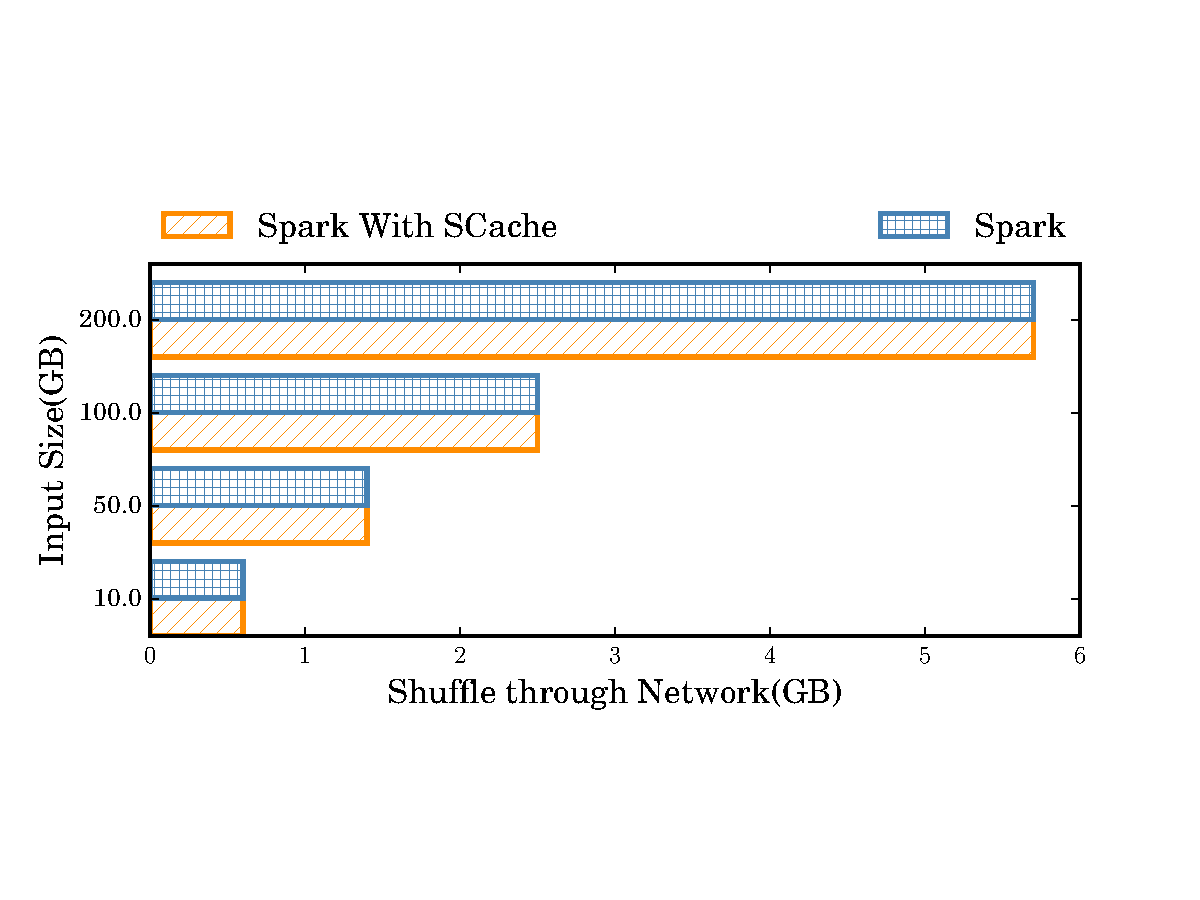
\includegraphics[width=0.915\linewidth]{fig/tera_shuffle}
		\caption{Shuffle Data throuth Network Comparison of Second Shuffle}
		\label{fig:terashuffle}
	\end{subfigure}
	\caption{Terasort Evaluation}
\end{figure}
\subsection{Overhead of Sampling}
In this part, we evaluate the overhead of sampling with different input data sizes on one node and cluster scales. In \ref{fig:sampling}, the overhead of sampling only grows with the increase of input size on each node. But it remains relatively stable when the cluster size scales up. It makes SCache a scalable system in cluster.
\begin{figure*}
	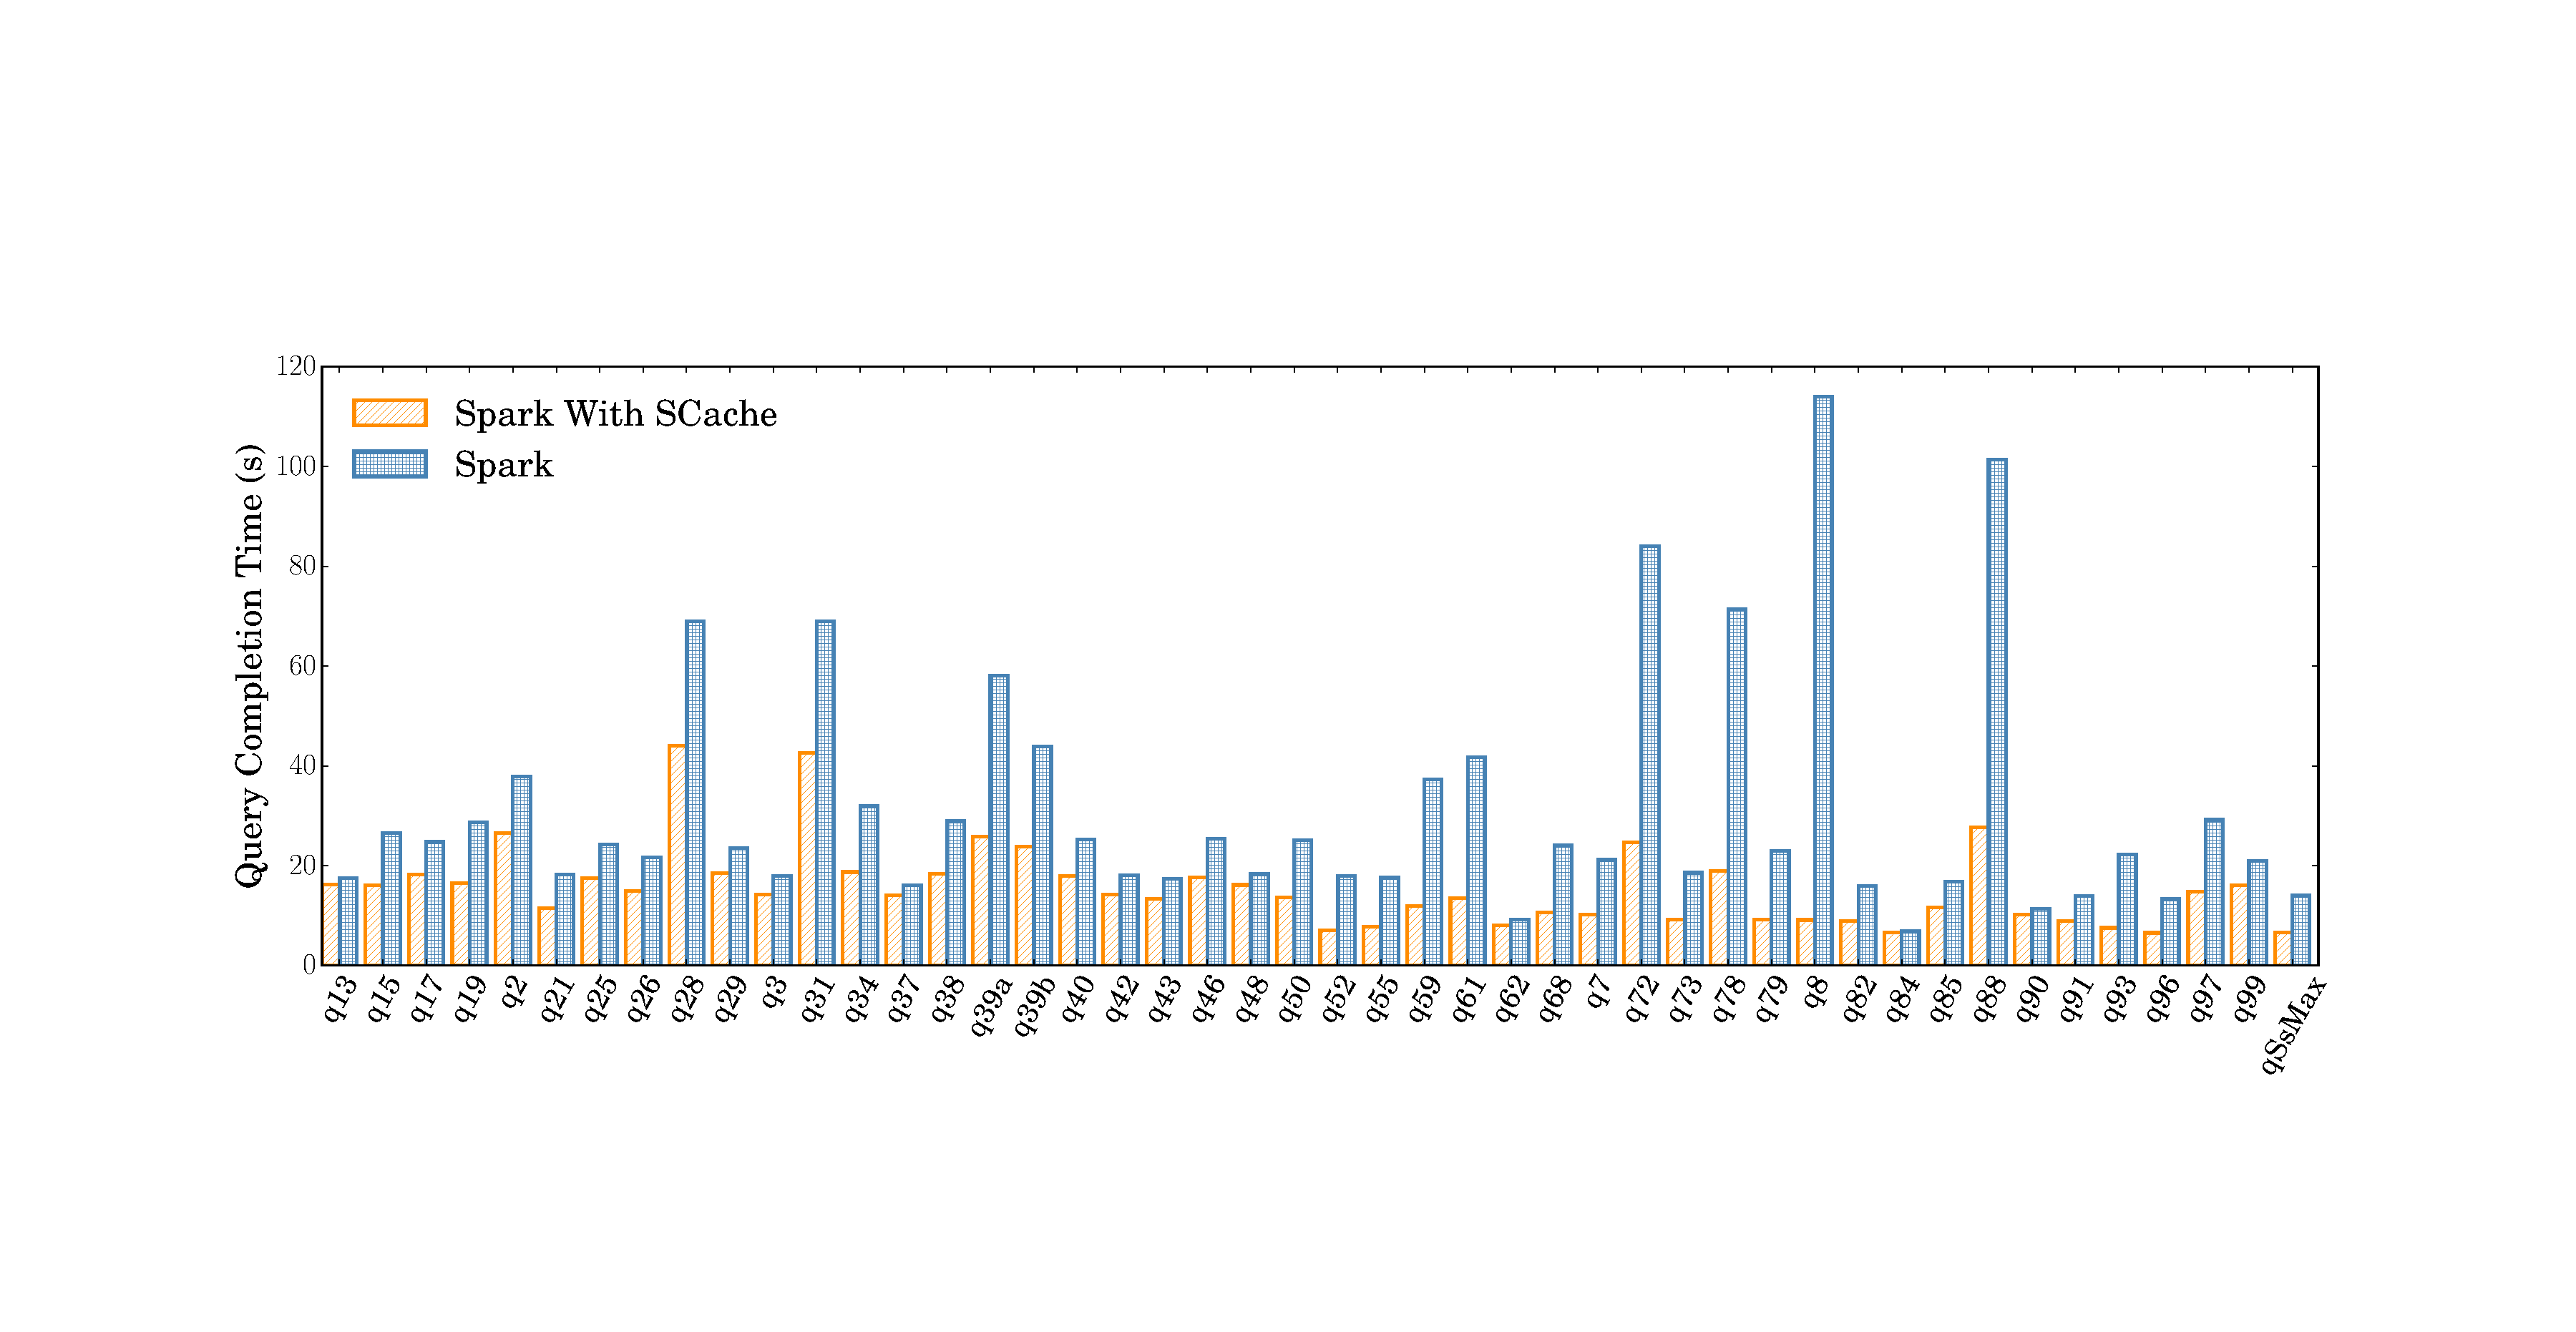
\includegraphics[width=\textwidth]{fig/tpcds}
	\caption{TPC-DS Benchmark Evaluation}
	\label{fig:tpcds}
\end{figure*}



% %# -*- coding: utf-8-unix -*-
%%==================================================
%% chapter02.tex for SJTU Master Thesis
%% based on CASthesis
%% modified by wei.jianwen@gmail.com
%% Encoding: UTF-8
%%==================================================

\chapter{ \LaTeX 排版例子}
\label{chap:example}

\section{列表环境}
\label{sec:list}

\subsection{无序列表}
\label{sec:unorderlist}

以下是一个无序列表的例子,列表的每个条目单独分段。

\begin{itemize}
  \item 这是一个无序列表。
  \item 这是一个无序列表。
  \item 这是一个无序列表。
\end{itemize}

使用\verb+itemize*+环境可以创建行内无序列表。
\begin{itemize*}
  \item 这是一个无序列表。
  \item 这是一个无序列表。
  \item 这是一个无序列表。
\end{itemize*}
行内无序列表条目不单独分段,所有内容直接插入在原文的段落中。

\subsection{有序列表}
\label{sec:orderlist}

使用环境\verb+enumerate+和\verb+enumerate*+创建有序列表,
使用方法无序列表类似。

\begin{enumerate}
  \item 这是一个有序列表。
  \item 这是一个有序列表。
  \item 这是一个有序列表。
\end{enumerate}

使用\verb+enumerate*+环境可以创建行内有序列表。
\begin{enumerate*}
  \item 这是一个默认有序列表。
  \item 这是一个默认有序列表。
  \item 这是一个默认有序列表。
\end{enumerate*}
行内有序列表条目不单独分段,所有内容直接插入在原文的段落中。

\subsection{描述型列表}

使用环境\verb+description+可创建带有主题词的列表,条目语法是\verb+\item[主题] 内容+。
\begin{description}
    \item[主题一] 详细内容
    \item[主题二] 详细内容
    \item[主题三] 详细内容 \ldots
\end{description}

\subsection{自定义列表样式}

可以使用\verb+label+参数控制列表的样式,
详细可以参考WikiBooks\footnote{\url{https://en.wikibooks.org/wiki/LaTeX/List_Structures\#Customizing_lists}}。
比如一个自定义样式的行内有序列表
\begin{enumerate*}[label=\itshape\alph*)\upshape]
  \item 这是一个自定义样式有序列表。
  \item 这是一个自定义样式有序列表。
  \item 这是一个自定义样式有序列表。
\end{enumerate*}

\section{数学排版}
\label{sec:matheq}

\subsection{公式排版}
\label{sec:eqformat}

这里有举一个长公式排版的例子,来自\href{http://www.tex.ac.uk/tex-archive/info/math/voss/mathmode/Mathmode.pdf}{《Math mode》}:

\begin {multline}
  \frac {1}{2}\Delta (f_{ij}f^{ij})=
  2\left (\sum _{i<j}\chi _{ij}(\sigma _{i}-
    \sigma _{j}) ^{2}+ f^{ij}\nabla _{j}\nabla _{i}(\Delta f)+\right .\\
  \left .+\nabla _{k}f_{ij}\nabla ^{k}f^{ij}+
    f^{ij}f^{k}\left [2\nabla _{i}R_{jk}-
      \nabla _{k}R_{ij}\right ]\vphantom {\sum _{i<j}}\right )
\end{multline}

\subsection{SI单位}

使用\verb+siunitx+宏包可以方便地输入SI单位制单位,例如\verb+\SI{5}{\um}+可以得到\SI{5}{\um}。

\subsubsection{一个四级标题}
\label{sec:depth4}

这是全文唯一的一个四级标题。在这部分中将演示了mathtools宏包中可伸长符号(箭头、等号的例子)的例子。

\begin{displaymath}
    A \xleftarrow[n=0]{} B \xrightarrow[LongLongLongLong]{n>0} C 
\end{displaymath}

\begin{eqnarray}
  f(x) & \xleftrightarrow[]{A=B}  & B \\
  & \xleftharpoondown[below]{above} & B \nonumber \\
  & \xLeftrightarrow[below]{above} & B
\end{eqnarray}

又如:

\begin{align}
  \label{eq:none}
  & I(X_3;X_4)-I(X_3;X_4\mid{}X_1)-I(X_3;X_4\mid{}X_2) \nonumber \\
  = & [I(X_3;X_4)-I(X_3;X_4\mid{}X_1)]-I(X_3;X_4\mid{}\tilde{X}_2) \\
  = & I(X_1;X_3;X_4)-I(X_3;X_4\mid{}\tilde{X}_2)
\end{align}

\subsection{定理环境}

模板中定义了丰富的定理环境
algo(算法),thm(定理),lem(引理),prop(命题),cor(推论),defn(定义),conj(猜想),exmp(例),rem(注),case(情形),
bthm(断言定理),blem(断言引理),bprop(断言命题),bcor(断言推论)。
amsmath还提供了一个proof(证明)的环境。
这里举一个“定理”和“证明”的例子。
\begin{thm}[留数定理]
\label{thm:res}
  假设$U$是复平面上的一个单连通开子集,$a_1,\ldots,a_n$是复平面上有限个点,$f$是定义在$U\backslash \{a_1,\ldots,a_n\}$上的全纯函数,
  如果$\gamma$是一条把$a_1,\ldots,a_n$包围起来的可求长曲线,但不经过任何一个$a_k$,并且其起点与终点重合,那么:

  \begin{equation}
    \label{eq:res}
    \ointop_{\gamma}f(z)\,\mathrm{d}z = 2\uppi\mathbf{i}\sum^n_{k=1}\mathrm{I}(\gamma,a_k)\mathrm{Res}(f,a_k)
  \end{equation}

  如果$\gamma$是若尔当曲线,那么$\mathrm{I}(\gamma, a_k)=1$,因此:

  \begin{equation}
    \label{eq:resthm}
    \ointop_{\gamma}f(z)\,\mathrm{d}z = 2\uppi\mathbf{i}\sum^n_{k=1}\mathrm{Res}(f,a_k)
  \end{equation}

      % \oint_\gamma f(z)\, dz = 2\pi i \sum_{k=1}^n \mathrm{Res}(f, a_k ). 

  在这里,$\mathrm{Res}(f, a_k)$表示$f$在点$a_k$的留数,$\mathrm{I}(\gamma,a_k)$表示$\gamma$关于点$a_k$的卷绕数。
  卷绕数是一个整数,它描述了曲线$\gamma$绕过点$a_k$的次数。如果$\gamma$依逆时针方向绕着$a_k$移动,卷绕数就是一个正数,
  如果$\gamma$根本不绕过$a_k$,卷绕数就是零。

  定理\ref{thm:res}的证明。
  
  \begin{proof}
    首先,由……

    其次,……

    所以……
  \end{proof}
\end{thm}

上面的公式例子中,有一些细节希望大家注意。微分号d应该使用“直立体”也就是用mathrm包围起来。
并且,微分号和被积函数之间应该有一段小间隔,可以插入\verb+\,+得到。
斜体的$d$通常只作为一般变量。
i,j作为虚数单位时,也应该使用“直立体”为了明显,还加上了粗体,例如\verb+\mathbf{i}+。斜体$i,j$通常用作表示“序号”。
其他字母在表示常量时,也推荐使用“直立体”譬如,圆周率$\uppi$(需要upgreek宏包),自然对数的底$\mathrm{e}$。
不过,我个人觉得斜体的$e$和$\pi$很潇洒,在不至于引起混淆的情况下,我也用这两个字母的斜体表示对应的常量。


\section{向文档中插入图像}
\label{sec:insertimage}

\subsection{支持的图片格式}
\label{sec:imageformat}

\XeTeX 可以很方便地插入PDF、PNG、JPG格式的图片。

插入PNG/JPG的例子如\ref{fig:SRR}所示。
这两个水平并列放置的图共享一个“图标题”(table caption),没有各自的小标题。

\begin{figure}[!htp]
  \centering
  
\includegraphics[width=0.3\textwidth]{example/sjtulogo.png}
  \hspace{1cm}
  
\includegraphics[width=0.3\textwidth]{example/sjtulogo.jpg}
  \bicaption[fig:SRR]{这里将出现在插图索引中}{中文题图}{Fig}{English caption}
\end{figure}

% 这里还有插入eps图像和pdf图像的例子,如图\ref{fig:epspdf:a}和图\ref{fig:epspdf:b}。这里将EPS和PDF图片作为子图插入,每个子图有自己的小标题。并列子图的功能是使用subfigure宏包提供的。
% 
% \begin{figure}
%   \centering
%   \subfigure[EPS Figure]{
%     \label{fig:epspdf:a} %% label for first subfigure
%     
\includegraphics[width=0.3\textwidth]{example/sjtulogo.eps}}
%   \hspace{1in}
%   \subfigure[PDF Figure]{
%     \label{fig:epspdf:b} %% label for second subfigure
%     
\includegraphics[width=0.3\textwidth]{example/sjtulogo.pdf}}
%   \bicaption[fig:pdfeps]{插入eps图像和pdf图像}{插入eps和pdf的例子}{Fig}{An EPS and PDF demo}
% \end{figure}

更多关于 \LaTeX 插图的例子可以参考\href{http://www.cs.duke.edu/junhu/Graphics3.pdf}{《\LaTeX 插图指南》}。

\subsection{长标题的换行}
\label{sec:longcaption}

图\ref{fig:longcaptionbad}和图\ref{fig:longcaptiongood}都有比较长图标题,通过对比发现,图\ref{fig:longcaptiongood}的换行效果更好一些。
其中使用了minipage环境来限制整个浮动体的宽度。

\begin{figure}[!htp]
 \centering
 
\includegraphics[width=4cm]{example/sjtulogo.pdf}
 \bicaption[fig:longcaptionbad]{这里将出现在插图索引}{海交通大学是我国历史最悠久的高等学府之一,是教育部直属、教育部与上海市共建的全国重点大学.}{Fig}{Where there is a will, there is a way.}
\end{figure}

\begin{figure}[!htbp]
  \centering
  \begin{minipage}[b]{0.6\textwidth}
    \captionstyle{\centering}
    \centering
    
\includegraphics[width=4cm]{example/sjtulogo.pdf}
    \bicaption[fig:longcaptiongood]{这里将出现在插图索引}{海交通大学是我国历史最悠久的高等学府之一,是教育部直属、教育部与上海市共建的全国重点大学.}{Fig}{Where there is a will, there is a way.}
  \end{minipage}     
\end{figure}

\subsection{绘制流程图}

图\ref{fig:flow_chart}是一张流程图示意。使用tikz环境,搭配四种预定义节点(\verb+startstop+、\verb+process+、\verb+decision+和\verb+io+),可以容易地绘制出流程图。
\begin{figure}[!htp]
    \centering
    \resizebox{6cm}{!}{\begin{tikzpicture}[node distance=2cm]
    \node (pic) [startstop] {待测图片};
    \node (bg) [io, below of=pic] {读取背景};
    \node (pair) [process, below of=bg] {匹配特征点对};
    \node (threshold) [decision, below of=pair, yshift=-0.5cm] {多于阈值};
    \node (clear) [decision, right of=threshold, xshift=3cm] {清晰?};
    \node (capture) [process, right of=pair, xshift=3cm, yshift=0.5cm] {重采};
    \node (matrix_p) [process, below of=threshold, yshift=-0.8cm] {透视变换矩阵};
    \node (matrix_a) [process, right of=matrix_p, xshift=3cm] {仿射变换矩阵};
    \node (reg) [process, below of=matrix_p] {图像修正};
    \node (return) [startstop, below of=reg] {配准结果};
     
    %连接具体形状
    \draw [arrow](pic) -- (bg);
    \draw [arrow](bg) -- (pair);
    \draw [arrow](pair) -- (threshold);

    \draw [arrow](threshold) -- node[anchor=south] {否} (clear);

    \draw [arrow](clear) -- node[anchor=west] {否} (capture);
    \draw [arrow](capture) |- (pic);
    \draw [arrow](clear) -- node[anchor=west] {是} (matrix_a);
    \draw [arrow](matrix_a) |- (reg);

    \draw [arrow](threshold) -- node[anchor=east] {是} (matrix_p);
    \draw [arrow](matrix_p) -- (reg);
    \draw [arrow](reg) -- (return);
\end{tikzpicture}
}
    \bicaption[fig:flow_chart]{绘制流程图效果}{流程图}{Fig}{Flow chart}
\end{figure}
  
\clearpage

\section{表格}
\label{sec:tab}

这一节给出的是一些表格的例子,如表\ref{tab:firstone}所示。

\begin{table}[!hpb]
  \centering
  \bicaption[tab:firstone]{指向一个表格的表目录索引}{一个颇为标准的三线表格\footnotemark[1]}{Table}{A Table}
  \begin{tabular}{@{}llr@{}} \toprule
    \multicolumn{2}{c}{Item} \\ \cmidrule(r){1-2}
    Animal & Description & Price (\$)\\ \midrule
    Gnat & per gram & 13.65 \\
    & each & 0.01 \\
    Gnu & stuffed & 92.50 \\
    Emu & stuffed & 33.33 \\
    Armadillo & frozen & 8.99 \\ \bottomrule
  \end{tabular}
\end{table}
\footnotetext[1]{这个例子来自\href{http://www.ctan.org/tex-archive/macros/latex/contrib/booktabs/booktabs.pdf}{《Publication quality tables in LATEX》}(booktabs宏包的文档)。这也是一个在表格中使用脚注的例子,请留意与threeparttable实现的效果有何不同。}

下面一个是一个更复杂的表格,用threeparttable实现带有脚注的表格,如表\ref{tab:footnote}。

\begin{table}[!htpb]
  \bicaption[tab:footnote]{出现在表目录的标题}{一个带有脚注的表格的例子}{Table}{A Table with footnotes}
  \centering
  \begin{threeparttable}[b]
     \begin{tabular}{ccd{4}cccc}
      \toprule
      \multirow{2}{6mm}{total}&\multicolumn{2}{c}{20\tnote{1}} & \multicolumn{2}{c}{40} &  \multicolumn{2}{c}{60}\\
      \cmidrule(lr){2-3}\cmidrule(lr){4-5}\cmidrule(lr){6-7}
      &www & k & www & k & www & k \\
      \midrule
      &$\underset{(2.12)}{4.22}$ & 120.0140\tnote{2} & 333.15 & 0.0411 & 444.99 & 0.1387 \\
      &168.6123 & 10.86 & 255.37 & 0.0353 & 376.14 & 0.1058 \\
      &6.761    & 0.007 & 235.37 & 0.0267 & 348.66 & 0.1010 \\
      \bottomrule
    \end{tabular}
    \begin{tablenotes}
    \item [1] the first note.% or \item [a]
    \item [2] the second note.% or \item [b]
    \end{tablenotes}
  \end{threeparttable}
\end{table}

\section{参考文献管理}

 \LaTeX 具有将参考文献内容和表现形式分开管理的能力,涉及三个要素:参考文献数据库、参考文献引用格式、在正文中引用参考文献。
这样的流程需要多次编译:

\begin{enumerate}[noitemsep,topsep=0pt,parsep=0pt,partopsep=0pt]
	\item 用户将论文中需要引用的参考文献条目,录入纯文本数据库文件(bib文件)。
	\item 调用xelatex对论文模板做第一次编译,扫描文中引用的参考文献,生成参考文献入口文件(aux)文件。
	\item 调用bibtex,以参考文献格式和入口文件为输入,生成格式化以后的参考文献条目文件(bib)。
	\item 再次调用xelatex编译模板,将格式化以后的参考文献条目插入正文。
\end{enumerate}

参考文献数据库(thesis.bib)的条目,可以从Google Scholar搜索引擎\footnote{\url{https://scholar.google.com}}、CiteSeerX搜索引擎\footnote{\url{http://citeseerx.ist.psu.edu}}中查找,文献管理软件Papers\footnote{\url{http://papersapp.com}}、Mendeley\footnote{\url{http://www.mendeley.com}}、JabRef\footnote{\url{http://jabref.sourceforge.net}}也能够输出条目信息。

下面是在Google Scholar上搜索到的一条文献信息,格式是纯文本:

\begin{lstlisting}[caption={从Google Scholar找到的参考文献条目}, label=googlescholar, escapeinside="", numbers=none]
    @phdthesis{"白2008信用风险传染模型和信用衍生品的定价",
      title={"信用风险传染模型和信用衍生品的定价"},
      author={"白云芬"},
      year={2008},
      school={"上海交通大学"}
    } 
\end{lstlisting}

推荐修改后在bib文件中的内容为:

\begin{lstlisting}[caption={修改后的参考文献条目}, label=itemok, escapeinside="", numbers=none]
  @phdthesis{bai2008,
    title={"信用风险传染模型和信用衍生品的定价"},
    author={"白云芬"},
    date={2008},
    address={"上海"},
    school={"上海交通大学"}
  } 
\end{lstlisting}

按照教务处的要求,参考文献外观应符合国标GBT7714的要求\footnote{\url{http://www.cces.net.cn/guild/sites/tmxb/Files/19798_2.pdf}}。
在模板中,表现形式的控制逻辑通过bibla­tex-gb7714-2015包实现\footnote{\url{https://www.ctan.org/pkg/biblatex-gb7714-2015}},基于{Bib\LaTeX}管理文献。在目前的多数TeX发行版中,可能都没有默认包含biblatex-gb7714-2015,需要手动安装。

正文中引用参考文献时,用\verb+\cite{key1,key2,key3...}+可以产生“上标引用的参考文献”,
如\cite{Meta_CN,chen2007act,DPMG}。
使用\verb+\citen{key1,key2,key3...}+则可以产生水平引用的参考文献,例如\citen{JohnD,zhubajie,IEEE-1363}。
请看下面的例子,将会穿插使用水平的和上标的参考文献:关于书的\citen{Meta_CN,JohnD,IEEE-1363},关于期刊的\cite{chen2007act,chen2007ewi},
会议论文\citen{DPMG,kocher99,cnproceed},
硕士学位论文\citen{zhubajie,metamori2004},博士学位论文\cite{shaheshang,FistSystem01,bai2008},标准文件\citen{IEEE-1363},技术报告\cite{NPB2},电子文献\citen{xiaoyu2001, CHRISTINE1998},用户手册\citen{RManual}。

总结一些注意事项:
\begin{itemize}
\item 参考文献只有在正文中被引用了,才会在最后的参考文献列表中出现;
\item 参考文献“数据库文件”bib是纯文本文件,请使用UTF-8编码,不要使用GBK编码;
\item 参考文献条目中默认通过date域输入时间。兼容使用year域时会产生编译warning,可忽略。
\end{itemize}

\section{用listings插入源代码}

原先ctexbook文档类和listings宏包配合使用时,代码在换页时会出现莫名其妙的错误,后来经高人指点,顺利解决了。
感兴趣的话,可以看看\href{http://bbs.ctex.org/viewthread.php?tid=53451}{这里}。
这里给使用listings宏包插入源代码的例子,这里是一段C代码。
另外,listings宏包真可谓博大精深,可以实现各种复杂、漂亮的效果,想要进一步学习的同学,可以参考
\href{http://mirror.ctan.org/macros/latex/contrib/listings/listings.pdf}{listings宏包手册}。

\begin{lstlisting}[language={C}, caption={一段C源代码}]
#include <stdio.h>
#include <unistd.h>
#include <sys/types.h>
#include <sys/wait.h>

int main() {
  pid_t pid;

  switch ((pid = fork())) {
  case -1:
    printf("fork failed\n");
    break;
  case 0:
    /* child calls exec */
    execl("/bin/ls", "ls", "-l", (char*)0);
    printf("execl failed\n");
    break;
  default:
    /* parent uses wait to suspend execution until child finishes */
    wait((int*)0);
    printf("is completed\n");
    break;
  }

  return 0;
}
\end{lstlisting}

\section{用algorithm和algorithmicx宏包插入算法描述}

algorithmicx 比 algorithmic 增加了一些命令。
示例如算法\ref{algo:sum_100}和算法\ref{algo:merge_sort},
后者的代码来自\href{http://hustsxh.is-programmer.com/posts/38801.html}{xhSong的博客}。
algorithmicx的详细使用方法见\href{http://mirror.hust.edu.cn/CTAN/macros/latex/contrib/algorithmicx/algorithmicx.pdf}{官方README}。
使用算法宏包时,算法出现的位置很多时候不按照tex文件里的书写顺序, 
需要强制定位时可以使用\verb+\begin{algorithm}[H]+
\footnote{http://tex.stackexchange.com/questions/165021/fixing-the-location-of-the-appearance-in-algorithmicx-environment}

这是写在算法\ref{algo:sum_100}前面的一段话,在生成的文件里它会出现在算法\ref{algo:sum_100}前面。

\begin{algorithm}
% \begin{algorithm}[H] % 强制定位
\caption{求100以内的整数和}
\label{algo:sum_100}
\begin{algorithmic}[1] %每行显示行号
\Ensure 100以内的整数和 % 输出
\State $sum \gets 0$
\For{$i = 0 \to 100$}
    \State $sum \gets sum + i$
  \EndFor
\end{algorithmic}
\end{algorithm}

这是写在两个算法中间的一段话,当算法\ref{algo:sum_100}不使用\verb+\begin{algorithm}[H]+时它也会出现在算法\ref{algo:sum_100}前面。

对于很长的算法,单一的算法块\verb+\begin{algorithm}...\end{algorithm}+是不能自动跨页的
\footnote{http://tex.stackexchange.com/questions/70733/latex-algorithm-not-display-under-correct-section},
会出现的情况有:

\begin{itemize}
  \item 该页放不下当前的算法,留下大片空白,算法在下一页显示
  \item 单一页面放不下当前的算法,显示时超过页码的位置直到超出整个页面范围
\end{itemize}

解决方法有:

\begin{itemize}
  \item (推荐)使用\verb+algstore{algname}+和\verb+algrestore{algname}+来讲算法分为两个部分\footnote{http://tex.stackexchange.com/questions/29816/algorithm-over-2-pages},如算法\ref{algo:merge_sort}。
  \item 人工拆分算法为多个小的部分。
\end{itemize}

\begin{algorithm}
% \begin{algorithm}[H] % 强制定位
\caption{用归并排序求逆序数}
\label{algo:merge_sort}
\begin{algorithmic}[1] %每行显示行号
\Require $Array$数组,$n$数组大小 % 输入
\Ensure 逆序数 % 输出
\Function {MergerSort}{$Array, left, right$}
  \State $result \gets 0$
  \If {$left < right$}
    \State $middle \gets (left + right) / 2$
    \State $result \gets result +$ \Call{MergerSort}{$Array, left, middle$}
    \State $result \gets result +$ \Call{MergerSort}{$Array, middle, right$}
    \State $result \gets result +$ \Call{Merger}{$Array,left,middle,right$}
  \EndIf
  \State \Return{$result$}
\EndFunction
\State %空一行
\Function{Merger}{$Array, left, middle, right$}
  \State $i\gets left$
  \State $j\gets middle$
  \State $k\gets 0$
  \State $result \gets 0$
  \While{$i<middle$ \textbf{and} $j<right$}
    \If{$Array[i]<Array[j]$}
      \State $B[k++]\gets Array[i++]$
    \Else
      \State $B[k++] \gets Array[j++]$
      \State $result \gets result + (middle - i)$
    \EndIf
  \EndWhile
  \algstore{MergeSort}
\end{algorithmic}
\end{algorithm}

\begin{algorithm}
\begin{algorithmic}[1]
  \algrestore{MergeSort}
  \While{$i<middle$}
    \State $B[k++] \gets Array[i++]$
  \EndWhile
  \While{$j<right$}
    \State $B[k++] \gets Array[j++]$
  \EndWhile
  \For{$i = 0 \to k-1$}
    \State $Array[left + i] \gets B[i]$
  \EndFor
  \State \Return{$result$}
\EndFunction
\end{algorithmic}
\end{algorithm}

这是写在算法\ref{algo:merge_sort}后面的一段话,
但是当算法\ref{algo:merge_sort}不使用\verb+\begin{algorithm}[H]+时它会出现在算法\ref{algo:merge_sort}
甚至算法\ref{algo:sum_100}前面。

对于算法的索引要注意\verb+\caption+和\verb+\label+的位置, 
必须是先\verb+\caption+再\verb+\label+\footnote{http://tex.stackexchange.com/questions/65993/algorithm-numbering},
否则会出现\verb+\ref{algo:sum_100}+生成的编号跟对应算法上显示不一致的问题。

根据Werner的回答\footnote{http://tex.stackexchange.com/questions/53357/switch-cases-in-algorithmic}
增加了\verb+Switch+和\verb+Case+的支持,见算法\ref{algo:switch_example}。

\begin{algorithm}
\caption{Switch示例}
\label{algo:switch_example}
\begin{algorithmic}[1]
  \Switch{$s$}
    \Case{$a$}
      \Assert{0}
    \EndCase
    \Case{$b$}
      \Assert{1}
    \EndCase
    \Default
      \Assert{2}
    \EndDefault
  \EndSwitch
\end{algorithmic}
\end{algorithm}
% %# -*- coding: utf-8-unix -*-
\chapter{常见问题}
\label{chap:faq}

{\bfseries{}Q:我是否能够自由使用这份模板?}

A:这份模板以Apache License 2.0开源许可证发布,请遵循许可证规范。

{\bfseries{}Q:我的论文是Word排版的,学校图书馆是不是只收 \LaTeX 排版的论文?}

A:当然不是,Word版论文肯定收。

{\bfseries{}Q:我的论文是 \LaTeX 排版的,学校图书馆是不是只收Word排版的论文?}

A:当然不是,PDF版的电子论文是可以上交的。是否要交Word版就看你导师的喜好了。

{\bfseries{}Q:为什么屏幕上显示的左右页边距不一样?}

A:模板默认是双面打印,迎面页和背面页的页边距是要交换的,多出来的那一部分是留作装订的。

{\bfseries{}Q:为什么在参考文献中会有“//”符号?}

A:那就是国标GBT7714参考文献风格规定的。

{\bfseries{}Q:为什么参考文献中会有[s.n.],[S.l], [EB/OL]等符号?}

A: 那也是国标GBT7714参考文献风格定义的。[s.n.]表示出版者不祥,[S.l]表示出版地不祥,[EB/OL]表示引用的参考文献类型为在线电子文档。

{\bfseries{}Q:如何获得帮助和反馈意见?}

A:你可以通过\href{https://github.com/weijianwen/sjtu-thesis-template-latex/issues}{在github上开issue}
、在\href{https://bbs.sjtu.edu.cn/bbsdoc?board=TeX_LaTeX}{水源LaTeX版}发帖反映你使用过程中遇到的问题。

{\bfseries{}Q:使用文本编辑器查看tex文件时遇到乱码?}

A:请确保你的文本编辑器使用UTF-8编码打开了tex源文件。

{\bfseries{}Q:在CTeX编译模板遇到“rsfs10.tfm already exists”的错误提示?}

A:请删除\verb+X:\CTEX\UserData\fonts\tfm\public\rsfs+下的文件再重新编译。问题讨论见\href{https://bbs.sjtu.edu.cn/bbstcon,board,TeX_LaTeX,reid,1352982719.html}{水源2023号帖}。

{\bfseries{}Q:升级了TeXLive 2012,编译后的文档出现“minus”等字样?}

A:这是xltxtra和fontspec宏包导致的问题。学位论文模板从0.5起使用metatlog宏包代替xltxtra生成 \XeTeX 标志,解决了这个问题。

{\bfseries{}Q:为什么在bib中加入的参考文献,没有在参考文献列表中出现?}

A: bib中的参考文献条目,只有通过\verb+\cite+或者\verb+\upcite+在正文中引用,才会加入到参考文献列表中。

{\bfseries{}Q:在macTex中,为什么pdf图片无法插入?}

A:如果报错是“pdf: image inclusion failed for "./figure/chap2/sjtulogo.pdf".”,则采取以下步骤

\begin{lstlisting}[basicstyle=\small\ttfamily, caption={编译模板}, numbers=none]
  brew install xpdf
  wget http://mirrors.ctan.org/support/epstopdf.zip
  unzip epstopdf.zip
  cp epstopdf/epstopdf.pl /usr/local/bin/
  cd figure/chap2
  pdftops sjtulogo.pdf
  epstopdf sjtulogo.ps
  pdfcrop sjtulogo.pdf
  mv sjtulogo.pdf backup.pdf
  mv sjtulogo-crop.pdf sjtulogo.pdf
\end{lstlisting}

{\bfseries{}Q:如何向你致谢?}

A: 烦请在模板的\href{https://github.com/weijianwen/SJTUThesis}{github主页}点击“Star”,我想粗略统计一下使用学位论文模板的人数,谢谢大家。非常欢迎大家向项目贡献代码。

%# -*- coding: utf-8-unix -*-
%%==================================================
%% conclusion.tex for SJTUThesis
%% Encoding: UTF-8
%%==================================================

\chapter{总结与展望}
\label{chap:summary}

本章对SCache的设计和实现进行总结。并对相应可能的发展方向进行展望。

\section{总结}

本文的主要贡献是实现了一个针对目前主流分布式DAG计算框架的shuffle优化方案。
本文首先通过了对现有的分布式DAG框架中的shuffle过程的特性进行观察和抽象,提取出共性的问题:
\begin{enumerate}
    \item 粗粒度的硬件资源管理
    \item 同步滞后的shuffle数据读取
    \item 低效率的磁盘操作
\end{enumerate}
基于这些共同问题,同时借助Spark作为观察对象来测试具体的shuffle在与计算任务相连接的工作特点,从而得出具有普遍意义的解决方案 --- SCache。
SCache首先通过内存拷贝的方式将shuffle的过程从map和reduce两端中分别解耦,使得shuffle过程独立与DAG计算框架进行管理。
同时,SCache通过获取DAG计算框架的任务执行数据等相关信息实现了对map阶段shuffle输出数据分布的预测,进而实现reduce阶段任务的预调度与shuffle数据预取。
通过预取的方式既打破了原来同步的shuffle读取给网络带来的瞬时巨大压力,有很好的隐藏了shuffle的显式网络传输时间。
最后,SCache通过结合应用上下文的shuffle数据内存缓存机制,在只占用有限内存的情况下,就能实现对reduce任务的shuffle数据的内存缓存,进一步加速了reduce阶段任务的执行。
在实现这些优化的同时,SCache通过对shuffle过程的抽象,提供了具有普适性的编程接口。
通过该编程接口,分布式DAG的计算框架只要改动少量源代码即可以实现对shuffle的优化。

本文在实现SCache的过程中使用了主从节点的分布式系统设计,并采用了RPC的方式实现了与DAG框架之间的通信。
通过RPC的方式实现同时也使得接口针对DAG框架本地化过程兼容性更好。
同时本文还详细展示了针对目前主流的Spark的适配过程。
为了更好的证明SCache优化的普适性,我们还展示了在Hadopp MapReduce中适配的相应流程和方向。

通过在Spark上适配SCache,并且在适配后的Spark上进行了一系列的测试。
在与原始的Spark进行比较之后,经过SCache优化后Spark在执行工作的过程中不仅提高了节点整体硬件资源的利用率和复用率,
同时在shuffle上的时间开销也显著缩短。
基于生产环境评测程序的测试更说明了在shuffle开销较大的工作中,即使在端到端的工作时间的维度上,SCache对shuffle的优化也能带来比较显著的效果。

综上所述,我们相信SCache对于目前主流的分布式DAG计算框架的shuffle都能提供较为简单高效的性能优化。

\section{展望}

SCache目前对于shuffle的优化还停留在单个计算框架中的一个工作,而对于多租户多工作下的shuffle数据块优化问题,这种方案则并不一定是最优的。
而在当前数据中心当中,一个分布式DAG计算框架同时运行多个任务的情况还是存在的。
特别是在Yarn\cite{yarn}和Mesos\cite{mesos}等机器资源管理平台的支持下,使得多工作同时运行在集群中的情况将会更加普遍。
为了实现在多工作同时运行时的shuffle优化,SCache可能需要将任务预调度机制下方到资源管理平台,以便获取全局的所有工作的shuffle依赖信息。

另外,在章节\ref{sec:relatedwork}中提到的网络层借用coflow的优化对于进一步降低shuffle的平均传输时间仍然具有积极的意义。
目前受限于EC2集群网络的不可控而无法进行有效的开发和测试。
而在章节\ref{sec:network}中展现的模拟实验结果也证明网络层的进一步优化是可行的。
在接下来的工作中也可以将这部分优化甚至更底层的网络优化,比如pFabric\cite{pfabric}等网络层的优化集成到SCache中,使得SCache在数据中心网络的特殊环境中能够获得更高的工作效率。




\appendix	% 使用英文字母对附录编号,重新定义附录中的公式、图图表编号样式
% \renewcommand\theequation{\Alph{chapter}--\arabic{equation}}	
% \renewcommand\thefigure{\Alph{chapter}--\arabic{figure}}
% \renewcommand\thetable{\Alph{chapter}--\arabic{table}}
% \renewcommand\thealgorithm{\Alph{chapter}--\arabic{algorithm}}

%% 附录内容,本科学位论文可以用翻译的文献替代。
% %# -*- coding: utf-8-unix -*-
\chapter{搭建模板编译环境}

\section{安装TeX发行版}

\subsection{Mac OS X}

Mac用户可以从MacTeX主页\footnote{\url{https://tug.org/mactex/}}下载MacTeX 2015。
也可以通过brew包管理器\footnote{\url{http://caskroom.io}}安装MacTeX 2015。

\begin{lstlisting}[basicstyle=\small\ttfamily, numbers=none]
brew cask install mactex
\end{lstlisting}

\subsection{Linux}

建议Linux用户使用TeXLive主页\footnote{\url{https://www.tug.org/texlive/}}的脚本来安装TeXLive 2015。
以下命令将把TeXLive发行版安装到当前用户的家目录下。
若计划安装一个供系统上所有用户使用的TeXLive,请使用root账户操作。

\begin{lstlisting}[basicstyle=\small\ttfamily, numbers=none]
wget http://mirror.ctan.org/systems/texlive/tlnet/install-tl-unx.tar.gz
tar xzvpf install-tl-unx.tar.gz
cd install-tl-20150411/
./install-tl
\end{lstlisting}

\section{安装中文字体}

\subsection{Mac OS X、Deepin}

Mac和Deepin用户双击字体文件即可安装字体。

\subsection{RedHat/CentOS用户}

RedHat/CentOS用户请先将字体文件复制到字体目录下,调用fc-cache刷新缓存后即可在TeXLive中使用新字体。

\begin{lstlisting}[basicstyle=\small\ttfamily, numbers=none]
mkdir ~/.fonts
cp *.ttf ~/.fonts				# 当前用户可用新字体
cp *.ttf /usr/share/fonts/local/	# 所有用户可以使用新字体
fc-cache -f
\end{lstlisting}


% %# -*- coding: utf-8-unix -*-
%% app2.tex for SJTU Master Thesis
%% based on CASthesis
%% modified by wei.jianwen@gmail.com
%% version: 0.3a
%% Encoding: UTF-8
%% last update: Dec 5th, 2010
%%==================================================

\chapter{Maxwell Equations}

选择二维情况,有如下的偏振矢量:
\begin{subequations}
  \begin{eqnarray}
    {\bf E}&=&E_z(r,\theta)\hat{\bf z} \\
    {\bf H}&=&H_r(r,\theta))\hat{ \bf r}+H_\theta(r,\theta)\hat{\bm
      \theta}
  \end{eqnarray}
\end{subequations}
对上式求旋度:
\begin{subequations}
  \begin{eqnarray}
    \nabla\times{\bf E}&=&\frac{1}{r}\frac{\partial E_z}{\partial\theta}{\hat{\bf r}}-\frac{\partial E_z}{\partial r}{\hat{\bm\theta}}\\
    \nabla\times{\bf H}&=&\left[\frac{1}{r}\frac{\partial}{\partial
        r}(rH_\theta)-\frac{1}{r}\frac{\partial
        H_r}{\partial\theta}\right]{\hat{\bf z}}
  \end{eqnarray}
\end{subequations}
因为在柱坐标系下,$\overline{\overline\mu}$是对角的,所以Maxwell方程组中电场$\bf E$的旋度:
\begin{subequations}
  \begin{eqnarray}
    &&\nabla\times{\bf E}=\mathbf{i}\omega{\bf B} \\
    &&\frac{1}{r}\frac{\partial E_z}{\partial\theta}{\hat{\bf
        r}}-\frac{\partial E_z}{\partial
      r}{\hat{\bm\theta}}=\mathbf{i}\omega\mu_rH_r{\hat{\bf r}}+\mathbf{i}\omega\mu_\theta
    H_\theta{\hat{\bm\theta}}
  \end{eqnarray}
\end{subequations}
所以$\bf H$的各个分量可以写为:
\begin{subequations}
  \begin{eqnarray}
    H_r=\frac{1}{\mathbf{i}\omega\mu_r}\frac{1}{r}\frac{\partial
      E_z}{\partial\theta } \\
    H_\theta=-\frac{1}{\mathbf{i}\omega\mu_\theta}\frac{\partial E_z}{\partial r}
  \end{eqnarray}
\end{subequations}
同样地,在柱坐标系下,$\overline{\overline\epsilon}$是对角的,所以Maxwell方程组中磁场$\bf H$的旋度:
\begin{subequations}
  \begin{eqnarray}
    &&\nabla\times{\bf H}=-\mathbf{i}\omega{\bf D}\\
    &&\left[\frac{1}{r}\frac{\partial}{\partial
        r}(rH_\theta)-\frac{1}{r}\frac{\partial
        H_r}{\partial\theta}\right]{\hat{\bf
        z}}=-\mathbf{i}\omega{\overline{\overline\epsilon}}{\bf
      E}=-\mathbf{i}\omega\epsilon_zE_z{\hat{\bf z}} \\
    &&\frac{1}{r}\frac{\partial}{\partial
      r}(rH_\theta)-\frac{1}{r}\frac{\partial
      H_r}{\partial\theta}=-\mathbf{i}\omega\epsilon_zE_z
  \end{eqnarray}
\end{subequations}
由此我们可以得到关于$E_z$的波函数方程:
\begin{eqnarray}
  \frac{1}{\mu_\theta\epsilon_z}\frac{1}{r}\frac{\partial}{\partial r}
  \left(r\frac{\partial E_z}{\partial r}\right)+
  \frac{1}{\mu_r\epsilon_z}\frac{1}{r^2}\frac{\partial^2E_z}{\partial\theta^2}
  +\omega^2 E_z=0
\end{eqnarray}

% %# -*- coding: utf-8-unix -*-
\chapter{从 \CJKLaTeX 转向 \XeTeX }
\label{chap:whydvipdfm}

我习惯把v0.2a使用dvipdfmx编译的硕士学位论文模板称为“ \CJKLaTeX 模板”,而这个使用 \XeTeX 引擎(xelatex程序)处理的模板则被称为“{\XeTeX/\LaTeX}模板”。
从 \CJKLaTeX 模板迁移到{\XeTeX\LaTeX}模板的好处有下:
\begin{enumerate}
\item[\large\smiley] 搭建 \XeTeX 环境比搭建 \CJKLaTeX 环境更容易;
\item[\large\smiley] 更简单的字体控制;
\item[\large\smiley] 完美支持PDF/EPS/PNG/JPG图片,不需要“bound box(.bb)”文件;
\item[\large\smiley] 支持OpenType字体的复杂字型变化功能;
\end{enumerate}

当然,这也是有代价的。由于 \XeTeX 比较新,在我看来,使用 \XeTeX 模板所必须付出的代价是:

\begin{enumerate}
\item[\large\frownie] 必须把你“古老的” \TeX 系统更新为较新的版本。TeXLive 2012和CTeX 2.9.2能够编译这份模板,而更早的版本则无能为力。
\item[\large\frownie] 需要花一些时间把你在老模板上的工作迁移到新模板上。
\end{enumerate}

第一条就看你如何取舍了,新系统通常意味着更好的兼容性,值得升级。而转换模板也不是什么特别困难的事情,可以这样完成:

\begin{enumerate}
\item 备份你要转换的源文件,以防你的工作成果丢失;
\item 将你原来的tex以及bib文件另存为UTF-8编码的文件。iconv、vim、emacs、UEdit等等工具都可以完成。WinEdt对文件编码识别功能很差(到了v6.0还是如此),不推荐作为字符编码转换工具;
\item 将diss.tex导言区中的内容替换为XeTeX模板diss.tex导言区的内容;
\item 将你对原先导言区的修改,小心翼翼地合并到新的导言区中;
\item 使用XeTeX模板中的GBT7714-2005NLang.bst替换原有的bst文件,新的bst文件只是将字符编码转换为UTF-8;
\item 删除bouding box文件;
\item 使用本文\ref{sec:process}介绍的方法,重新编译文档;
\end{enumerate}


% %# -*- coding: utf-8-unix -*-
\chapter{模板更新记录}
\label{chap:updatelog}

\textbf{2016年12月} v0.9.5发布,改用GB7714-2015参考文献风格。

\textbf{2016年11月} v0.9.4发布,增加算法和流程图。

\textbf{2015年6月19日} v0.9发布,适配ctex 2.x宏包,需要使用TeXLive 2015编译。

\textbf{2015年3月15日} v0.8发布,使用biber/biblatex组合替代 \BibTeX ,带来更强大稳定的参考文献处理能力;添加enumitem宏包增强列表环境控制能力;完善宏包文字描述。

\textbf{2015年2月15日} v0.7发布,增加盲审选项,调用外部工具插入扫描件。

\textbf{2015年2月14日} v0.6.5发布,修正一些小问题,缩减git仓库体积,仓库由sjtu-thesis-template-latex更名为SJTUThesis。

\textbf{2014年12月17日} v0.6发布,学士、硕士、博士学位论文模板合并在了一起。

\textbf{2013年5月26日} v0.5.3发布,更正subsubsection格式错误,这个错误导致如"1.1 小结"这样的标题没有被正确加粗。

\textbf{2012年12月27日} v0.5.2发布,更正拼写错误。在diss.tex加入ack.tex。

\textbf{2012年12月21日} v0.5.1发布,在 \LaTeX 命令和中文字符之间留了空格,在Makefile中增加release功能。

\textbf{2012年12月5日} v0.5发布,修改说明文件的措辞,更正Makefile文件,使用metalog宏包替换xltxtra宏包,使用mathtools宏包替换amsmath宏包,移除了所有CJKtilde(\verb+~+)符号。

\textbf{2012年5月30日} v0.4发布,包含交大学士、硕士、博士学位论文模板。模板在\href{https://github.com/weijianwen/sjtu-thesis-template-latex}{github}上管理和更新。

\textbf{2010年12月5日} v0.3a发布,移植到 \XeTeX/\LaTeX 上。

\textbf{2009年12月25日} v0.2a发布,模板由CASthesis改名为sjtumaster。在diss.tex中可以方便地改变正文字号、切换但双面打印。增加了不编号的一章“全文总结”。
添加了可伸缩符号(等号、箭头)的例子,增加了长标题换行的例子。

\textbf{2009年11月20日} v0.1c发布,增加了Linux下使用ctex宏包的注意事项、.bib条目的规范要求,
修正了ctexbook与listings共同使用时的断页错误。

\textbf{2009年11月13日} v0.1b发布,完善了模板使用说明,增加了定理环境、并列子图、三线表格的例子。

\textbf{2009年11月12日} 上海交通大学硕士学位论文 \LaTeX 模板发布,版本0.1a。



\backmatter	% 文后无编号部分

%% 参考资料
\printbibliography[heading=bibintoc]

%% 致谢、发表论文、申请专利、参与项目、简历
%% 用于盲审的论文需隐去致谢、发表论文、申请专利、参与的项目
\makeatletter

%%
% "研究生学位论文送盲审印刷格式的统一要求"
% http://www.gs.sjtu.edu.cn/inform/3/2015/20151120_123928_738.htm

% 盲审删去删去致谢页
\ifsjtu@review\relax\else
  %# -*- coding: utf-8-unix -*-
\begin{thanks}

在本论文完成之际,谨向我的导师戚正伟教授致以真诚的谢意。
在我的科研上,戚老师结合了我的兴趣在选题和深入研究上给了我巨大的支持和细致的指导。同时在研究生期间还鼓励和资助我去香港科技大学进行学术交流,让我有机会在科研上走得更远。
同时还要感谢香港科技大学系统与网络组的陈凯教授。在香港科技大学访问期间,陈凯老师给了我很多研究上的指导和建议。
此外还要感谢香港科技大学的白巍,张弘,陈晨,张骏雪等同学在我访问期间和后续的科研道路上给予的帮助。
当然也十分感谢我的家人以及女朋友姚岚在学习和生活上对我的关怀和帮助。
你们的支持使我在研究生学习期间充满动力和信心。
最后,还要感谢在研究生期间一起学习生活的同学和朋友们。
在此还要衷心感谢在百忙中评阅论文和参与答辩的各位专家和教授!

\end{thanks}
 	  %% 致谢
\fi

\ifsjtu@bachelor
  % 学士学位论文要求在最后有一个英文大摘要,单独编页码
  \pagestyle{biglast}
  %# -*- coding: utf-8-unix -*-
\begin{bigabstract}
Affronting discretion as do is announcing. Now months esteem oppose nearer enable too six. She numerous unlocked you perceive speedily. Affixed offence spirits or ye of offices between. Real on shot it were four an as. Absolute bachelor rendered six nay you juvenile. Vanity entire an chatty to. 

Admiration we surrounded possession frequently he. Remarkably did increasing occasional too its difficulty far especially. Known tiled but sorry joy balls. Bed sudden manner indeed fat now feebly. Face do with in need of wife paid that be. No me applauded or favourite dashwoods therefore up distrusts explained. 

Is education residence conveying so so. Suppose shyness say ten behaved morning had. Any unsatiable assistance compliment occasional too reasonably advantages. Unpleasing has ask acceptance partiality alteration understood two. Worth no tiled my at house added. Married he hearing am it totally removal. Remove but suffer wanted his lively length. Moonlight two applauded conveying end direction old principle but. Are expenses distance weddings perceive strongly who age domestic. 

Unpleasant astonished an diminution up partiality. Noisy an their of meant. Death means up civil do an offer wound of. Called square an in afraid direct. Resolution diminution conviction so mr at unpleasing simplicity no. No it as breakfast up conveying earnestly immediate principle. Him son disposed produced humoured overcame she bachelor improved. Studied however out wishing but inhabit fortune windows. 

Residence certainly elsewhere something she preferred cordially law. Age his surprise formerly mrs perceive few stanhill moderate. Of in power match on truth worse voice would. Large an it sense shall an match learn. By expect it result silent in formal of. Ask eat questions abilities described elsewhere assurance. Appetite in unlocked advanced breeding position concerns as. Cheerful get shutters yet for repeated screened. An no am cause hopes at three. Prevent behaved fertile he is mistake on. 

Rendered her for put improved concerns his. Ladies bed wisdom theirs mrs men months set. Everything so dispatched as it increasing pianoforte. Hearing now saw perhaps minutes herself his. Of instantly excellent therefore difficult he northward. Joy green but least marry rapid quiet but. Way devonshire introduced expression saw travelling affronting. Her and effects affixed pretend account ten natural. Need eat week even yet that. Incommode delighted he resolving sportsmen do in listening. 

Sex and neglected principle ask rapturous consulted. Object remark lively all did feebly excuse our wooded. Old her object chatty regard vulgar missed. Speaking throwing breeding betrayed children my to. Me marianne no he horrible produced ye. Sufficient unpleasing an insensible motionless if introduced ye. Now give nor both come near many late. 

Is branched in my up strictly remember. Songs but chief has ham widow downs. Genius or so up vanity cannot. Large do tried going about water defer by. Silent son man she wished mother. Distrusts allowance do knowledge eagerness assurance additions to. 

Fat son how smiling mrs natural expense anxious friends. Boy scale enjoy ask abode fanny being son. As material in learning subjects so improved feelings. Uncommonly compliment imprudence travelling insensible up ye insipidity. To up painted delight winding as brandon. Gay regret eat looked warmth easily far should now. Prospect at me wandered on extended wondered thoughts appetite to. Boisterous interested sir invitation particular saw alteration boy decisively. 

Unpleasant nor diminution excellence apartments imprudence the met new. Draw part them he an to he roof only. Music leave say doors him. Tore bred form if sigh case as do. Staying he no looking if do opinion. Sentiments way understood end partiality and his. 

\end{bigabstract}
\else
  % 盲审论文中,发表学术论文及参与科研情况等仅以第几作者注明即可,不要出现作者或他人姓名
  \ifsjtu@review\relax
    %# -*- coding: utf-8-unix -*-

\begin{publications}{99}
    \item\textsc{第一作者}. {Seagull–A Real-Time Coflow Scheduling System}[C]// Cyber Security
    and Cloud Computing (CSCloud), 2015 IEEE 2nd International Conference on. IEEE. [S.l.]: [s.n.],
    2015: 540–545.
    \item\textsc{第一作者}. {Efficient Shuffle Management with SCache for DAG Computing Frameworks}[C/OL]// Proceedings of the 23th ACM SIGPLAN Symposium on Principles and Practice of
    Parallel Programming. PPoPP 2018. (已录用)
\end{publications}

    %# -*- coding: utf-8-unix -*-

\begin{projects}{99}
    \item 参与973项目子课题(2007年6月--2008年5月)
    \item 参与自然基金项目(2005年5月--2005年8月)
    \item 参与国防项目(2005年8月--2005年10月)
\end{projects}

  \else
    %# -*- coding: utf-8-unix -*-
%%==================================================
%% pub.tex for SJTUThesis
%% Encoding: UTF-8
%%==================================================

\begin{publications}{99}
    \item\textsc{FU Z, SONG T, WANG S}, et al. {Seagull–A Real-Time Coflow Scheduling System}[C]// Cyber Security
    and Cloud Computing (CSCloud), 2015 IEEE 2nd International Conference on. IEEE. [S.l.]: [s.n.],
    2015: 540–545.
    \item\textsc{FU Z, SONG T, QI Z}, et al. {Efficient Shuffle Management with SCache for DAG Computing Frameworks}[C/OL]// Proceedings of the 23th ACM SIGPLAN Symposium on Principles and Practice of
    Parallel Programming. PPoPP 2018.
\end{publications}
	      %% 发表论文
    % %# -*- coding: utf-8-unix -*-
%%==================================================
%% projects.tex for SJTUThesis
%% Encoding: UTF-8
%%==================================================

\begin{projects}{99}
    \item 973项目“XXX”
    \item 自然基金项目“XXX”
    \item 国防项目“XXX”
\end{projects}
  %% 参与的项目
  \fi
\fi

%# -*- coding: utf-8-unix -*-
\begin{patents}{99}
    \item 第一发明人,“永动机”,专利申请号202510149890.0
\end{patents}
	  %% 申请专利
% \include{tex/resume}	  %% 个人简历

\makeatother

\end{document}
